% !TeX spellcheck = <none>
%% !TeX TS-program = xelatex
% !TeX encoding = UTF-8
%%%%%%%%%%%%%%%%%%%%%%%%%%%%%%%%%%%%%%%%%%%%%%%%%%
%%%%%%%%%%%%%%%%%%%%%%%%%%%%%%%%%%%%%%%%%%%%%%%%%%
%%%           Jaroslav Fait                    %%%
%%%           ^^^^^^^^^^^^^                    %%%
%%%  IC MOL RA Knowledge Handook               %%%
%%%             01.01.2016                     %%%
%%%  <<<XETEX — Unicode-based TeX engine>>>    %%%
%%%%%%%%%%%%%%%%%%%%%%%%%%%%%%%%%%%%%%%%%%%%%%%%%%
%%%%%%%%%%%%%%%%%%%%%%%%%%%%%%%%%%%%%%%%%%%%%%%%%%
%\listfiles
\documentclass[
  fontsize=10pt,
  openany,
  chapterprefix=true]{scrbook}
%\documentclass[paper=12in:9in,BCOR=9.5mm,DIV=14,10pt,twoside,
%               pagesize=pdftex,openright,headings=twolinechapter,
%               chapterprefix=true,american,twocolumn]{scrbook}

% ~~~~~~~~~~ DEBUG tools ~~~~~~~~~~~~~~~~~~~~~~~~~
\usepackage[protrusion=true]{microtype}
\usepackage{etoolbox}
\usepackage{ifxetex}
\usepackage{ifthen}
\providecommand\DebugMode{true}
% --- Debug Switch -------------------------------
\newtoggle{DEBUG}
 \toggletrue{DEBUG}
% \togglefalse{DEBUG}
% ~~~~~~~~~~ Wiki Library ~~~~~~~~~~~~~~~~~~~~~~~~
\usepackage{wikiLayout}
%\usepackage{lmodern}
\usepackage{wikiWWWrefs}
%\usepackage{wikiHyph}
%\usepackage{lastpage}
% ~~~~~~~~~~~ Custom library ~~~~~~~~~~~~~~~~~~~~~
\usepackage{wikiDrawing}
% formatting table of contents.
\usepackage{tocloft}
\usepackage[nohints]{minitoc}      % NOHINTS - troubleshooting W0028, WW0030
  \mtcsetrules{minitoc}{off}       % cara pred a po.
% http://tex.stackexchange.com/questions/268205/minitoc-suppress-title-and-rules
  \mtcsettitle{minitoc}{}          % sets an empty title (i.e. no title)
  \mtcsetoffset{minitoc}{-1.0em}   % shift the minitoc to the left
  \setlength{\mtcindent}{0pt} 
  \mtcsetdepth{parttoc}{1}
%%\usepackage[toc]{multitoc}
%\setlength{\cftsecnumwidth}{4em}
%
\newcommand{\dochaptertoc}{%
  \vspace{1.85\baselineskip} % workaround for removed rule
  \smash{\makebox[\linewidth]{\hrulefill}} % workaround for removed rule
  \vspace{-1.85\baselineskip} % workaround for removed rule
  \minitoc
  \vspace{-1.15\baselineskip} % workaround for removed rule
  \smash{\makebox[\linewidth]{\hrulefill}} % workaround for removed rule
  \vspace{1.15\baselineskip} % workaround for removed rule
}

\newcommand{\setchaptertoc}{%
  \setchapterpreamble{% KOMA-Script command
    \dochaptertoc%
  }}
  
\usepackage{animate}
%\usepackage{lipsum} % Inserts dummy text
\usepackage{media9}
  \addmediapath{../media}
    \newcommand{\AddVideo}[3]{
      \includemedia[
        activate=pageopen,
        width=#1pt,height=#2pt,
        addresource=#3.mp4,
        flashvars={ src=#3.mp4 &loop=true &scaleMode=stretch}
      ]{}{StrobeMediaPlayback.swf} %VPlayer.swf StrobeMediaPlayback.swf
      }
      
\usepackage{wikiMath}
\usepackage{wikiPhysics}

%\allowdisplaybreaks
%\usepackage[theorems]{tcolorbox}
\usepackage{listings}
%\usepackage{framed}

\usepackage{enumitem}

\usepackage{widetext}
\usepackage{wrapfig}
\usepackage{tabularx}
% centrovani bunky horizontálně i vertikálně
\newcolumntype{C}[1]{>{\centering}m{#1}}

\newcommand{\mc}[2]{\multicolumn{#1}{c}{#2}}
\usepackage{booktabs}

\usepackage{subfig}
\usepackage{multirow}                  % Columns spanning multiple rows
\usepackage{epigraph}


%% ~~~~~~~~ Attache file into PDF ~~~~~~~~~~~~~~~~~
%% insert pages of external PDF documents without `Overfull \hbox' and 
%%`Overfull \vbox' warnings
%% when inserted pages does not match the print space. 
%  \usepackage{pdfpages}                   % \includepdf >> Inserts pages of 
%  %an external PDF 
%  %document.
  \usepackage{attachfile2}
%  \usepackage[author=jafa]{pdfcomment}    % A user-friendly interface to pdf 
%  %annotations.



% ~~~~~~~~~~~ Hyperlinks ~~~~~~~~~~~~~~~~~~~~~~~~ 
\usepackage{hyperref}
\usepackage{bookmark}
\hypersetup{
  pdfstartview=FitH,
  pdfauthor={Jaroslav Fait},
  pdftitle={Wiking},
  pdfsubject={My study notes},
  pdfkeywords={linear algebra, math, physics, electronics},
  pdfpagelayout={TwoPageLeft}, %  Displays two pages, odd-numbered pages to the left 
  pdfcreator={Xelatex}
  bookmarks={true},            %  A set of Acrobat bookmarks are written
  colorlinks={true},           %  Colors the text of links and anchors. 
  linkcolor={NavyBlue},        %  Color for normal internal links.
  anchorcolor={black},         %  Color for anchor text.
  filecolor={cyan},            %  Color for URLs which open local files.
  menucolor={red},             %  Color for Acrobat menu items.
  runcolor={blue},             %  Color for run links (launch annotations).
  urlcolor={NavyBlue},         %  Color for linked URLs. 
  citecolor={CornflowerBlue},
  hypertexnames={false}
}

\tikzexternalize
\doparttoc

\usepackage[makeroom]{cancel}
\usepackage{comment}
\includecomment{English}
\excludecomment{Czech} 

\begin{document}

\begin{titlepage}
  \frontmatter % turns off
  \vspace*{3cm} 
  \centering
  \texttt{\large Jaroslav Fait, 
          \href{mailto:jaroslav.fait@siemens.com}{jaroslav.fait@siemens.com}  }\\[1cm]
  \noindent\rule{\textwidth}{0.4mm} \\[0.4cm] 
  \textbf{\Huge Railway Knowledge Handbook}\\[0.1cm]
  \noindent\rule{\textwidth}{0.4mm} \\[1.4cm]
  \today
  \vfill
  \vspace*{1cm}
\end{titlepage}
%% ========== TOC =================================
%% this sets the depth to which things are listed  
%% in the table of contents (Chap = 0, Sec = 1, etc)
\setcounter{tocdepth}{0} % 
\setcounter{secnumdepth}{4} 
\dominitoc
\tableofcontents
% ========== Document Body =======================
% turns on chapter numbering, resets page numbering
% and uses arabic numerals for page numbers;
\mainmatter 
\iftoggle{DEBUG}{
    %     Železniční zabezpečovací technika
% notes:
%~~~~~~~~~
% notes:
%~~~~~~~~~
% \label{zzt:eq000}
% \label{zzt:fig001}
% \label{zzt:exam000}
% \label{zzt:tab000}
%---------------------------------------------------------------------------------------------------
% Setting path to image 
\graphicspath{{../src/ZZT/img/}}
%---------------------------------------------------------------------------------------------------
% file ZZT.tex
%--------------------------------------------------------------------------------------------------
\setpartpreamble[u]{
  \begin{center}
    \vspace{1cm}
    \Huge \uppercase{\textbf{Bezpečnost v}} \\
    \Huge \uppercase{\textbf{železniční dopravě}} \\
    \vspace{2cm}
    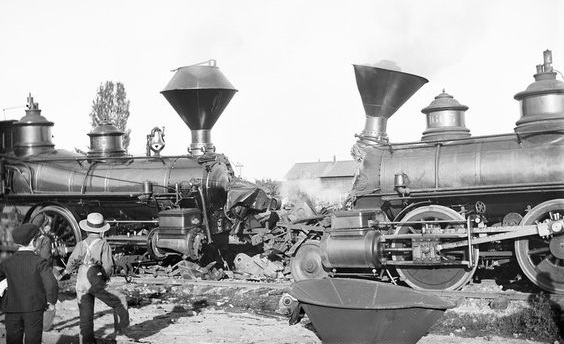
\includegraphics[width=0.8\linewidth]{BZT.jpg}
  \end{center}
}

\part{BZT}\label{part:BZT}
\parttoc

\ifthenelse{ \equal{\DebugMode}{true} }{
% Debug mode ON
  % !TeX spellcheck = cs_CZ
%{\tikzset{external/prefix={tikz/PZT/}}
% \tikzset{external/figure name/.add={ch02_}{}}
%---------------------------------------------------------------------------------------------------
% file ra3ch001.tex
%---------------------------------------------------------------------------------------------------
%======================== Kapitola: Železniční zabezpečovací technika ============================
%\begin{Czech}
\chapter{Obsah zabezpečovací techniky}\label{bzt:chapI}
\minitoc
  Důležitým odvětvím v železniční dopravě je odvětví zabezpečovací techniky. Potřeba zabezpečení 
  železničního provozu vznikala již v prvních začátcích železniční dopravy, ale postupný rozvoj 
  železniční dopravy si vynutil stále větší požadavky na konstrukci nových druhů zařízení a na 
  odbornost pracovníků pro jejich obsluhu.
  
  Tyto příručka je určena jako studijní materiál nezbytný pro implementaci moderních 
  metod návrhu zabezpečovacích systémů v železniční dopravě. 
   
\section{Náplň zabezpečovací techniky}
  Klasická železniční zabezpečovací zařízení jsou definována jako zařízení, která prvořadě 
  kontrolují, zda zamýšlené disposice dopravních zaměstnanců jsou bezpečné a zda jím nařízené 
  výkony se provádějí tak, aby nebyla ohrožena bezpečnost železniční dopravy. Pro přiblížení 
  uvažujme část stanice podle obr. \ref{zzt:fig001} a na této situaci s určitými zjednodušeními 
  tento obsah naznačme.

  \begin{figure}[ht!] %\ref{zzt:fig001}
    \centering
    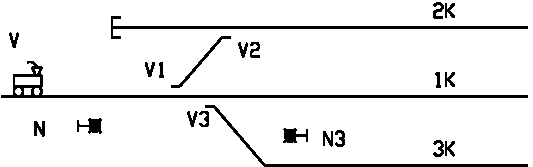
\includegraphics[width=0.8\linewidth]{zzt_fig001.pdf}
    \caption{Stanice
             (\cite[s.~5]{Chudacek2005})}
    \label{zzt:fig001}
  \end{figure}
 
  Před stanicí je umístěno návěstidlo \(N\), které v základní poloze ukazuje návěst \uv{stůj}. Dokud
  návěstidlo ukazuje tuto návěst, nesmí vlak \(V\) do stanice vjet. Má-li vlak vjet bezpečně např. 
  na kolej \(1K\), je třeba splnit určité podmínky. Výměny - pohyblivé části výhybek - \(V1\) a 
  \(V3\) musí být v poloze umožňující řádnou jízdu na kolej \(1K\), tj. jeden jazyk musí
  vždy přiléhat k příslušné opornici, druhý musí být od své opornice náležitě vzdálen. Na koleji 
  \(1K\) (včetně výhybek \(V1\) a \(V3\)) nesmí být žádná vozidla a ani nesmí být povolen příjezd
  jiných vozidel na tuto kolej z opačného směru. Zamýšlenou cestu nesmí ohrožovat z boku pohyby 
  jiných vlaků nebo posunujících dílů, proto výměna \(V2\) musí kolizní jízdu svou polohou 
  znemožňovat a návěstidlo \(N3\) musí kolizní jízdu zakazovat (ochrana odvratnou polohou výměny se 
  nazývá \emph{přímou boční ochranou}, ochrana návěstidlem se zakazující návěstí je \emph{nepřímou 
  boční ochranou}). Když tedy byly všechny prvky zvolené cesty správně nastaveny, přezkoušeny a 
  shledány bez závady, může být návěstidlo \(N\) přestaveno do polohy dovolující jízdu. Po celou 
  dobu, kdy návěstidlo dovoluje jízdu, bude dohlíženo, že všechny k tomu rozhodující podmínky jsou 
  nadále splněny. Vlak \(V\) vjede do stanice a ihned po jeho vjezdu se návěstidlo \(N\) přestaví 
  opět do základní polohy (návěst "stůj"), aby týž povel návěstidla nemohl být využit více vlaky a 
  aby shora uvedený postup bylo třeba pro každý vlak znovu opakovat.

  \begin{figure}[ht!] %\ref{zzt:fig002}
    \centering
    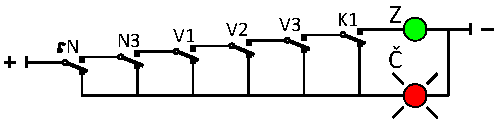
\includegraphics[width=0.8\linewidth]{zzt_fig002.pdf}
    \caption{Vybavení koleje technickým zařízením, které dohlíží na aby vlak vjel do stanice 
             bezpečně
             (\cite[s.~5]{Chudacek2005})}
    \label{zzt:fig002}
  \end{figure}
  
  Úkony, potřebné k tomu, aby vlak vjel do stanice bezpečně, může vykonat určený zaměstnanec. Ten
  se například pochůzkou přesvědčí, že kolej \(1K\) je volná, že výměny jsou řádně postaveny atd. a 
  po ověření všech podmínek přestaví návěstidlo \(N\) do polohy povolující jízdu. Pokud se 
  zaměstnanec nezmýlí, nedojde k nehodě (povšimněme si, že negace této věty nemusí být pravdivá). 
  Bezpečnost jízdy vlaku bude tedy závislá na osobních vlastnostech člověka. Aby tomu tak nebylo, 
  vybavíme koleje technickým zařízením, které bude na jejich volnost dohlížet, výměny jinými
  technickými zařízeními, která budou kontrolovat jejich polohu atd. a jízdní návěst návěstidel
  učiníme nuceně závislou na informacích těchto technických zařízení. Primitivní schéma
  takového zařízení je na obr. \ref{zzt:fig002}. I když pak dopravní zaměstnanec dá návěstním 
  řadičem \(N\) pokyn k rozsvícení jízdní (tj. jízdu povolující) návěsti \(Z\), návěst se rozsvítí 
  jen v případě, že kontakt \(N3\) informuje svým sepnutím, že návěstidlo \(N3\) skutečně ukazuje 
  návěst "stůj", kontakty \(V1\), \(V2\) a \(V3\) informují, že výměny jsou ve správné poloze a 
  kontakt \(K1\) informuje, že první kolej je volná a není na ni postavena jiná cesta. Jízdní 
  návěst \(Z\) se tedy rozsvítí až po splnění všech předem stanovených podmínek pro bezpečný vjezd 
  vlaku. Není-li kterákoliv podmínka splněna, na návěstidle \(N\) zůstává svítit červené světlo Č. 
  
  Přesto takové zařízení \textbf{nelze} považovat za zabezpečovací zařízení. Prvním důvodem je, že 
  nebyly zřízeny \emph{vzájemné závislosti}. Jízdní návěst na návěstidle \(N\) se sice rozsvítí až 
  když jsou splněny všechny podmínky, ale výměny a návěstidla zůstala volná. Nic nebrání, aby se 
  např. poloha výměn změnila dříve, než vlak \(V\) ukončí svou jízdu. Zhasnutí jízdního znaku \(Z\) 
  na návěstidle \(N\) v důsledku ztráty kontroly při přestavení výměny už nemusí být nic platné, 
  protože vlak již mohl návěstidlo minout nebo již není schopen včas zastavit. Nepostačí ale ani 
  zřízení vzájemné závislosti tím, že by rozsvícená jízdní návěst \(Z\) uzavírala výměny a 
  návěstidla v žádoucí poloze (např. prostřednictvím sériově řazeného relé). Vzhledem k nebezpečí
  přerušení sekvence postupných kroků je důležité, aby uzavření výměn a návěstidel bylo provedeno 
  dříve, než se rozsvítí jízdní návěst. Postup stavění jízdní cesty, vyhovující požadavkům 
  zabezpečovací techniky, bude tedy v naznačeném příkladě následující:
  \begin{itemize}\addtolength{\itemsep}{-0.5\baselineskip}
    \item nejprve se přestaví výměny do žádané polohy,
    \item v druhém úkonu (nazývaném závěr jízdní cesty) se při uzavírání výměn a návěstidel 
          přezkouší jejich správná poloha a tedy, že první úkon byl řádně proveden. Pokud první 
          úkon nebyl proveden správně, musí být znemožněn úkon druhý,
    \item obdobně třetí úkon, tj. rozsvícení jízdní návěsti na návěstidle \(N\), je možný jen 
          tehdy, byl-li druhý úkon (a tedy i první úkon) řádně proveden. 
  \end{itemize}
  
  Tím jsme dosáhli požadované \emph{vzájemné závislosti}, jejíž popsaná úroveň je \textbf{prvním
  charakteristickým rysem} zabezpečovacího zařízení. Zařízení z obr. \ref{zzt:fig002} bude podmínce 
  vyhovovat například v případě, že návěstní přepínač \(N\) bude konstrukčně upraven tak, že ho 
  nebude možné přeložit bez provedení \textbf{závěru jízdní cesty}. Důsledkem zavedení závěru 
  jízdní cesty bude potřeba po vlaku jízdní cestu vybavit, tj. závěr zrušit, aby bylo možné s 
  jednotlivými prvky opět volně manipulovat. 

  Ani nyní však ještě nelze v uvedeném příkladě hovořit o zabezpečovacím zařízení. Zařízení musí
  být konstruováno tak, aby \emph{bezpečnost byla zachována i při jakékoliv možné poruše vlastního 
  zařízení}. Tento  požadavek platí jak pro jednotlivé části, tak pro celek a je \textbf{druhým 
  charakteristickým rysem} železniční zabezpečovací techniky. V uvedeném případě to znamená, že 
  zařízení pro kontrolu volnosti koleje nesmí ani při poruše hlásit obsazenou kolej jako volnou, 
  zařízení pro kontrolu polohy výměny nesmí ani při poruše hlásit nesprávně postavenou výměnu jako 
  výměnu správně postavenou, ke zrušení závěru jízdní cesty nesmí ani poruchou dojít dříve než vlak 
  dotčené prvky skutečně mine atd. Právě tak vlastní zapojení pro rozsvícení jízdní návěsti musí 
  být konstruováno tak, aby se jízdní návěst nemohla poruchou zapojení rozsvítit, pokud všechny 
  podmínky pro její svícení nebudou splněny. Jak patrno, vychází se ze základního železničního
  bezpečnostního předpokladu, že zastavení vlaku poskytuje nejvyšší bezpečnost. Tento předpoklad se 
  zásadně liší od principů aplikovaných v letecké dopravě, kosmonautice, nukleární technice, 
  navigaci, řízení procesů, robotice, dolování, systémech zabezpečení proti vloupání či odcizení 
  atd., kde je prozatím obvykle hlavním cílem dosažení maximální spolehlivosti a pohotovosti 
  systému.
  
  Důsledkem druhého charakteristického rysu zabezpečovací techniky, tj. převedení všech poruch
  bezpečnějším směrem je, že téměř každá porucha zabezpečovacího zařízení znamená omezení dopravy. 
  To samozřejmě může vést k narušení plynulosti a vzniku provozních nepravidelností, což jsou jevy, 
  které samy o sobě nebezpečí v dopravě výrazně zvětšují. Ve vážnějších případech je nutné 
  zabezpečovací zařízení do skončení jeho opravy zcela vypnout, aby byl možný alespoň omezený pohyb 
  vlaků. Pak se ovšem provoz, jehož pravidelnost je navíc narušena, děje bez jakékoliv podpory 
  zabezpečovacího zařízení, zatížen, byť i jen na omezenou dobu, možnými lidskými omyly. Odtud tedy 
  plyne třetí charakteristický rys zabezpečovací techniky, což je taková konstrukce zařízení, která 
  má co nejméně poruch, tedy vysokou spolehlivost nebo - obecněji - co nejvyšší pohotovost. 
 
  Úloha zabezpečovací techniky nekončí zajištěním odpovídajícího návěstního znaku na návěstidle.
  Také na lokomotivě je strojvedoucí, jemuž je svěřena péče o bezpečnost vlaku a který tuto 
  bezpečnost může ohrozit svým omylem. Působnost zabezpečovacích zařízení se tedy (prostřednictvím 
  vlakového zabezpečovacího zařízení) prodlužuje až na vozidlo, aby se zajistilo, že vlak také 
  skutečně bude návěsti respektovat. 

  Aplikují-li se všechny výše uvedené zvláštnosti správně při vývoji zabezpečovacího systému, je
  třeba se postarat také o to, aby nedošlo k jejich znehodnocení při projekci, výrobě, montáži a 
  údržbě konkrétních zařízení. Při těchto činnostech je také třeba počítat s lidskými vlastnostmi. 
  Zařízení, sloužící primárně pro eliminaci chyb dopravních zaměstnanců konstruují, vyrábějí, 
  montují a udržují opět lidé. Naštěstí tyto práce, na rozdíl od výkonu dopravní služby, probíhají 
  (nebo by rozhodně měly probíhat) v lepších podmínkách a bez časové tísně. Za příznivých podmínek 
  se nedokonalosti člověka tolik neuplatňují a práci každého pracovníka lze kontrolovat jinými s 
  případnou pomocí dalších technických zařízení. Přesto však z toho pro projekci, výrobu, montáž a 
  údržbu zabezpečovacích zařízení vyplývají jisté zvláštnosti. 
  
  Vedle úloh z oblasti bezpečnosti plní moderní zabezpečovací technika i úkoly další. Především jde
  o hlubší zásahy do vlastního provozu prostředky automatizace. Ta pak, při správném provedení, 
  vede k zlepšenému využití technických prostředků železnic (např. zvýšení propustné výkonnosti 
  tratí), k zhospodárnění provozu, k úspoře jiných, podstatně vyšších investičních nákladů (např. 
  budování další koleje). Protože však zabezpečovací zařízení je zařízením v zásadě restriktivním, 
  nelze u něj bezhlavě prosazovat zvyšování výkonnosti vždy a ve všech směrech. Později také 
  uvidíme, že zabezpečovací technika se podílí na zvyšování bezpečnosti i v jiných oblastech: 
  kolejové obvody alespoň částečně dohlíží na stav jízdní dráhy (celistvost kolejnic), přestavná 
  zařízení výměn dohlíží na stav výhybek, vlakové zabezpečovače mohou do určité míry dohlížet na 
  stav brzdové soustavy vlaku (sledováním skutečně dosaženého odrychlení při brzdění), přejezdová 
  zabezpečovací zařízení se podílejí na eliminaci cizích vlivů na dopravu atd.
  
  Souhrnně lze konstatovat, že prvořadým účelem zabezpečovacích zařízení na železnici je
  předcházet kolizím a vykolejení vlaků z důvodu chybného řízení dopravy. K tomu účelu je u 
  zařízení třeba sledovat následující oblasti:
  \begin{itemize}\addtolength{\itemsep}{-0.5\baselineskip}
    \item funkční bezpečnost (korektnost systému), tj. řádné plnění všech požadovaných funkcí v 
          bezporuchovém stavu a při očekávaných vlivech pracovního prostředí,
    \item technickou bezpečnost (bezpečnou konstrukci), tj. splnění požadavku, aby nedošlo k 
          přímému ohrožení bezpečnosti dopravy ani při poruchách samotného zabezpečovacího zařízení,
    \item bezpečnou aplikaci, tj. vytvoření takových logických funkcí a vzájemných závislostí, aby 
          pro konkrétní situaci navržené zařízení ve všech provozních stavech mohlo řádně plnit 
          svou funkci (na jeho výstupech budou jízdu povolující informace pouze v takovém rozsahu, 
          který odpovídá stavu informací vstupních) a zajištění, aby tyto vlastnosti zařízení mělo 
          i po výrobě a montáži,
    \item bezpečný provoz a údržbu, tj. zajištění, že předchozí úrovně zůstanou v zařízení 
          zachovány po celou dobu životnosti,
    \item vysokou spolehlivost, tj. omezení případů, kdy nepřímo, vyřazením zabezpečovacího 
          zařízení a přechodem na manuální řízení, by mohlo dojít k ohrožení bezpečnosti dopravy.
  \end{itemize}
  Žádnou ze zmíněných oblastí nelze preferovat, protože žádná nemůže nahradit druhou a             
  nedostatky v kterékoliv z nich znehodnocují výsledky ostatních.
  
  Přímým obsahem železniční zabezpečovací techniky není zajištění zdraví a bezpečnosti
  zaměstnanců (i když provozovaná zařízení samozřejmě musí splňovat i požadavky např. ve směru 
  ochrany před nebezpečným dotykovým napětím, ergonomicky správně navrženého obsluhovací pracoviště 
  atd.), zabránit nehodám ze zlého úmyslu, násilnou obsluhou, úmyslným poškozením nebo zneužitím 
  zařízení. V poslední době se však jeví jako nezbytné dokonaleji zajišťovat zabezpečovací zařízení 
  proti vandalům a lapkům všeho druhu a neoprávněným zásahům do zařízení v případě, že používají 
  jiných než speciálně drážních zařízení (viz dále např. ochrana dat v otevřených sítích).  

\section{Třídění}
  K železničním zabezpečovacím zařízením se obvykle řadí i zabezpečovací zařízení používaná na
  podzemních drahách (metro, doly), na pouličních drahách (tramvaje - zejména městské rychlodráhy) 
  a na vlečkách, protože využívají obdobných principů, často i obdobná nebo jen poněkud upravená 
  zařízení. Při třídění zařízení lze použít řadu třídících hledisek; téměř vždy se však vyskytnou 
  zařízení přechodová (smíšená) nebo podle užitého třídění obtížně definovatelná. Přesto je dále 
  několik třídění uvedeno, protože poskytují obrázek o pestrosti a mnohotvárnosti pojednávaného 
  zařízení. 
  
  Nejpřirozenějším a klasickým tříděním zabezpečovacích zařízení je třídění podle účelu zařízení.
  Podle tohoto hlediska lze zabezpečovací zařízení dělit na zařízení: 
  \begin{itemize}\addtolength{\itemsep}{-0.5\baselineskip}
    \item staniční,
    \item traťové,
    \item vlakové,
    \item přejezdové, 
    \item spádovištní. 
  \end{itemize}
  Účel je patrný již z názvu. Staniční zabezpečovací zařízení zajišťuje bezpečný pohyb vlaků ve 
  stanici, traťové zařízení zabezpečuje jízdu vlaku na trati mezi stanicemi, vlakové zařízení 
  zabraňuje vlaku pohybovat se nad rámec, který povoluje zařízení staniční a traťové (s případným 
  zahrnutím i dalších omezení), přejezdové zařízení přispívá k zajištění bezpečnosti na úrovňovém 
  křížení silnice a železnice informováním uživatelů silnice, že se k přejezdu blíží vlak s 
  předností v jízdě. Nad všemi těmito zařízeními pak může být budováno zařízení pro dálkové 
  ovládání většího úseku tratě z jednoho místa. 
  
  Podle místa ovládání zařízení mluvíme o zařízení s obsluhou :
    \begin{itemize}\addtolength{\itemsep}{-0.5\baselineskip}
    \item místní,
    \item ústřední (centralizovanou v oblasti jedné stanice),
    \item dálkovou (mimo vlastní stanici).
  \end{itemize}

  Další třídění je odvozeno od způsobu ovládání periferií (výměn, návěstidel atd.) a tak vlastně
  zahrnuje celou historii železniční zabezpečovací techniky. Rozeznáváme zařízení:
  \begin{itemize}\addtolength{\itemsep}{-0.5\baselineskip}
    \item mechanická (využívající výhradně lidské síly),
    \item elektrická,
    \item pneumatická,
    \item hydraulická. 
  \end{itemize}

  Obdobně, v následujícím třídění je rozhodující způsob, jímž se v zařízení potřebné závislosti
  realizují. Zde rozeznáváme zařízení se závislostmi:
  \begin{itemize}\addtolength{\itemsep}{-0.5\baselineskip}
    \item mechanickými,
    \item mechanickými i elektrickými (tzv. elektromechanická a elektrodynamická zařízení),
    \item elektrickými, která lze dále dělit podle rozhodujících stavebních prvků, jimiž jsou 
         závislosti realizovány, na zařízení:
       \begin{itemize}
       \item reléová,
       \item hybridní (rozhodující část bezpečné logiky je realizována reléově, zbytek 
             elektronicky),
       \item elektronická (mikroprocesorová). 
       \end{itemize}
  \end{itemize}

  U traťových zabezpečovacích zařízení je kladen důraz na rozsah spolupůsobení vlaku. Zařízení se
  pak dělí na:
  \begin{itemize}\addtolength{\itemsep}{-0.5\baselineskip}
    \item poloautomatická (poloautobloky),
    \item automatická (autobloky).
  \end{itemize}
  Podle rozmístění traťových zařízení podél trati lze automatická zařízení dále dělit na:
  \begin{itemize}\addtolength{\itemsep}{-0.5\baselineskip}
    \item decentralizovaná (funkční bloky jsou umístěny v každém návěstním bodě),
    \item částečně centralizovaná (funkční bloky jsou umístěny pouze ve vybraných bodech na trati),
    \item centralizovaná (zařízení je koncentrováno do stanic).
  \end{itemize}
  Vlaková zabezpečovací zařízení se dělí podle způsobu přenosu informací mezi tratí a hnacím
  vozidlem na zařízení:
  \begin{itemize}\addtolength{\itemsep}{-0.5\baselineskip}
    \item bodová,
    \item semiliniová,
    \item liniová. 
  \end{itemize}

  Podle způsobu kontroly souladu jízdy vlaku s přenášenými informacemi se vlaková zařízení dále 
  dělí na zařízení s kontrolou:
  \begin{itemize}\addtolength{\itemsep}{-0.5\baselineskip}
    \item bdělosti strojvedoucího,
    \item rychlosti vlaku.
  \end{itemize}
  
  Zařízení přejezdová se dělí podle způsobu výstrahy na přejezdová zařízení:
  \begin{itemize}\addtolength{\itemsep}{-0.5\baselineskip}
    \item mechanická,
    \item světelná bez závor,
    \item světelná se závorami.
  \end{itemize}
  
  U moderních systémů dělení zabezpečovacích zařízení na zařízení staniční, traťová, vlaková a
  přejezdová ztrácí smysl, protože systémy jsou komplexní, se společným jádrem řídícím jednotlivé 
  periférie a tyto celky pak tvoří nanejvýš podsystémy. Na obr. 3-1 je základní blokové schéma 
  takového systému. 
  \begin{figure}[ht!] %\ref{zzt:fig003}
    \centering
    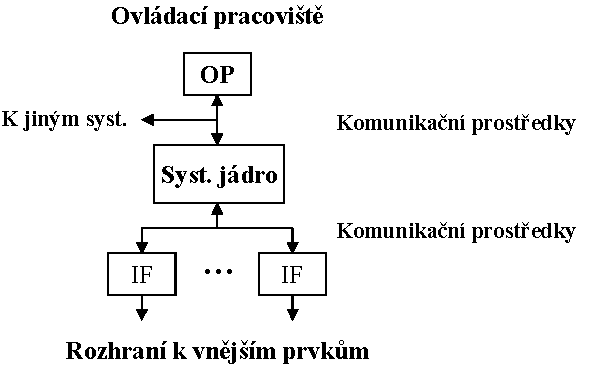
\includegraphics[width=0.8\linewidth]{zzt_fig003.pdf}
    \caption{Stanice
             (\cite[s.~11]{Chudacek2005})}
    \label{zzt:fig003}
  \end{figure}


  \section{Klasifikace poruch}
    \textbf{Chyba} je rozdíl mezi správnou a skutečnou hodnotou nějaké veličiny. V zařízení se 
    chyby mohou obecně objevit jako \emph{důsledek (projev) poruchy některé jeho součásti, 
    působením nějakého cizího vlivu} nebo \emph{selháním lidského činitele}. Za poruchy hardware se 
    považují všechna vybočení z předpokládaných vlastností stavebního prvku (součástky, dílu) 
    zařízení. Předpokládanými vlastnostmi prvků přitom jsou vlastnosti odpovídající příslušným 
    technickým podmínkám popisujícím jeho vlastnosti. Jako omyl lze označit každou lidskou činnost, 
    která může vést k nezamýšlenému chování zařízení. V širším slova smyslu se jako 
    \textbf{porucha} označují souhrnně všechny příčiny vedoucí k chybě, tj. poruch součásti, 
    cizí vliv i omyl.

%~~~~~~~~~~~~~~~~~~~~~~~~~~~~~~~~~~~~~~~~~~~~~~~~~~~~~~~~~~~~~~~~~~~~~~~~~~~~~~~~~~~~~~~~~~~~~~~~~~
\printbibliography[title={Seznam literatury}, heading=subbibliography]
\addcontentsline{toc}{section}{Seznam literatury}

\chapter{Bezpečnost a spolehlivost zabezpečovacích systémů}
 \section{Spolehlivost}
 \section{Bezpečnost}
    V různých publikacích je možné najít různé definice bezpečnosti. Například norma 
    EN~61508\footnote{Funkční bezpečnost elektrických/elektronických/programovatelných 
    elektronických systémů souvisejících s bezpečností (Functional safety of electrical/ 
    electronic/programmable electronic systems), obecná norma funkční bezpečnosti, která se opírá o 
    dvě základní koncepce - životní cyklus bezpečnosti a úroveň integrity bezpečnosti 
    (\texttt{SIL})} 
    definuje bezpečnost jako nepřítomnost netolerovaného rizika. Z této definice je zřejmé, že 
    bezpečnost je úzce spjatá s rizikem, a je nutné bezpečnost třeba chápat relativně. Když se 
    řekne, že řídicí systém je bezpečný, neznamená to jeho absolutní bezpečnost (ta je prakticky 
    nedosažitelná vzhledem na existenci objektivních faktorů, jako je například úroveň poznání, 
    technologická úroveň a limitované finanční prostředky), ale taková úroveň bezpečnosti, 
    která zodpovídá definovaným bezpečnostním požadavkům na tento řídicí systém. 

    Relativnost v pojímání bezpečnosti znamená posun od kvalitativního ke kvantitativnímu chápaní bezpečnosti.

    Kvalitativně je bezpečnost chápána jako schopnost řídicího systému zajistit omezení důsledků 
    poruch řídicích systému v daných podmínkách a v daném časovém intervalu. Matematicky je možné 
    kvalitativní bezpečnost řídicího systému vyjádřit jako 
    \begin{equation}
      E_H = 0,
    \end{equation}
    kde \(E_H\) je množina nebezpečných stavů, které jsou důsledkem výskytu pravděpodobných poruch 
    řídicího systému. Pravděpodobná porucha je taková porucha z množiny všech poruch, jejichž 
    výskyt během provozu řídicího systému je nutné předpokládat (vzhledem na požadovanou úroveň 
    bezpečnosti řídicího systému).
	
    Kvantitativně je bezpečnost řídicího systému chápána jako pravděpodobnost nepřítomnosti
    jakéhokoliv nebezpečného stavu v řídicím systému v daných podmínkách a v daném časovém
    intervalu. Je zřejmé, že i když pravděpodobnost nebezpečného stavu řídicího je malá, neznamená
    to, že se nebezpečný stav nemůže vyskytnou v nejbližším časovém intervalu, Matematicky je možné
    kvantitativní bezpečnost vyjádřit tak, že
    \begin{equation}
      P_{HT}(t)\geq P_{HT}(t)>0,
    \end{equation}
    kde \(P_{HT}(t)\) je pravděpodobnost tolerovaného nebezpeční řídicího systému a \(P_{HR}(t)\)
    je reálná pravděpodobnost nebezpeč\-ného stavu řídicího systému.
	 
    Na kvantitativním hodnocení bezpečnosti řídicího systému je v podstatě možné uplatnit stejné 
    teoretické postupy, jako při hodnocení spolehlivosti technických systémů. Zásadní rozdíl je v 
    tom, že při hodnocení spolehlivosti standardních řídicích systémů se obvykle rozlišují dva 
    stavy - bezporuchový stav a poruchový stav, a k těmto dvěma stavům se vztahují také 
    kvantitativní ukazatele spolehlivosti. Při hodnocení bezpečnosti řídicích systémů musíme 
    uvažovat s dvěma druhy poruchových stavů - bezpečným a nebezpečným poruchovým stavem. 
    Bezpečnost řídicího systému se potom vyjadřuje pomocí ukazatelů bezpečnosti (například 
    pravděpodobnost výskytu nebezpečné poruchy, intenzita nebezpečných poruch, ...).

    Při kvantitativním hodnocení důsledků poruch na bezpečnost řídicího systému se obvykle k 
    hodnoceným řídicím systémům přistupuje jako k neobnovovaným objektům, protože z pohledu 
    bezpečnosti jsou důležité dva stavy (bezpečný, nebezpečný) a analýza končí výskytem nebezpečné 
    poruchy (může jít o jednu poruchu, nebo o kombinaci více poruch, které nejsou individuálně 
    nebezpečné). To znamená, že od uvedení řídicího systému do provozu, až po výskyt nebezpečné 
    poruchy, se může řídicí systém střídavě nacházet ve funkčním, nebo nefunkčním stavu (nefunkční 
    ještě neznamená nebezpečný). Z tohoto důvodu ukazatele bezpečnosti jsou podobné ukazatelům 
    bezporuchovosti neobnovovaných objektů. 
  
    \subsection{Základní legislativa}
      \begin{itemize}
        \item \textbf{EN 61508} - \emph{základní všeobecná norma pro SRCS}; pojednává o funkční
              bezpečnosti elektrických/elektronických/programovatelných elektronických systémů
              souvisejících s bezpečností (Functional safety of electrical/electronic/programmable
              electronic systems), obecná norma funkční bezpečnosti, která se opírá o dvě základní
              koncepce - životní cyklus bezpečnosti a úroveň integrity bezpečnosti (\texttt{SIL})
              \begin{itemize}
                \item EN 61508-1: Všeobecné požadavky
                \item EN 61508-2: Požadavky na elektrické / elektronické / programovatelné
                                  elektronické systémy související s bezpečností
                \item EN 61508-3: Požadavky na SW
                \item EN 61508-4: Definice a zkratky
                \item EN 61508-5: Příklady metod určování úrovně integrity bezpečnosti
                \item EN 61508-6: Metodické pokyny na používání EN 61508-2, STN EN 61508-3
                \item EN 61508-7: Přehled technik a opatření
              \end{itemize}
        \item \textbf{EN 50126}: Railway applications – The specification and demonstration of
              reliability, availability, maintainability and safety (RAMS)
              \begin{itemize}
                \item Part 1: Basic requirements and generic process. 1999
                \item Part 2: Guide to the application of EN 50126-1 for safety. 2007
                \item Part 3: Guide to the application of EN 50126-1 for rolling stock RAMS. 2008  
              \end{itemize}
              Zabývá se specifikací parametrů RAMS (spolehlivost, pohotovost, udržovatelnost,
              a bezpečnost) obecně pro všechny železniční systémy, reaguje na skutečnost, že
              naléhavost požadavků na bezpečnost funkce jednotlivých železničních systémů je různá
              a lze je tedy splňovat s různou pravděpodobností jejich selhání. Také zavádí pojem
              \emph{integrita bezpečnosti (safety integrity - celistvost, úplnost, neporušenost
              bezpečnosti)}, který definuje jako pravděpodobnost, s níž systém uspokojivě splní
              požadované bezpečnostní funkce, za všech stanovených podmínek a ve stanoveném časovém
              období. Jde o to, do jaké míry může být pro bezpečnost relevantní funkce narušena
              např. poruchami vlastního zařízení, omyly obsluhy, vnějším rušením atd.
        \item \textbf{EN 50128}: Railway applications – Communication, signalling and processing
              systems – Software for railway control and protection systems. 2003          
        \item \textbf{EN 50129}: Railway applications – Communication, signalling and processing
              systems – Safety-related electronic systems for signalling. 2011
              Modifikovaně byl pojem integrita bezpečnosti přenesen i do této normy pro železniční
              zabezpečovací systémy. I klasická zabezpečovací technika bez velkého zdůrazňování
              respektovala, že nejsou na všechna zařízení kladeny stejně důrazné bezpečnostní
              požadavky (kategorie zařízení, vedlejší tratě/hlavní tratě, zařízení pro ČD/zařízení
              pro vlečky, staniční zařízení/spádoviště atd.). Uvidíme dále, že pojmu integrita
              bezpečnosti je pro zabezpečovací zařízení dominantně obsažena oblast, kterou běžně v
              této technice označujeme(a také normá EN 50129 ji tak označuje ve své základní části)
              termínem technická bezpečnost. Úvahy okolo integrity bezpečnosti zde sledujeme
              odděleně od úvah o technické bezpečnosti (přes jejich podobnost) pro jejich výhodnost
              zejména v úvodních fázích projektu nového systému (zařízení, výrobku, atd.)
        \item \textbf{EN 50159: Railway applications – Communication, signalling and processing
              systems - Safety-related communication in transmission systems. 2010}            
      \end{itemize}
    
      Vyjmenované normy se poněkud liší v definici termínu \emph{bezpečnost}:  
      \begin{itemize}
        \item Bezpečnost (Safety) – nepřítomnost nepřijatelných úrovní rizika poškození (EN50129)
        \item Bezpečnost (Safety) – nepřítomnost nepřijatelného rizika. (EN61508)
        \item Bezpečnost při poruše (Fail Safe) – vlastnost konstrukce objektu zabraňující,
              aby jeho poruchy způsobili nebezpečné poruchové stavy. (IEC 50 (191))
        \item Kvalitativní bezpečnost – schopnost systému zajistit omezení důsledku poruch
              systému v daných podmínkách a v daném časovém intervale.
        \item Kvantitativní bezpečnost – pravděpodobnost nepřítomnosti jakéhokoliv
              nebezpečného stavu v systéme v daných podmínkách a v daném časovém intervale.
      \end{itemize}

    \subsection{Ukazatel bezpečnosti}
      \fbox{Pravděpodobnost bezpečného provozu} je pravděpodobnost, že objekt může bezpečně plnit 
      požadovanou funkci v daných podmínkách v časovém intervalu \(t_1,\, t_2\).
      \begin{equation}
        R_S(t_1,\, t_2) = 1- F_H(t_1,\, t_2),
      \end{equation}
      kde \(F_H(t_1,\, t_2)\) je distribuční funkce, která naopak vyjadřuje pravděpodobnost, že
      objekt nemůže bezpečně plnit požadovanou funkci k daným podmínkám v časovém intervalu
      \(t_1,\, t_2\).
      \begin{equation}
        F_H(t_1,\, t_2) = \int_{t_1}^{t_2}f_H(t)\cdot\dd{t},
      \end{equation}
      kde \(f_H(t)\) je hustota pravděpodobnosti nebezpečné poruchy objektu. 

      \fbox{Intenzita nebezpečných poruch} \(\lambda_H(t)\) definujme jako limitu poměru podmíněné
      pravděpodobnosti, že časový okamžik vzniku nebezpečné poruchy objektu \(T\) padne do daného
      časového intervalu \(t,\, t+\Delta t\), přičemž délka časového intervalu \(\Delta
      t\rightarrow0\)
      \begin{equation}\label{DZT:eq_def_lambdaH}
        \lambda_H=\frac{f_H(t)}{R_S(t)}.
      \end{equation}

      Protože nebezpečné poruchy jsou méně časté, zkoušky na určení požadovaných ukazatelů
      bezpečnosti by bylo třeba provádět dlouhodobě, což je prakticky nemožné. 
    
  \section{Integrita bezpečnosti}
    Všeobecně je možné konstatovat, že SRCS realizuje řídící i ochranné funkce (obr.
    \ref{DZT:fig_DZT_SRCS_fce}). Jelikož selhání řídicí funkce může způsobit ohrožení bezpečnosti,
    je třeba i tyto funkce považovat za bezpečnostní.
    \begin{figure}[hb!]
      \centering
      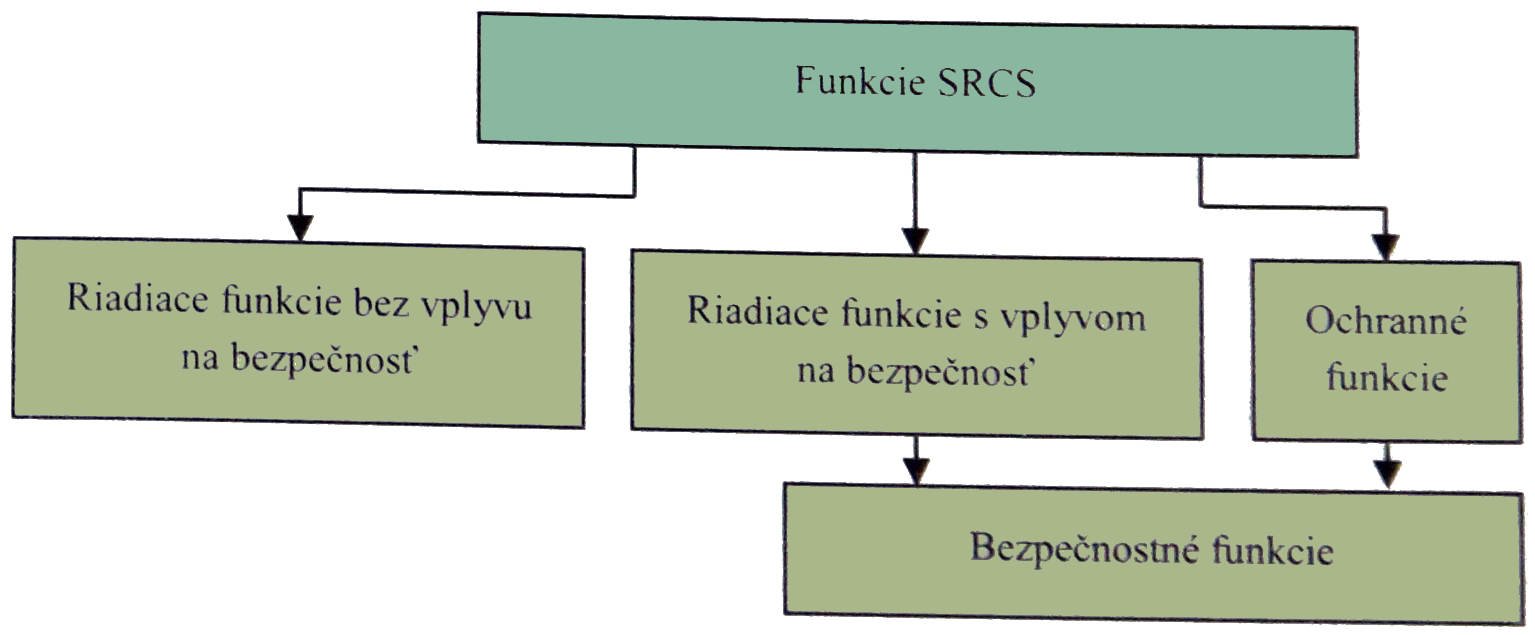
\includegraphics[width=1\linewidth]{DZT_SRCS_fce.jpg}
      \caption{Vztah mezi bezpečnostními funkcemi a moduly SRCS}
      \label{DZT:fig_DZT_SRCS_fce}
    \end{figure}    
    Bezpečnostní funkce jsou definované na základě analýzy rizik jako technická opatření na snížení
    rizika spojeného s konkrétními nebezpečí na tolerovatelnou úroveň. Účinnost bezpečnostní funkce
    se určuje pomocí úrovně integrity bezpečnosti \emph{(\texttt{SIL} - safety integrity level)}. 
    
    Norma \emph{EN 61508} definuje integritu bezpečnosti jako pravděpodobnost, že SRCS bude plnit 
    požadované bezpečné funkce za všech stanovených podmínek v rámci stanoveného operačního 
    prostředí a během stanoveného časového období. Všeobecně lze konstatovat, že čím je integrita
    bezpečnosti SRCS větší, tím je menší pravděpodobnost selhání bezpečností funkce realizovaných
    SRCS.  
    
    Integrita bezpečnosti se skládá ze dvou částí a to:
    \begin{itemize}
      \item \emph{integrity bezpečnosti proti systematickým poruchám}: jde o nekvantifikovatelnou
            část integrity bezpečnosti, která souvisí s nebezpečnými systematickými poruchami 
            hardware a software; integrity bezpečnosti proti systematickým poruchám se dosahuje
            především opatřeními na předcházení chybám a poruchám; vzhledem k tomu, že jde o 
            nekvantifikovatelnou část integrity bezpečnosti, je vhodnější chápat integritu 
            bezpečnosti jako vlastnost a né jako pravděpodobnost; hodnocení integrity bezpečnosti
            proti systematickým chybám a poruchám se realizuje kontrolou dodržování opatření
            předcházejících chybám a poruchám, mezi které patří také důsledné testování korektní
            realizace bezpečnostních funkcí; 
      \item \emph{integrity bezpečnosti proti náhodným poruchám}: jde o kvantifikovatelnou část
            integrity bezpečnosti, která se týká náhodných poruch hardware vyplývajících z konečné
            bezporuchovosti použitých součástek; hodnocení integrity bezpečnosti proti náhodným
            poruchám se realizuje prostřednictvím pravděpodobnostních výpočtů.
    \end{itemize}
    
    Aby se dosáhla požadovaná integrita bezpečnosti, musí být splněné požadavky na integritu proti 
    systematickým poruchám i náhodným poruchám. 
    
    \subsection{Úroveň integrity bezpečnosti}
      Úroveň integrity bezpečnosti (\emph{Safety Integrity Levels - \texttt{SIL}}) se dělí podle EN 
      50129
      do čtyř kategorií - úroveň 4 (\texttt{SIL} 4) je nejvyšší, úroveň 1 (\texttt{SIL} 1) je 
      nejnižší.  Pokud se
      objevuje úroveň \texttt{SIL} 0, značí to, že se jedná o systém na které nejsou kladeny žádné
      bezpečnostní požadavky (ve smyslu zabezpečovací techniky)
      
      Proto, aby SRCS mohl být zařazen do odpovídající úrovně bezpečnosti \texttt{SIL}, musí 
      vyhovovat
      těmto faktorům:
      \begin{itemize}
        \item naplnění podmínek řízení kvality, 
        \item naplnění podmínek řízené bezpečnosti,
        \item splnění požadavků na technickou bezpečnost, 
        \item dosažení kvantitativního cíle
      \end{itemize}
      
      Jak patrno, splnění kvantitativního ukazatele samo o sobě neznamená, že bylo dosaženo
      odpovídající úrovně bezpečnosti. To platí ovšem i naopak - splnění tří předchozích podmínek
      (řízení kvality, řízení bezpečnosti a technické bezpečnosti) nezaručuje, že bylo dosaženo
      kvantitativních cílů a nelze tedy tvrdit, že zařízení lze zařadit do odpovídající skupiny
      \texttt{SIL} (\ref{DZT:fig_EN50129_SIL_techniques}).
      
      \begin{figure}[ht!]% Relationship between \texttt{SIL}s and techniques
        \centering
        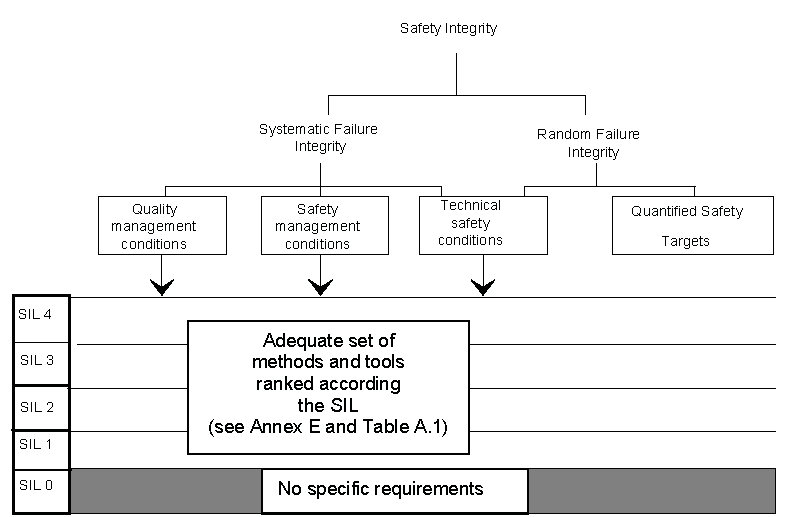
\includegraphics[width=0.95\linewidth]{EN50129_SIL_techniques.pdf}
        \caption{Vztah mezi \texttt{SIL} úrovní a technikami jejich dosažení}
        \label{DZT:fig_EN50129_SIL_techniques}
      \end{figure}
      
      Žádná z norem \texttt{CENELEC} nepředepisuje, které zařízení musí být jaké úrovně. Toto 
      určení je 
      ponecháno na provozovateli, resp. regulátorovi, vyplyne také z provedených analýz rizik 
      a hazardů.
      
      Následující tabulka shrnuje definované úrovně integrity bezpečnosti a zároveň dává do
      souvislosti s tolerovatelnými četnostmi hazardů. \texttt{SIL} jsou tedy prostředkem přiřazení
      kvalitativních přístupů (pro vyloučení systematických poruch) ke kvantitativnímu přístupu
      (pro řízení náhodných poruch), neboť systematické poruchy nelze kvantifikovat.
      \begin{table}[h]
        \centering
        \begin{tabular}{|c|c|}
          \hline
           Úroveň integrity &  Tolerovatelná četnost hazardu            \\
             bezpečnosti \texttt{SIL} &  THR [za hodinu a funkci]       \\ \hline\hline 
              4        & \(10^{-9}\leq THR < 10^{-8}\)                  \\ \hline
              3        & \(10^{-8}\leq THR < 10^{-7}\)                  \\ \hline
              2        & \(10^{-7}\leq THR < 10^{-6}\)                  \\ \hline
              1        & \(10^{-6}\leq THR < 10^{-5}\)                  \\ \hline
        \end{tabular}
        \caption{\texttt{SIL} tabulka: Funkce, jejichž kvantitativní požadavky by převyšovaly 
                 hranici \(10^{-9}\), která se zdánlivě nelogicky objevuje u \texttt{SIL4}, vyžaduje
                 podle normy \texttt{EN~50129} zvláštní technická nebo provozní opatření pro 
                 dosažení tak mimořádného cíle.}
      \end{table}
       
      \begin{enumerate}
        \item Z normy jasně vyplývá rozdělení na dvě skupiny \texttt{SIL 1,2} vs. \texttt{SIL 3,4}, 
              u nichž je výrazný rozdíl v požadavcích, které je potřeba splnit, aby SRCS mohl 
              patřit do dané skupiny. To je velmi dobře patrné z tabulek v příloze \texttt{E} normy 
              \texttt{EN 50129}, která se zabývá technikami a opatřeními pro řízení náhodných a 
              systematických poruch. 
        \item Druhým důležitým faktem je poněkud odlišná definice chápání úrovní \texttt{SIL} v 
              EN~61508. \emph{Funkční bezpečnost elektrických, elektronických, programovatelných
              elektronických systémů souvisejících s bezpečností}. Tato norma je obecnou normou pro
              průmyslové elektronické systémy, z níž vycházejí normy EN~50126, EN 50~129 atd.
              jakožto specifické normy pro železniční aplikace. Důležitou odlišností ve specifikaci
              \texttt{SIL}, viz tab. 2 a 3 v první části této normy (EN~61508-1). Nicméně tabulka 3 
              pro
              režim provozu s vysokým, resp. nepřetržitým vyžádáním odpovídá tabulce v normě
              EN~50129. Avšak i pro tyto systémy se zde jeví určitá odlišnost v požadavcích na
              zajištění dané \texttt{SIL}. Norma EN~61508 je zaměřena pouze na \emph{funkční 
              bezpečnost},
              není zde zahrnutý požadavek na bezpečnou reakci na ojedinělé náhodné poruchy. S
              poruchami se samozřejmě pracuje, mají být provedena opatření k jejich maximálnímu
              potlačení - četnosti i následku, nicméně může stačit, když systém je schopen poruchy
              detekovat a dát o nich vědět (např. obsluze). Závěrem nutno dodat, že je potřeba
              určité obezřetnosti k tvrzení, že systém splňuje daný \texttt{SIL}. Tento údaj musí 
              být
              doplněn specifikací, která norma byla při klasifikaci použita.
      \end{enumerate}
      
%\end{Czech}

%} %tikzset
%~~~~~~~~~~~~~~~~~~~~~~~~~~~~~~~~~~~~~~~~~~~~~~~~~~~~~~~~~~~~~~~~~~~~~~~~~~~~~~~~~~~~~~~~~~~~~~~~~~
\printbibliography[title={Seznam literatury}, heading=subbibliography]
\addcontentsline{toc}{section}{Seznam literatury}
}
{
 % DEBUG was off
%========== Kapitola 001: Bezpečnost a spolehlivost zabezpečovacích systémů =======================
  % !TeX spellcheck = cs_CZ
%{\tikzset{external/prefix={tikz/PZT/}}
% \tikzset{external/figure name/.add={ch02_}{}}
%---------------------------------------------------------------------------------------------------
% file ra3ch001.tex
%---------------------------------------------------------------------------------------------------
%======================== Kapitola: Železniční zabezpečovací technika ============================
%\begin{Czech}
\chapter{Obsah zabezpečovací techniky}\label{bzt:chapI}
\minitoc
  Důležitým odvětvím v železniční dopravě je odvětví zabezpečovací techniky. Potřeba zabezpečení 
  železničního provozu vznikala již v prvních začátcích železniční dopravy, ale postupný rozvoj 
  železniční dopravy si vynutil stále větší požadavky na konstrukci nových druhů zařízení a na 
  odbornost pracovníků pro jejich obsluhu.
  
  Tyto příručka je určena jako studijní materiál nezbytný pro implementaci moderních 
  metod návrhu zabezpečovacích systémů v železniční dopravě. 
   
\section{Náplň zabezpečovací techniky}
  Klasická železniční zabezpečovací zařízení jsou definována jako zařízení, která prvořadě 
  kontrolují, zda zamýšlené disposice dopravních zaměstnanců jsou bezpečné a zda jím nařízené 
  výkony se provádějí tak, aby nebyla ohrožena bezpečnost železniční dopravy. Pro přiblížení 
  uvažujme část stanice podle obr. \ref{zzt:fig001} a na této situaci s určitými zjednodušeními 
  tento obsah naznačme.

  \begin{figure}[ht!] %\ref{zzt:fig001}
    \centering
    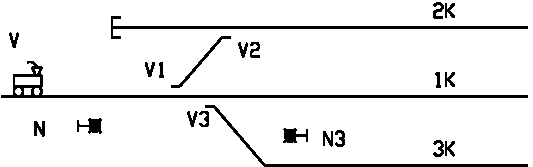
\includegraphics[width=0.8\linewidth]{zzt_fig001.pdf}
    \caption{Stanice
             (\cite[s.~5]{Chudacek2005})}
    \label{zzt:fig001}
  \end{figure}
 
  Před stanicí je umístěno návěstidlo \(N\), které v základní poloze ukazuje návěst \uv{stůj}. Dokud
  návěstidlo ukazuje tuto návěst, nesmí vlak \(V\) do stanice vjet. Má-li vlak vjet bezpečně např. 
  na kolej \(1K\), je třeba splnit určité podmínky. Výměny - pohyblivé části výhybek - \(V1\) a 
  \(V3\) musí být v poloze umožňující řádnou jízdu na kolej \(1K\), tj. jeden jazyk musí
  vždy přiléhat k příslušné opornici, druhý musí být od své opornice náležitě vzdálen. Na koleji 
  \(1K\) (včetně výhybek \(V1\) a \(V3\)) nesmí být žádná vozidla a ani nesmí být povolen příjezd
  jiných vozidel na tuto kolej z opačného směru. Zamýšlenou cestu nesmí ohrožovat z boku pohyby 
  jiných vlaků nebo posunujících dílů, proto výměna \(V2\) musí kolizní jízdu svou polohou 
  znemožňovat a návěstidlo \(N3\) musí kolizní jízdu zakazovat (ochrana odvratnou polohou výměny se 
  nazývá \emph{přímou boční ochranou}, ochrana návěstidlem se zakazující návěstí je \emph{nepřímou 
  boční ochranou}). Když tedy byly všechny prvky zvolené cesty správně nastaveny, přezkoušeny a 
  shledány bez závady, může být návěstidlo \(N\) přestaveno do polohy dovolující jízdu. Po celou 
  dobu, kdy návěstidlo dovoluje jízdu, bude dohlíženo, že všechny k tomu rozhodující podmínky jsou 
  nadále splněny. Vlak \(V\) vjede do stanice a ihned po jeho vjezdu se návěstidlo \(N\) přestaví 
  opět do základní polohy (návěst "stůj"), aby týž povel návěstidla nemohl být využit více vlaky a 
  aby shora uvedený postup bylo třeba pro každý vlak znovu opakovat.

  \begin{figure}[ht!] %\ref{zzt:fig002}
    \centering
    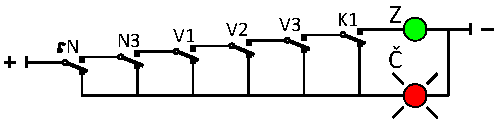
\includegraphics[width=0.8\linewidth]{zzt_fig002.pdf}
    \caption{Vybavení koleje technickým zařízením, které dohlíží na aby vlak vjel do stanice 
             bezpečně
             (\cite[s.~5]{Chudacek2005})}
    \label{zzt:fig002}
  \end{figure}
  
  Úkony, potřebné k tomu, aby vlak vjel do stanice bezpečně, může vykonat určený zaměstnanec. Ten
  se například pochůzkou přesvědčí, že kolej \(1K\) je volná, že výměny jsou řádně postaveny atd. a 
  po ověření všech podmínek přestaví návěstidlo \(N\) do polohy povolující jízdu. Pokud se 
  zaměstnanec nezmýlí, nedojde k nehodě (povšimněme si, že negace této věty nemusí být pravdivá). 
  Bezpečnost jízdy vlaku bude tedy závislá na osobních vlastnostech člověka. Aby tomu tak nebylo, 
  vybavíme koleje technickým zařízením, které bude na jejich volnost dohlížet, výměny jinými
  technickými zařízeními, která budou kontrolovat jejich polohu atd. a jízdní návěst návěstidel
  učiníme nuceně závislou na informacích těchto technických zařízení. Primitivní schéma
  takového zařízení je na obr. \ref{zzt:fig002}. I když pak dopravní zaměstnanec dá návěstním 
  řadičem \(N\) pokyn k rozsvícení jízdní (tj. jízdu povolující) návěsti \(Z\), návěst se rozsvítí 
  jen v případě, že kontakt \(N3\) informuje svým sepnutím, že návěstidlo \(N3\) skutečně ukazuje 
  návěst "stůj", kontakty \(V1\), \(V2\) a \(V3\) informují, že výměny jsou ve správné poloze a 
  kontakt \(K1\) informuje, že první kolej je volná a není na ni postavena jiná cesta. Jízdní 
  návěst \(Z\) se tedy rozsvítí až po splnění všech předem stanovených podmínek pro bezpečný vjezd 
  vlaku. Není-li kterákoliv podmínka splněna, na návěstidle \(N\) zůstává svítit červené světlo Č. 
  
  Přesto takové zařízení \textbf{nelze} považovat za zabezpečovací zařízení. Prvním důvodem je, že 
  nebyly zřízeny \emph{vzájemné závislosti}. Jízdní návěst na návěstidle \(N\) se sice rozsvítí až 
  když jsou splněny všechny podmínky, ale výměny a návěstidla zůstala volná. Nic nebrání, aby se 
  např. poloha výměn změnila dříve, než vlak \(V\) ukončí svou jízdu. Zhasnutí jízdního znaku \(Z\) 
  na návěstidle \(N\) v důsledku ztráty kontroly při přestavení výměny už nemusí být nic platné, 
  protože vlak již mohl návěstidlo minout nebo již není schopen včas zastavit. Nepostačí ale ani 
  zřízení vzájemné závislosti tím, že by rozsvícená jízdní návěst \(Z\) uzavírala výměny a 
  návěstidla v žádoucí poloze (např. prostřednictvím sériově řazeného relé). Vzhledem k nebezpečí
  přerušení sekvence postupných kroků je důležité, aby uzavření výměn a návěstidel bylo provedeno 
  dříve, než se rozsvítí jízdní návěst. Postup stavění jízdní cesty, vyhovující požadavkům 
  zabezpečovací techniky, bude tedy v naznačeném příkladě následující:
  \begin{itemize}\addtolength{\itemsep}{-0.5\baselineskip}
    \item nejprve se přestaví výměny do žádané polohy,
    \item v druhém úkonu (nazývaném závěr jízdní cesty) se při uzavírání výměn a návěstidel 
          přezkouší jejich správná poloha a tedy, že první úkon byl řádně proveden. Pokud první 
          úkon nebyl proveden správně, musí být znemožněn úkon druhý,
    \item obdobně třetí úkon, tj. rozsvícení jízdní návěsti na návěstidle \(N\), je možný jen 
          tehdy, byl-li druhý úkon (a tedy i první úkon) řádně proveden. 
  \end{itemize}
  
  Tím jsme dosáhli požadované \emph{vzájemné závislosti}, jejíž popsaná úroveň je \textbf{prvním
  charakteristickým rysem} zabezpečovacího zařízení. Zařízení z obr. \ref{zzt:fig002} bude podmínce 
  vyhovovat například v případě, že návěstní přepínač \(N\) bude konstrukčně upraven tak, že ho 
  nebude možné přeložit bez provedení \textbf{závěru jízdní cesty}. Důsledkem zavedení závěru 
  jízdní cesty bude potřeba po vlaku jízdní cestu vybavit, tj. závěr zrušit, aby bylo možné s 
  jednotlivými prvky opět volně manipulovat. 

  Ani nyní však ještě nelze v uvedeném příkladě hovořit o zabezpečovacím zařízení. Zařízení musí
  být konstruováno tak, aby \emph{bezpečnost byla zachována i při jakékoliv možné poruše vlastního 
  zařízení}. Tento  požadavek platí jak pro jednotlivé části, tak pro celek a je \textbf{druhým 
  charakteristickým rysem} železniční zabezpečovací techniky. V uvedeném případě to znamená, že 
  zařízení pro kontrolu volnosti koleje nesmí ani při poruše hlásit obsazenou kolej jako volnou, 
  zařízení pro kontrolu polohy výměny nesmí ani při poruše hlásit nesprávně postavenou výměnu jako 
  výměnu správně postavenou, ke zrušení závěru jízdní cesty nesmí ani poruchou dojít dříve než vlak 
  dotčené prvky skutečně mine atd. Právě tak vlastní zapojení pro rozsvícení jízdní návěsti musí 
  být konstruováno tak, aby se jízdní návěst nemohla poruchou zapojení rozsvítit, pokud všechny 
  podmínky pro její svícení nebudou splněny. Jak patrno, vychází se ze základního železničního
  bezpečnostního předpokladu, že zastavení vlaku poskytuje nejvyšší bezpečnost. Tento předpoklad se 
  zásadně liší od principů aplikovaných v letecké dopravě, kosmonautice, nukleární technice, 
  navigaci, řízení procesů, robotice, dolování, systémech zabezpečení proti vloupání či odcizení 
  atd., kde je prozatím obvykle hlavním cílem dosažení maximální spolehlivosti a pohotovosti 
  systému.
  
  Důsledkem druhého charakteristického rysu zabezpečovací techniky, tj. převedení všech poruch
  bezpečnějším směrem je, že téměř každá porucha zabezpečovacího zařízení znamená omezení dopravy. 
  To samozřejmě může vést k narušení plynulosti a vzniku provozních nepravidelností, což jsou jevy, 
  které samy o sobě nebezpečí v dopravě výrazně zvětšují. Ve vážnějších případech je nutné 
  zabezpečovací zařízení do skončení jeho opravy zcela vypnout, aby byl možný alespoň omezený pohyb 
  vlaků. Pak se ovšem provoz, jehož pravidelnost je navíc narušena, děje bez jakékoliv podpory 
  zabezpečovacího zařízení, zatížen, byť i jen na omezenou dobu, možnými lidskými omyly. Odtud tedy 
  plyne třetí charakteristický rys zabezpečovací techniky, což je taková konstrukce zařízení, která 
  má co nejméně poruch, tedy vysokou spolehlivost nebo - obecněji - co nejvyšší pohotovost. 
 
  Úloha zabezpečovací techniky nekončí zajištěním odpovídajícího návěstního znaku na návěstidle.
  Také na lokomotivě je strojvedoucí, jemuž je svěřena péče o bezpečnost vlaku a který tuto 
  bezpečnost může ohrozit svým omylem. Působnost zabezpečovacích zařízení se tedy (prostřednictvím 
  vlakového zabezpečovacího zařízení) prodlužuje až na vozidlo, aby se zajistilo, že vlak také 
  skutečně bude návěsti respektovat. 

  Aplikují-li se všechny výše uvedené zvláštnosti správně při vývoji zabezpečovacího systému, je
  třeba se postarat také o to, aby nedošlo k jejich znehodnocení při projekci, výrobě, montáži a 
  údržbě konkrétních zařízení. Při těchto činnostech je také třeba počítat s lidskými vlastnostmi. 
  Zařízení, sloužící primárně pro eliminaci chyb dopravních zaměstnanců konstruují, vyrábějí, 
  montují a udržují opět lidé. Naštěstí tyto práce, na rozdíl od výkonu dopravní služby, probíhají 
  (nebo by rozhodně měly probíhat) v lepších podmínkách a bez časové tísně. Za příznivých podmínek 
  se nedokonalosti člověka tolik neuplatňují a práci každého pracovníka lze kontrolovat jinými s 
  případnou pomocí dalších technických zařízení. Přesto však z toho pro projekci, výrobu, montáž a 
  údržbu zabezpečovacích zařízení vyplývají jisté zvláštnosti. 
  
  Vedle úloh z oblasti bezpečnosti plní moderní zabezpečovací technika i úkoly další. Především jde
  o hlubší zásahy do vlastního provozu prostředky automatizace. Ta pak, při správném provedení, 
  vede k zlepšenému využití technických prostředků železnic (např. zvýšení propustné výkonnosti 
  tratí), k zhospodárnění provozu, k úspoře jiných, podstatně vyšších investičních nákladů (např. 
  budování další koleje). Protože však zabezpečovací zařízení je zařízením v zásadě restriktivním, 
  nelze u něj bezhlavě prosazovat zvyšování výkonnosti vždy a ve všech směrech. Později také 
  uvidíme, že zabezpečovací technika se podílí na zvyšování bezpečnosti i v jiných oblastech: 
  kolejové obvody alespoň částečně dohlíží na stav jízdní dráhy (celistvost kolejnic), přestavná 
  zařízení výměn dohlíží na stav výhybek, vlakové zabezpečovače mohou do určité míry dohlížet na 
  stav brzdové soustavy vlaku (sledováním skutečně dosaženého odrychlení při brzdění), přejezdová 
  zabezpečovací zařízení se podílejí na eliminaci cizích vlivů na dopravu atd.
  
  Souhrnně lze konstatovat, že prvořadým účelem zabezpečovacích zařízení na železnici je
  předcházet kolizím a vykolejení vlaků z důvodu chybného řízení dopravy. K tomu účelu je u 
  zařízení třeba sledovat následující oblasti:
  \begin{itemize}\addtolength{\itemsep}{-0.5\baselineskip}
    \item funkční bezpečnost (korektnost systému), tj. řádné plnění všech požadovaných funkcí v 
          bezporuchovém stavu a při očekávaných vlivech pracovního prostředí,
    \item technickou bezpečnost (bezpečnou konstrukci), tj. splnění požadavku, aby nedošlo k 
          přímému ohrožení bezpečnosti dopravy ani při poruchách samotného zabezpečovacího zařízení,
    \item bezpečnou aplikaci, tj. vytvoření takových logických funkcí a vzájemných závislostí, aby 
          pro konkrétní situaci navržené zařízení ve všech provozních stavech mohlo řádně plnit 
          svou funkci (na jeho výstupech budou jízdu povolující informace pouze v takovém rozsahu, 
          který odpovídá stavu informací vstupních) a zajištění, aby tyto vlastnosti zařízení mělo 
          i po výrobě a montáži,
    \item bezpečný provoz a údržbu, tj. zajištění, že předchozí úrovně zůstanou v zařízení 
          zachovány po celou dobu životnosti,
    \item vysokou spolehlivost, tj. omezení případů, kdy nepřímo, vyřazením zabezpečovacího 
          zařízení a přechodem na manuální řízení, by mohlo dojít k ohrožení bezpečnosti dopravy.
  \end{itemize}
  Žádnou ze zmíněných oblastí nelze preferovat, protože žádná nemůže nahradit druhou a             
  nedostatky v kterékoliv z nich znehodnocují výsledky ostatních.
  
  Přímým obsahem železniční zabezpečovací techniky není zajištění zdraví a bezpečnosti
  zaměstnanců (i když provozovaná zařízení samozřejmě musí splňovat i požadavky např. ve směru 
  ochrany před nebezpečným dotykovým napětím, ergonomicky správně navrženého obsluhovací pracoviště 
  atd.), zabránit nehodám ze zlého úmyslu, násilnou obsluhou, úmyslným poškozením nebo zneužitím 
  zařízení. V poslední době se však jeví jako nezbytné dokonaleji zajišťovat zabezpečovací zařízení 
  proti vandalům a lapkům všeho druhu a neoprávněným zásahům do zařízení v případě, že používají 
  jiných než speciálně drážních zařízení (viz dále např. ochrana dat v otevřených sítích).  

\section{Třídění}
  K železničním zabezpečovacím zařízením se obvykle řadí i zabezpečovací zařízení používaná na
  podzemních drahách (metro, doly), na pouličních drahách (tramvaje - zejména městské rychlodráhy) 
  a na vlečkách, protože využívají obdobných principů, často i obdobná nebo jen poněkud upravená 
  zařízení. Při třídění zařízení lze použít řadu třídících hledisek; téměř vždy se však vyskytnou 
  zařízení přechodová (smíšená) nebo podle užitého třídění obtížně definovatelná. Přesto je dále 
  několik třídění uvedeno, protože poskytují obrázek o pestrosti a mnohotvárnosti pojednávaného 
  zařízení. 
  
  Nejpřirozenějším a klasickým tříděním zabezpečovacích zařízení je třídění podle účelu zařízení.
  Podle tohoto hlediska lze zabezpečovací zařízení dělit na zařízení: 
  \begin{itemize}\addtolength{\itemsep}{-0.5\baselineskip}
    \item staniční,
    \item traťové,
    \item vlakové,
    \item přejezdové, 
    \item spádovištní. 
  \end{itemize}
  Účel je patrný již z názvu. Staniční zabezpečovací zařízení zajišťuje bezpečný pohyb vlaků ve 
  stanici, traťové zařízení zabezpečuje jízdu vlaku na trati mezi stanicemi, vlakové zařízení 
  zabraňuje vlaku pohybovat se nad rámec, který povoluje zařízení staniční a traťové (s případným 
  zahrnutím i dalších omezení), přejezdové zařízení přispívá k zajištění bezpečnosti na úrovňovém 
  křížení silnice a železnice informováním uživatelů silnice, že se k přejezdu blíží vlak s 
  předností v jízdě. Nad všemi těmito zařízeními pak může být budováno zařízení pro dálkové 
  ovládání většího úseku tratě z jednoho místa. 
  
  Podle místa ovládání zařízení mluvíme o zařízení s obsluhou :
    \begin{itemize}\addtolength{\itemsep}{-0.5\baselineskip}
    \item místní,
    \item ústřední (centralizovanou v oblasti jedné stanice),
    \item dálkovou (mimo vlastní stanici).
  \end{itemize}

  Další třídění je odvozeno od způsobu ovládání periferií (výměn, návěstidel atd.) a tak vlastně
  zahrnuje celou historii železniční zabezpečovací techniky. Rozeznáváme zařízení:
  \begin{itemize}\addtolength{\itemsep}{-0.5\baselineskip}
    \item mechanická (využívající výhradně lidské síly),
    \item elektrická,
    \item pneumatická,
    \item hydraulická. 
  \end{itemize}

  Obdobně, v následujícím třídění je rozhodující způsob, jímž se v zařízení potřebné závislosti
  realizují. Zde rozeznáváme zařízení se závislostmi:
  \begin{itemize}\addtolength{\itemsep}{-0.5\baselineskip}
    \item mechanickými,
    \item mechanickými i elektrickými (tzv. elektromechanická a elektrodynamická zařízení),
    \item elektrickými, která lze dále dělit podle rozhodujících stavebních prvků, jimiž jsou 
         závislosti realizovány, na zařízení:
       \begin{itemize}
       \item reléová,
       \item hybridní (rozhodující část bezpečné logiky je realizována reléově, zbytek 
             elektronicky),
       \item elektronická (mikroprocesorová). 
       \end{itemize}
  \end{itemize}

  U traťových zabezpečovacích zařízení je kladen důraz na rozsah spolupůsobení vlaku. Zařízení se
  pak dělí na:
  \begin{itemize}\addtolength{\itemsep}{-0.5\baselineskip}
    \item poloautomatická (poloautobloky),
    \item automatická (autobloky).
  \end{itemize}
  Podle rozmístění traťových zařízení podél trati lze automatická zařízení dále dělit na:
  \begin{itemize}\addtolength{\itemsep}{-0.5\baselineskip}
    \item decentralizovaná (funkční bloky jsou umístěny v každém návěstním bodě),
    \item částečně centralizovaná (funkční bloky jsou umístěny pouze ve vybraných bodech na trati),
    \item centralizovaná (zařízení je koncentrováno do stanic).
  \end{itemize}
  Vlaková zabezpečovací zařízení se dělí podle způsobu přenosu informací mezi tratí a hnacím
  vozidlem na zařízení:
  \begin{itemize}\addtolength{\itemsep}{-0.5\baselineskip}
    \item bodová,
    \item semiliniová,
    \item liniová. 
  \end{itemize}

  Podle způsobu kontroly souladu jízdy vlaku s přenášenými informacemi se vlaková zařízení dále 
  dělí na zařízení s kontrolou:
  \begin{itemize}\addtolength{\itemsep}{-0.5\baselineskip}
    \item bdělosti strojvedoucího,
    \item rychlosti vlaku.
  \end{itemize}
  
  Zařízení přejezdová se dělí podle způsobu výstrahy na přejezdová zařízení:
  \begin{itemize}\addtolength{\itemsep}{-0.5\baselineskip}
    \item mechanická,
    \item světelná bez závor,
    \item světelná se závorami.
  \end{itemize}
  
  U moderních systémů dělení zabezpečovacích zařízení na zařízení staniční, traťová, vlaková a
  přejezdová ztrácí smysl, protože systémy jsou komplexní, se společným jádrem řídícím jednotlivé 
  periférie a tyto celky pak tvoří nanejvýš podsystémy. Na obr. 3-1 je základní blokové schéma 
  takového systému. 
  \begin{figure}[ht!] %\ref{zzt:fig003}
    \centering
    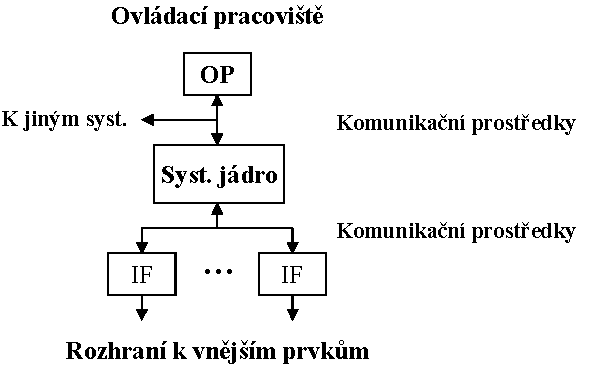
\includegraphics[width=0.8\linewidth]{zzt_fig003.pdf}
    \caption{Stanice
             (\cite[s.~11]{Chudacek2005})}
    \label{zzt:fig003}
  \end{figure}


  \section{Klasifikace poruch}
    \textbf{Chyba} je rozdíl mezi správnou a skutečnou hodnotou nějaké veličiny. V zařízení se 
    chyby mohou obecně objevit jako \emph{důsledek (projev) poruchy některé jeho součásti, 
    působením nějakého cizího vlivu} nebo \emph{selháním lidského činitele}. Za poruchy hardware se 
    považují všechna vybočení z předpokládaných vlastností stavebního prvku (součástky, dílu) 
    zařízení. Předpokládanými vlastnostmi prvků přitom jsou vlastnosti odpovídající příslušným 
    technickým podmínkám popisujícím jeho vlastnosti. Jako omyl lze označit každou lidskou činnost, 
    která může vést k nezamýšlenému chování zařízení. V širším slova smyslu se jako 
    \textbf{porucha} označují souhrnně všechny příčiny vedoucí k chybě, tj. poruch součásti, 
    cizí vliv i omyl.

%~~~~~~~~~~~~~~~~~~~~~~~~~~~~~~~~~~~~~~~~~~~~~~~~~~~~~~~~~~~~~~~~~~~~~~~~~~~~~~~~~~~~~~~~~~~~~~~~~~
\printbibliography[title={Seznam literatury}, heading=subbibliography]
\addcontentsline{toc}{section}{Seznam literatury}

\chapter{Bezpečnost a spolehlivost zabezpečovacích systémů}
 \section{Spolehlivost}
 \section{Bezpečnost}
    V různých publikacích je možné najít různé definice bezpečnosti. Například norma 
    EN~61508\footnote{Funkční bezpečnost elektrických/elektronických/programovatelných 
    elektronických systémů souvisejících s bezpečností (Functional safety of electrical/ 
    electronic/programmable electronic systems), obecná norma funkční bezpečnosti, která se opírá o 
    dvě základní koncepce - životní cyklus bezpečnosti a úroveň integrity bezpečnosti 
    (\texttt{SIL})} 
    definuje bezpečnost jako nepřítomnost netolerovaného rizika. Z této definice je zřejmé, že 
    bezpečnost je úzce spjatá s rizikem, a je nutné bezpečnost třeba chápat relativně. Když se 
    řekne, že řídicí systém je bezpečný, neznamená to jeho absolutní bezpečnost (ta je prakticky 
    nedosažitelná vzhledem na existenci objektivních faktorů, jako je například úroveň poznání, 
    technologická úroveň a limitované finanční prostředky), ale taková úroveň bezpečnosti, 
    která zodpovídá definovaným bezpečnostním požadavkům na tento řídicí systém. 

    Relativnost v pojímání bezpečnosti znamená posun od kvalitativního ke kvantitativnímu chápaní bezpečnosti.

    Kvalitativně je bezpečnost chápána jako schopnost řídicího systému zajistit omezení důsledků 
    poruch řídicích systému v daných podmínkách a v daném časovém intervalu. Matematicky je možné 
    kvalitativní bezpečnost řídicího systému vyjádřit jako 
    \begin{equation}
      E_H = 0,
    \end{equation}
    kde \(E_H\) je množina nebezpečných stavů, které jsou důsledkem výskytu pravděpodobných poruch 
    řídicího systému. Pravděpodobná porucha je taková porucha z množiny všech poruch, jejichž 
    výskyt během provozu řídicího systému je nutné předpokládat (vzhledem na požadovanou úroveň 
    bezpečnosti řídicího systému).
	
    Kvantitativně je bezpečnost řídicího systému chápána jako pravděpodobnost nepřítomnosti
    jakéhokoliv nebezpečného stavu v řídicím systému v daných podmínkách a v daném časovém
    intervalu. Je zřejmé, že i když pravděpodobnost nebezpečného stavu řídicího je malá, neznamená
    to, že se nebezpečný stav nemůže vyskytnou v nejbližším časovém intervalu, Matematicky je možné
    kvantitativní bezpečnost vyjádřit tak, že
    \begin{equation}
      P_{HT}(t)\geq P_{HT}(t)>0,
    \end{equation}
    kde \(P_{HT}(t)\) je pravděpodobnost tolerovaného nebezpeční řídicího systému a \(P_{HR}(t)\)
    je reálná pravděpodobnost nebezpeč\-ného stavu řídicího systému.
	 
    Na kvantitativním hodnocení bezpečnosti řídicího systému je v podstatě možné uplatnit stejné 
    teoretické postupy, jako při hodnocení spolehlivosti technických systémů. Zásadní rozdíl je v 
    tom, že při hodnocení spolehlivosti standardních řídicích systémů se obvykle rozlišují dva 
    stavy - bezporuchový stav a poruchový stav, a k těmto dvěma stavům se vztahují také 
    kvantitativní ukazatele spolehlivosti. Při hodnocení bezpečnosti řídicích systémů musíme 
    uvažovat s dvěma druhy poruchových stavů - bezpečným a nebezpečným poruchovým stavem. 
    Bezpečnost řídicího systému se potom vyjadřuje pomocí ukazatelů bezpečnosti (například 
    pravděpodobnost výskytu nebezpečné poruchy, intenzita nebezpečných poruch, ...).

    Při kvantitativním hodnocení důsledků poruch na bezpečnost řídicího systému se obvykle k 
    hodnoceným řídicím systémům přistupuje jako k neobnovovaným objektům, protože z pohledu 
    bezpečnosti jsou důležité dva stavy (bezpečný, nebezpečný) a analýza končí výskytem nebezpečné 
    poruchy (může jít o jednu poruchu, nebo o kombinaci více poruch, které nejsou individuálně 
    nebezpečné). To znamená, že od uvedení řídicího systému do provozu, až po výskyt nebezpečné 
    poruchy, se může řídicí systém střídavě nacházet ve funkčním, nebo nefunkčním stavu (nefunkční 
    ještě neznamená nebezpečný). Z tohoto důvodu ukazatele bezpečnosti jsou podobné ukazatelům 
    bezporuchovosti neobnovovaných objektů. 
  
    \subsection{Základní legislativa}
      \begin{itemize}
        \item \textbf{EN 61508} - \emph{základní všeobecná norma pro SRCS}; pojednává o funkční
              bezpečnosti elektrických/elektronických/programovatelných elektronických systémů
              souvisejících s bezpečností (Functional safety of electrical/electronic/programmable
              electronic systems), obecná norma funkční bezpečnosti, která se opírá o dvě základní
              koncepce - životní cyklus bezpečnosti a úroveň integrity bezpečnosti (\texttt{SIL})
              \begin{itemize}
                \item EN 61508-1: Všeobecné požadavky
                \item EN 61508-2: Požadavky na elektrické / elektronické / programovatelné
                                  elektronické systémy související s bezpečností
                \item EN 61508-3: Požadavky na SW
                \item EN 61508-4: Definice a zkratky
                \item EN 61508-5: Příklady metod určování úrovně integrity bezpečnosti
                \item EN 61508-6: Metodické pokyny na používání EN 61508-2, STN EN 61508-3
                \item EN 61508-7: Přehled technik a opatření
              \end{itemize}
        \item \textbf{EN 50126}: Railway applications – The specification and demonstration of
              reliability, availability, maintainability and safety (RAMS)
              \begin{itemize}
                \item Part 1: Basic requirements and generic process. 1999
                \item Part 2: Guide to the application of EN 50126-1 for safety. 2007
                \item Part 3: Guide to the application of EN 50126-1 for rolling stock RAMS. 2008  
              \end{itemize}
              Zabývá se specifikací parametrů RAMS (spolehlivost, pohotovost, udržovatelnost,
              a bezpečnost) obecně pro všechny železniční systémy, reaguje na skutečnost, že
              naléhavost požadavků na bezpečnost funkce jednotlivých železničních systémů je různá
              a lze je tedy splňovat s různou pravděpodobností jejich selhání. Také zavádí pojem
              \emph{integrita bezpečnosti (safety integrity - celistvost, úplnost, neporušenost
              bezpečnosti)}, který definuje jako pravděpodobnost, s níž systém uspokojivě splní
              požadované bezpečnostní funkce, za všech stanovených podmínek a ve stanoveném časovém
              období. Jde o to, do jaké míry může být pro bezpečnost relevantní funkce narušena
              např. poruchami vlastního zařízení, omyly obsluhy, vnějším rušením atd.
        \item \textbf{EN 50128}: Railway applications – Communication, signalling and processing
              systems – Software for railway control and protection systems. 2003          
        \item \textbf{EN 50129}: Railway applications – Communication, signalling and processing
              systems – Safety-related electronic systems for signalling. 2011
              Modifikovaně byl pojem integrita bezpečnosti přenesen i do této normy pro železniční
              zabezpečovací systémy. I klasická zabezpečovací technika bez velkého zdůrazňování
              respektovala, že nejsou na všechna zařízení kladeny stejně důrazné bezpečnostní
              požadavky (kategorie zařízení, vedlejší tratě/hlavní tratě, zařízení pro ČD/zařízení
              pro vlečky, staniční zařízení/spádoviště atd.). Uvidíme dále, že pojmu integrita
              bezpečnosti je pro zabezpečovací zařízení dominantně obsažena oblast, kterou běžně v
              této technice označujeme(a také normá EN 50129 ji tak označuje ve své základní části)
              termínem technická bezpečnost. Úvahy okolo integrity bezpečnosti zde sledujeme
              odděleně od úvah o technické bezpečnosti (přes jejich podobnost) pro jejich výhodnost
              zejména v úvodních fázích projektu nového systému (zařízení, výrobku, atd.)
        \item \textbf{EN 50159: Railway applications – Communication, signalling and processing
              systems - Safety-related communication in transmission systems. 2010}            
      \end{itemize}
    
      Vyjmenované normy se poněkud liší v definici termínu \emph{bezpečnost}:  
      \begin{itemize}
        \item Bezpečnost (Safety) – nepřítomnost nepřijatelných úrovní rizika poškození (EN50129)
        \item Bezpečnost (Safety) – nepřítomnost nepřijatelného rizika. (EN61508)
        \item Bezpečnost při poruše (Fail Safe) – vlastnost konstrukce objektu zabraňující,
              aby jeho poruchy způsobili nebezpečné poruchové stavy. (IEC 50 (191))
        \item Kvalitativní bezpečnost – schopnost systému zajistit omezení důsledku poruch
              systému v daných podmínkách a v daném časovém intervale.
        \item Kvantitativní bezpečnost – pravděpodobnost nepřítomnosti jakéhokoliv
              nebezpečného stavu v systéme v daných podmínkách a v daném časovém intervale.
      \end{itemize}

    \subsection{Ukazatel bezpečnosti}
      \fbox{Pravděpodobnost bezpečného provozu} je pravděpodobnost, že objekt může bezpečně plnit 
      požadovanou funkci v daných podmínkách v časovém intervalu \(t_1,\, t_2\).
      \begin{equation}
        R_S(t_1,\, t_2) = 1- F_H(t_1,\, t_2),
      \end{equation}
      kde \(F_H(t_1,\, t_2)\) je distribuční funkce, která naopak vyjadřuje pravděpodobnost, že
      objekt nemůže bezpečně plnit požadovanou funkci k daným podmínkám v časovém intervalu
      \(t_1,\, t_2\).
      \begin{equation}
        F_H(t_1,\, t_2) = \int_{t_1}^{t_2}f_H(t)\cdot\dd{t},
      \end{equation}
      kde \(f_H(t)\) je hustota pravděpodobnosti nebezpečné poruchy objektu. 

      \fbox{Intenzita nebezpečných poruch} \(\lambda_H(t)\) definujme jako limitu poměru podmíněné
      pravděpodobnosti, že časový okamžik vzniku nebezpečné poruchy objektu \(T\) padne do daného
      časového intervalu \(t,\, t+\Delta t\), přičemž délka časového intervalu \(\Delta
      t\rightarrow0\)
      \begin{equation}\label{DZT:eq_def_lambdaH}
        \lambda_H=\frac{f_H(t)}{R_S(t)}.
      \end{equation}

      Protože nebezpečné poruchy jsou méně časté, zkoušky na určení požadovaných ukazatelů
      bezpečnosti by bylo třeba provádět dlouhodobě, což je prakticky nemožné. 
    
  \section{Integrita bezpečnosti}
    Všeobecně je možné konstatovat, že SRCS realizuje řídící i ochranné funkce (obr.
    \ref{DZT:fig_DZT_SRCS_fce}). Jelikož selhání řídicí funkce může způsobit ohrožení bezpečnosti,
    je třeba i tyto funkce považovat za bezpečnostní.
    \begin{figure}[hb!]
      \centering
      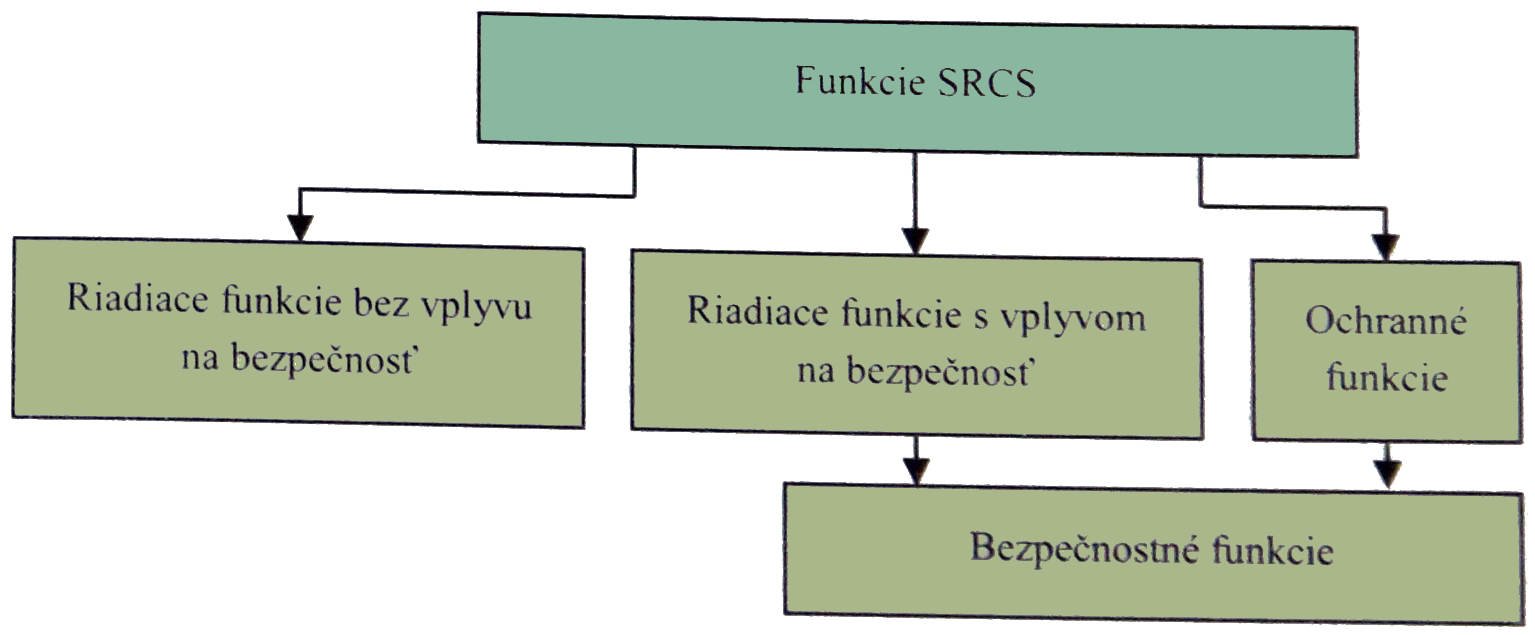
\includegraphics[width=1\linewidth]{DZT_SRCS_fce.jpg}
      \caption{Vztah mezi bezpečnostními funkcemi a moduly SRCS}
      \label{DZT:fig_DZT_SRCS_fce}
    \end{figure}    
    Bezpečnostní funkce jsou definované na základě analýzy rizik jako technická opatření na snížení
    rizika spojeného s konkrétními nebezpečí na tolerovatelnou úroveň. Účinnost bezpečnostní funkce
    se určuje pomocí úrovně integrity bezpečnosti \emph{(\texttt{SIL} - safety integrity level)}. 
    
    Norma \emph{EN 61508} definuje integritu bezpečnosti jako pravděpodobnost, že SRCS bude plnit 
    požadované bezpečné funkce za všech stanovených podmínek v rámci stanoveného operačního 
    prostředí a během stanoveného časového období. Všeobecně lze konstatovat, že čím je integrita
    bezpečnosti SRCS větší, tím je menší pravděpodobnost selhání bezpečností funkce realizovaných
    SRCS.  
    
    Integrita bezpečnosti se skládá ze dvou částí a to:
    \begin{itemize}
      \item \emph{integrity bezpečnosti proti systematickým poruchám}: jde o nekvantifikovatelnou
            část integrity bezpečnosti, která souvisí s nebezpečnými systematickými poruchami 
            hardware a software; integrity bezpečnosti proti systematickým poruchám se dosahuje
            především opatřeními na předcházení chybám a poruchám; vzhledem k tomu, že jde o 
            nekvantifikovatelnou část integrity bezpečnosti, je vhodnější chápat integritu 
            bezpečnosti jako vlastnost a né jako pravděpodobnost; hodnocení integrity bezpečnosti
            proti systematickým chybám a poruchám se realizuje kontrolou dodržování opatření
            předcházejících chybám a poruchám, mezi které patří také důsledné testování korektní
            realizace bezpečnostních funkcí; 
      \item \emph{integrity bezpečnosti proti náhodným poruchám}: jde o kvantifikovatelnou část
            integrity bezpečnosti, která se týká náhodných poruch hardware vyplývajících z konečné
            bezporuchovosti použitých součástek; hodnocení integrity bezpečnosti proti náhodným
            poruchám se realizuje prostřednictvím pravděpodobnostních výpočtů.
    \end{itemize}
    
    Aby se dosáhla požadovaná integrita bezpečnosti, musí být splněné požadavky na integritu proti 
    systematickým poruchám i náhodným poruchám. 
    
    \subsection{Úroveň integrity bezpečnosti}
      Úroveň integrity bezpečnosti (\emph{Safety Integrity Levels - \texttt{SIL}}) se dělí podle EN 
      50129
      do čtyř kategorií - úroveň 4 (\texttt{SIL} 4) je nejvyšší, úroveň 1 (\texttt{SIL} 1) je 
      nejnižší.  Pokud se
      objevuje úroveň \texttt{SIL} 0, značí to, že se jedná o systém na které nejsou kladeny žádné
      bezpečnostní požadavky (ve smyslu zabezpečovací techniky)
      
      Proto, aby SRCS mohl být zařazen do odpovídající úrovně bezpečnosti \texttt{SIL}, musí 
      vyhovovat
      těmto faktorům:
      \begin{itemize}
        \item naplnění podmínek řízení kvality, 
        \item naplnění podmínek řízené bezpečnosti,
        \item splnění požadavků na technickou bezpečnost, 
        \item dosažení kvantitativního cíle
      \end{itemize}
      
      Jak patrno, splnění kvantitativního ukazatele samo o sobě neznamená, že bylo dosaženo
      odpovídající úrovně bezpečnosti. To platí ovšem i naopak - splnění tří předchozích podmínek
      (řízení kvality, řízení bezpečnosti a technické bezpečnosti) nezaručuje, že bylo dosaženo
      kvantitativních cílů a nelze tedy tvrdit, že zařízení lze zařadit do odpovídající skupiny
      \texttt{SIL} (\ref{DZT:fig_EN50129_SIL_techniques}).
      
      \begin{figure}[ht!]% Relationship between \texttt{SIL}s and techniques
        \centering
        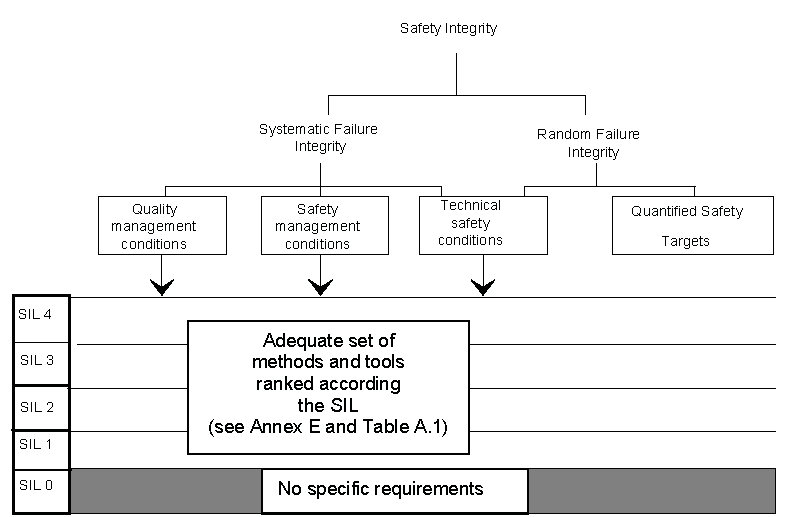
\includegraphics[width=0.95\linewidth]{EN50129_SIL_techniques.pdf}
        \caption{Vztah mezi \texttt{SIL} úrovní a technikami jejich dosažení}
        \label{DZT:fig_EN50129_SIL_techniques}
      \end{figure}
      
      Žádná z norem \texttt{CENELEC} nepředepisuje, které zařízení musí být jaké úrovně. Toto 
      určení je 
      ponecháno na provozovateli, resp. regulátorovi, vyplyne také z provedených analýz rizik 
      a hazardů.
      
      Následující tabulka shrnuje definované úrovně integrity bezpečnosti a zároveň dává do
      souvislosti s tolerovatelnými četnostmi hazardů. \texttt{SIL} jsou tedy prostředkem přiřazení
      kvalitativních přístupů (pro vyloučení systematických poruch) ke kvantitativnímu přístupu
      (pro řízení náhodných poruch), neboť systematické poruchy nelze kvantifikovat.
      \begin{table}[h]
        \centering
        \begin{tabular}{|c|c|}
          \hline
           Úroveň integrity &  Tolerovatelná četnost hazardu            \\
             bezpečnosti \texttt{SIL} &  THR [za hodinu a funkci]       \\ \hline\hline 
              4        & \(10^{-9}\leq THR < 10^{-8}\)                  \\ \hline
              3        & \(10^{-8}\leq THR < 10^{-7}\)                  \\ \hline
              2        & \(10^{-7}\leq THR < 10^{-6}\)                  \\ \hline
              1        & \(10^{-6}\leq THR < 10^{-5}\)                  \\ \hline
        \end{tabular}
        \caption{\texttt{SIL} tabulka: Funkce, jejichž kvantitativní požadavky by převyšovaly 
                 hranici \(10^{-9}\), která se zdánlivě nelogicky objevuje u \texttt{SIL4}, vyžaduje
                 podle normy \texttt{EN~50129} zvláštní technická nebo provozní opatření pro 
                 dosažení tak mimořádného cíle.}
      \end{table}
       
      \begin{enumerate}
        \item Z normy jasně vyplývá rozdělení na dvě skupiny \texttt{SIL 1,2} vs. \texttt{SIL 3,4}, 
              u nichž je výrazný rozdíl v požadavcích, které je potřeba splnit, aby SRCS mohl 
              patřit do dané skupiny. To je velmi dobře patrné z tabulek v příloze \texttt{E} normy 
              \texttt{EN 50129}, která se zabývá technikami a opatřeními pro řízení náhodných a 
              systematických poruch. 
        \item Druhým důležitým faktem je poněkud odlišná definice chápání úrovní \texttt{SIL} v 
              EN~61508. \emph{Funkční bezpečnost elektrických, elektronických, programovatelných
              elektronických systémů souvisejících s bezpečností}. Tato norma je obecnou normou pro
              průmyslové elektronické systémy, z níž vycházejí normy EN~50126, EN 50~129 atd.
              jakožto specifické normy pro železniční aplikace. Důležitou odlišností ve specifikaci
              \texttt{SIL}, viz tab. 2 a 3 v první části této normy (EN~61508-1). Nicméně tabulka 3 
              pro
              režim provozu s vysokým, resp. nepřetržitým vyžádáním odpovídá tabulce v normě
              EN~50129. Avšak i pro tyto systémy se zde jeví určitá odlišnost v požadavcích na
              zajištění dané \texttt{SIL}. Norma EN~61508 je zaměřena pouze na \emph{funkční 
              bezpečnost},
              není zde zahrnutý požadavek na bezpečnou reakci na ojedinělé náhodné poruchy. S
              poruchami se samozřejmě pracuje, mají být provedena opatření k jejich maximálnímu
              potlačení - četnosti i následku, nicméně může stačit, když systém je schopen poruchy
              detekovat a dát o nich vědět (např. obsluze). Závěrem nutno dodat, že je potřeba
              určité obezřetnosti k tvrzení, že systém splňuje daný \texttt{SIL}. Tento údaj musí 
              být
              doplněn specifikací, která norma byla při klasifikaci použita.
      \end{enumerate}
      
%\end{Czech}

%} %tikzset
%~~~~~~~~~~~~~~~~~~~~~~~~~~~~~~~~~~~~~~~~~~~~~~~~~~~~~~~~~~~~~~~~~~~~~~~~~~~~~~~~~~~~~~~~~~~~~~~~~~
\printbibliography[title={Seznam literatury}, heading=subbibliography]
\addcontentsline{toc}{section}{Seznam literatury}
} % DEBUG was off

%==================================================================================================
\setpartpreamble[u]{
\begin{center}
  \vspace{1cm}
  \Huge \uppercase{\textbf{Prvky}} \\
  \Huge \uppercase{\textbf{Železniční techniky}} \\
  \vspace{2cm}
  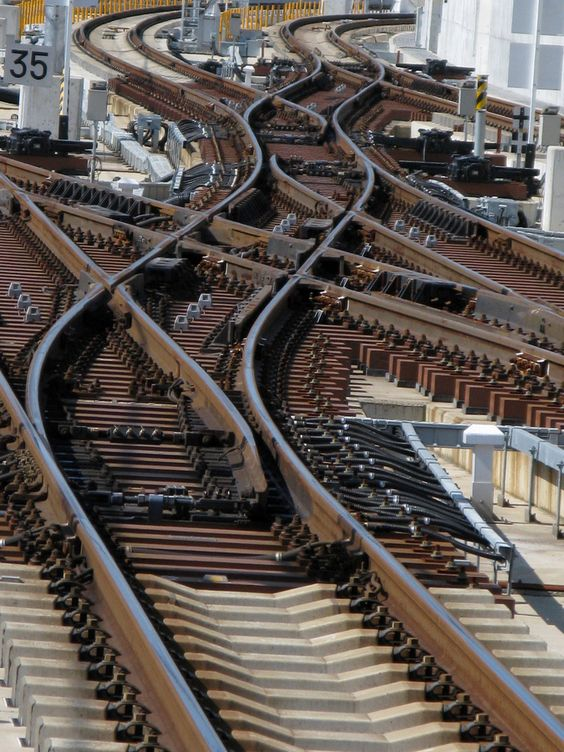
\includegraphics[width=0.8\linewidth]{PZT.jpg}
\end{center}
}

\part{PZT}\label{part:PZT}
\parttoc

\ifthenelse{ \equal{\DebugMode}{true} }{
% Debug mode ON
  % !TeX spellcheck = cs_CZ
%{\tikzset{external/prefix={tikz/PZT/}}
% \tikzset{external/figure name/.add={ch01_}{}}
%---------------------------------------------------------------------------------------------------
% file ra3ch001.tex
%---------------------------------------------------------------------------------------------------
%====================Kapitola: Výhybky =============================================================
\chapter{Výhybka}\label{pzt:chapI}
\minitoc

%} %tikzset
%~~~~~~~~~~~~~~~~~~~~~~~~~~~~~~~~~~~~~~~~~~~~~~~~~~~~~~~~~~~~~~~~~~~~~~~~~~~~~~~~~~~~~~~~~~~~~~~~~~
\printbibliography[title={Seznam literatury}, heading=subbibliography]
\addcontentsline{toc}{section}{Seznam literatury}

  % !TeX spellcheck = cs_CZ
%{\tikzset{external/prefix={tikz/PZT/}}
% \tikzset{external/figure name/.add={ch02_}{}}
%---------------------------------------------------------------------------------------------------
% file ra3ch001.tex
%---------------------------------------------------------------------------------------------------
%====================Kapitola: Detekce kolejových vozidel ==========================================
\chapter{Detekce kolejových vozidel}\label{pzt:chapII}
\minitoc

%} %tikzset
%~~~~~~~~~~~~~~~~~~~~~~~~~~~~~~~~~~~~~~~~~~~~~~~~~~~~~~~~~~~~~~~~~~~~~~~~~~~~~~~~~~~~~~~~~~~~~~~~~~
\printbibliography[title={Seznam literatury}, heading=subbibliography]
\addcontentsline{toc}{section}{Seznam literatury}

  % !TeX spellcheck = cs_CZ
%{\tikzset{external/prefix={tikz/PZT/}}
% \tikzset{external/figure name/.add={ch03_}{}}
%---------------------------------------------------------------------------------------------------
% file ra3ch001.tex
%---------------------------------------------------------------------------------------------------
%====================Kapitola: Detekce kolejových vozidel ==========================================
\chapter{Návěstidlo}\label{pzt:chapIII}
\minitoc
%} %tikzset
%~~~~~~~~~~~~~~~~~~~~~~~~~~~~~~~~~~~~~~~~~~~~~~~~~~~~~~~~~~~~~~~~~~~~~~~~~~~~~~~~~~~~~~~~~~~~~~~~~~
\printbibliography[title={Seznam literatury}, heading=subbibliography]
\addcontentsline{toc}{section}{Seznam literatury}

}
{
 % DEBUG was off
%========== Kapitola 001: Bezpečnost a spolehlivost zabezpečovacích systémů =======================
%  % !TeX spellcheck = cs_CZ
%{\tikzset{external/prefix={tikz/PZT/}}
% \tikzset{external/figure name/.add={ch01_}{}}
%---------------------------------------------------------------------------------------------------
% file ra3ch001.tex
%---------------------------------------------------------------------------------------------------
%====================Kapitola: Výhybky =============================================================
\chapter{Výhybka}\label{pzt:chapI}
\minitoc

%} %tikzset
%~~~~~~~~~~~~~~~~~~~~~~~~~~~~~~~~~~~~~~~~~~~~~~~~~~~~~~~~~~~~~~~~~~~~~~~~~~~~~~~~~~~~~~~~~~~~~~~~~~
\printbibliography[title={Seznam literatury}, heading=subbibliography]
\addcontentsline{toc}{section}{Seznam literatury}

%  % !TeX spellcheck = cs_CZ
%{\tikzset{external/prefix={tikz/PZT/}}
% \tikzset{external/figure name/.add={ch02_}{}}
%---------------------------------------------------------------------------------------------------
% file ra3ch001.tex
%---------------------------------------------------------------------------------------------------
%====================Kapitola: Detekce kolejových vozidel ==========================================
\chapter{Detekce kolejových vozidel}\label{pzt:chapII}
\minitoc

%} %tikzset
%~~~~~~~~~~~~~~~~~~~~~~~~~~~~~~~~~~~~~~~~~~~~~~~~~~~~~~~~~~~~~~~~~~~~~~~~~~~~~~~~~~~~~~~~~~~~~~~~~~
\printbibliography[title={Seznam literatury}, heading=subbibliography]
\addcontentsline{toc}{section}{Seznam literatury}

%  % !TeX spellcheck = cs_CZ
%{\tikzset{external/prefix={tikz/PZT/}}
% \tikzset{external/figure name/.add={ch03_}{}}
%---------------------------------------------------------------------------------------------------
% file ra3ch001.tex
%---------------------------------------------------------------------------------------------------
%====================Kapitola: Detekce kolejových vozidel ==========================================
\chapter{Návěstidlo}\label{pzt:chapIII}
\minitoc
%} %tikzset
%~~~~~~~~~~~~~~~~~~~~~~~~~~~~~~~~~~~~~~~~~~~~~~~~~~~~~~~~~~~~~~~~~~~~~~~~~~~~~~~~~~~~~~~~~~~~~~~~~~
\printbibliography[title={Seznam literatury}, heading=subbibliography]
\addcontentsline{toc}{section}{Seznam literatury}

} % DEBUG was off

%%==================================================================================================
%\part{MOL}\label{part:MOL}
%\parttoc
%
%\ifthenelse{ \equal{\DebugMode}{true} }{
%% Debug mode ON
%%  \input{../src/ZZT/chap/ra2ch001.tex}
%}
%{
% % DEBUG was off
%%========== Kapitola 001: Bezpečnost a spolehlivost zabezpečovacích systémů =======================
%%  \input{../src/ZZT/chap/ra2ch001.tex}
%} % DEBUG was off

%==================================================================================================
%    %===================================================================================================
% Německý jazyk
% NJ.tex
%===================================================================================================
% notes:
%~~~~~~~~~
%---------------------------------------------------------------------------------------------------
% Setting path to image 
  \graphicspath{{../src/NJ/img/}}
  \renewcommand\arraystretch{0.6} \setlength\minrowclearance{2.4pt}
  \setlength{\belowcaptionskip}{-3em}
%========================== Kapitola 1 =============================================================
\LuaPartBckgrnd{titleBG_fractal1.png}
\LuaPartTitle{NJI}{Německý jazyk}{NJI}
\parttoc

\ifthenelse{ \equal{\DebugMode}{true} }{
% Debug mode ON
}
{
% DEBUG was off
  % !TeX spellcheck = cs_CZ
%================ Kapitola 1: Sie sind aber neugierig! =============================================
% \let\cleardoublepage\clearpage  % remove blank pages coming between two chapters 
\chapter{Lektion 1: Sie sind aber neugierig!}\label{NJ:chap_N1_L1}

\section*{Slovní zásoba}
  Ve slovníčku se užívají zkrácené tvary členu: \textbf{der} \(\rightarrow\) r, \textbf{die} 
  \(\rightarrow\) e, \textbf{das} \(\rightarrow\) s.  
  
  \begin{widetext}
%  \begin{table}[ht!]   % L1_Wortschatz01.jpg
    \centering
    \begin{tabular}{llll}
      \hline
      aber        & ale               & was               & co                                \\
      neugierig   & zvědavý, -ě       & machen            & dělat                             \\
      wie         & jak, jako, jaký   & hier              & zde, tady                         \\
      hei{\ss}en  & jmenovat se       & fahren            & jet                               \\
      bitten      & prosit            & e Universit{\"a}t & univerzita                        \\
      und         & a                 & auch              & také, i                           \\
      woher       & odkud             & e Straßenbahn     & tramvaj                           \\
      kommen      & přijet, přicházet & begleiten         & doprovodit, doprovázet            \\
      aus         & z                 & dich              & tě, tebe                          \\
      (s) M{\"u}nchen  & Mnichov      & nat{\"u}rlich     & přirozeně, -ě,                    \\
                  &                   &                   & samozřejmě                        \\
      freuen      & (po)těšit         & noch              & jestě                             \\
      mich        & mě, mne           & r Freund          & přítel                            \\
      (s) Prag    & Praha             & studieren         & studovat                          \\
      nein        & ne, nikoli        & eigentlich        & vlastně                           \\
      wo          & kde               & e Geschichte      & dějiny, dějepis,                  \\
                  &                   &                   & historie, příběh                  \\
      liegen      & ležet; být        & e Schule          & škola                             \\
      weit        & daleko            & besuchen          & navštívit, navštěvovat            \\
      von         & od, z, o          & r Name            & jméno                             \\
      von hier    & odtud             & wohnen            & bydlet                            \\
      ja          & ano               & in                & v, do, za (časově)                \\
      ziemlich    & dost, značný, -ě  & (s) Graz          & Štýrskě Hradec                    \\
      gehen       & jít, chodit       & sagen             & říci, říkat                       \\
      wer         & kdo               & mein, meine, mein & můj, má, mé‚                      \\
      e Frau      & paní, slečna      & e Stadt           & město                             \\
      dort        & tam               & kennen            & znát                              \\
      doch        & přece             & sehr              & velmi                             \\
      danken      & (po)děkovat       & sch{\"o}n         & pěkný, -ě                         \\
      gut         & dobrý, dobře      & s M{\"a}dchen     & dívka, děvče \\
      \hline
    \end{tabular}
%    \caption*{ }
%  \end{table}
  \end{widetext}
  
  \subsection*{Vazby}
    \begin{table}[ht!]   % L1_Redensart01.jpg
      \begin{tabular}{ll}
        bitte                      & prosím                     \\
        Woher kommen Sie?          & Odkud jste?                \\
        Das stimmt.                & To je pravda. To souhlasí  \\
        Verzeihung!                & Promiňte!                  \\
        (Es) freut mich!           & Těší mě!                   \\
        Wo liegt es?               & Kde to je?                 \\
        danke                      & děkuji                     \\
        Wie gehťs? (Wie geht es?)  & Jak se daří?               \\
        Ich fahre zur Universität. & Jedu na univerzitu.        \\
        Ich gehe zur Straßenbahn   & Jdu na tramvaj.            \\
        Darf ich?                  & Smím? / Mohu?              \\
        Er geht zur Schule.        & Chodí/ jde do školy. 
      \end{tabular}
      \caption*{ }
    \end{table}


\section*{Gramatika}
  \subsection*{Osobní zájména v 1. pádě}
    \begin{table}[ht!]   % L1_Grammatik01.jpg
      \begin{tabular}{lllll}
        \hline
              & \multicolumn{2}{l}{\texttt{j. č.}}
              & \multicolumn{2}{l}{\texttt{mn. č.}}     \\  
        \hline
        1.os. & ich & já  & wir & my          \\
        2.os. & du  & ty  & ihr & vy          \\
        3.os. & er  & on  & sie & oni         \\
              & sie & ona & Sie & vy (vykání) \\
              & es  & ono &     &             \\
        \hline
      \end{tabular}
      \caption*{ }
    \end{table}
    Při \emph{vykání} jedné nebo více osobám se používá \emph{3. osoby množného čísla}, tedy 
    zájmena \emph{Sie}, které se píše \emph{vždy} s velkým písmenem.
          
  \subsection*{Časování pravidelných sloves v přítomném čase}
    \begin{table}[ht!]   % L1_Grammatik01.jpg
      \begin{tabular}{llll}
        \hline
        \multicolumn{4}{c}{\texttt{machen \(\rightarrow\) dělat}}     \\
        \hline
        ich mache & dělám & wir machen & děláme  \\
        du machst & děláš & ihr macht  & děláte  \\
        er macht  & dělá  & sie machen & dělají  \\
        sie macht & dělá  & Sie machen & děláte  \\
        es macht  & dělá  &            &         \\
        \hline
      \end{tabular}
      \caption*{ }
    \end{table}

    \begin{table}[ht!]   % L1_Grammatik01.jpg
      \begin{tabular}{llll}
        \hline
        \multicolumn{4}{c}{\texttt{begleiten \(\rightarrow\) doprovázet}}     \\
        \hline   
        ich begleite    & doprovázím & wir begleiten  & doprovázíme \\
        du begleitest   & doprovázíš & ihr begleitet  & doprovázíte \\
        er begleitet    & doprovází  & sie begleiten  & doprovázejí \\
        sie begleitet   & doprovází  & Sie begleiten  & doprovázíte \\
        es begleitet    & doprovází  &                &             \\ 
        \hline
      \end{tabular}
      \caption*{ }
    \end{table}
    
    Infinitiv slovesa končí převážně na \emph{-en}, jen v málo případech na \emph{-n}. Slovesný 
    kmen získáme odtržením infinitivní koncovky. Končí-li kmen na \emph{-t} (begleit-) nebo 
    \emph{-d}, vsouvá se pro snazší výslovnost mezi kmen a koncovku hláska \emph{-e-}, tj. v 2. a 
    3. osobě jednotného čísla a ve 2. osobě množného čísla: du begleitest, er begleitet, ihr 
    begleitet.

    U sloves, kde končí kmen na sykavku (hei{\ss}-), se přidává v 2. osobě jednotného čísla 
    pouze koncovka \emph{-t}. 2. a 3. osoba jednotného čísla pak mají shodný tvar: du hei{\ss}t, er 
    hei{\ss}t.
    
    Časujte ve všech osobách následující slovesa: \textbf{bitten} - prosit, \textbf{hei{\ss}en} - jmenovat se:  
    \begin{table}[ht!]   % 
      \begin{tabular}{llll}
        \hline
        \multicolumn{2}{c}{\texttt{bitten \(\rightarrow\) prosit}} & 
        \multicolumn{2}{c}{\texttt{hei{\ss}en \(\rightarrow\) jmenovat se}}     \\
        \hline   
        ich bitte         & wir bitten      & ich hei{\ss}e        & wir hei{\ss}en     \\
        du bittest        & ihr bittet      & du hei{\ss}t         & ihr hei{\ss}t      \\
        er/sie/es bittet  & sie/Sie bitten  & er/sie/es hei{\ss}t  & sie/Sie hei{\ss}en \\
        \hline
      \end{tabular}
      \caption*{ }
    \end{table}

  \subsection*{Časování slovesa „sein" (být)}
    \begin{table}[ht!]   % L1_Grammatik02.jpg
      \begin{tabular}{llll}
        \hline
          \multicolumn{2}{l}{\texttt{j. č.}}  & 
          \multicolumn{2}{l}{\texttt{mn. č.}}  \\  
        \hline
         ich bin  & jsem & wir sind & jsme          \\
         du  bist & jsi  & ihr seid & jste          \\
         er  ist  & je   & sie sind & jsou          \\
         sie ist  & je   & Sie sind & jste (vykání) \\
         es  ist  & je   &     &                    \\
        \hline
      \end{tabular}
      \caption*{ }
    \end{table}
    
    Ich \underline{bin} Gabi. Er \underline{ist} Rolf. Wir \underline{sind} in Prag. Sie 
    \underline{sind} in Berlin. Du \underline{bist} Heike. Ihr \underline{seid} in Brno. Sie 
    \underline{sind} hier. 


  \subsection*{Člen a podstatné jméno v 1. pádě}
    \begin{table}[ht!]   % L1_Grammatik03.jpg
      \begin{tabular}{ll}
        Dort ist eine Frau.          & Tam je nějaká paní. \\
        Die Frau heißt Jutta Klein.  & Ta paní se jmenuje Jutta Kleinová.   \\
      \end{tabular}
      \caption*{ }
    \end{table}
    \begin{itemize}\addtolength{\itemsep}{-0.5\baselineskip}
      \item \textbf{Člen určitý} označuje věci známé nebo již zmíněné; do češtiny jej lze někdy 
            přeložit ukazovacím zájmenem „ten, ta, to".
      \item \textbf{Člen neurčitý} označuje věci neznámé, dosud nezmíněné; do češtiny jej lze 
            někdy přeložit neurčitým zájmenem „nějaký", případně číslovkou „jeden".
    \end{itemize}

    Podstatná jména se v němčině používají zpravidla se členem a píší se vždy velkým písmenem. 
    \textbf{Rod podstatných jmen} bývá často od češtiny odlišný: die Stadt - město, der Name - 
    jméno, das M{\"a}dchen - dívka atd.
    \begin{itemize}\addtolength{\itemsep}{-0.5\baselineskip} % L1_Grammatik04
      \item Ich heiße Marek. Sind Sie aus Prag?
      \item Das ist Frau Sommer. Ich studiere Medizin.
    \end{itemize}
    U podstatných jmen se někdy člen vynechává. Je to např. před osobními jmény, tituly, názvy 
    měst, u oborů studia apod. a v některých ustálených vazbách. Na tato podstatná jména je 
    průběžně upozorňováno jednak v gramatice, jednak u vazeb.

  \subsection*{Pořádek slov ve větě}  %L1_Grammatik05.jpg
    \begin{enumerate}
       \item \textbf{Slovosled v oznamovací větě:}
             \begin{table}[ht!]   
               \hspace*{2em}
               \begin{tabular}{llll}
                 Er           & studiert & in Prag.        & Studuje v Praze.                  \\
                 Eva aus Köln & studiert & auch in Prag.   & Eva z Kolína studuje také v Praze.\\
                 In Prag      & studiert & sie Geschichte. & V Praze studuje historii.         \\
               \end{tabular}
               \caption*{ }
             \end{table}
             
            Sloveso stojí v německé oznamovací větě vždy jako \textbf{2. větný člen}. Oznamovací 
            věta může mít \emph{přímý} nebo \emph{nepřímý} pořádek slov:
            \begin{itemize}
             \item \textbf{Přímý pořádek}:\newline
                   \emph{Podmět - sloveso - ostatní větné členy}
             \item \textbf{Nepřímý pořádek}:\newline
                   \emph{Zdůrazněný větný člen - sloveso - podmět - ostatní větné členy} 
          \end{itemize}
      \item \textbf{Slovosled v tázací větě:}
        \begin{table}[ht!] 
          \hspace*{2em} 
          \begin{tabular}{llll}
            Was machst du hier?  & Co tady děláš? \\
            Sind Sie aus Prag?   & Jste z Prahy?  \\
          \end{tabular}
          \caption*{ }
        \end{table}
         
         V \textbf{doplňovací otázce} (otázka začínající tázacím zájmenem) stojí sloveso 
         rovněž jako 2. větný člen. Ve \textbf{zjišťovací otázce} (otázka, na kterou je možno 
         odpovědět ano nebo ne) stojí sloveso na začátku věty, pak následuje podmět a teprve za ním 
         ostatní větné členy.
    \end{enumerate}
  
  \newpage
  \subsection*{Cvičení}
    \begin{example}\textbf{Fill in the correct ending:}\newline
      Ich geh\textbf{e} in die Schule. - Er komm\textbf{t} aus Spanien. - Ihr lern\textbf{t} 
      Deutsch. - Wir sprech\textbf{en} Englisch. - Du schreib\textbf{st} einen Brief.
    \end{example}

    \begin{example}\textbf{Fill in the correct personal pronoun:}\newline
     \textbf{Ich} gehe nach Hause. - \textbf{Ihr} seid aus Italien. - \textbf{Sie} (die Frau) 
     hei{\ss}t Sabine. - \textbf{Du} wohnst in Berlin. - Meine Mutter und ich, \textbf{wir} lernen 
     Deutsch.     
    \end{example}
    
    \begin{example}\textbf{Fill in the correct verbform:}\newline
      Wir \textbf{sind} (sein) in Wien. - Ihr arbeitet (arbeiten) bei einer gro{\ss}en Firma. - 
      Herr M{\"u}ller, Sie \textbf{kommen} (kommen) aber sp{\"a}t. - Mein Bruder \textbf{lebt} 
      (leben) in M{\"u}nchen. - Ich \textbf{schreibe} (schreiben) ein Buch. 
l    \end{example}

    \begin{example}\textbf{Přeložte:}\newline
      Co tady děláš? \emph{Was machst du hier?} - Jak se jmenuješ? \emph{Wie hei{\ss}t du?} - Kde 
      vlastně bydlíte? \emph{Wo wohnen Sie eigentlich.} - Bydlíme tady. \emph{Wir wohnen hier}. - 
      Kde je paní Sommerová? \emph{Wo ist frau Sommerova?} - (Ona) je přece tady. \emph{Sie ist 
      doch hier} - Tady jste! \emph{Hier sind Sie ja!} - Co říkáte? \emph{Was sagen Sie?} - 
      Přijdete také? \emph{Kommen Sie auch?} - Jste velmi zvědavý \emph{Sie sind sehr neugierig}. - 
      To je pravda. \emph{Das stimmt} - Jdeš na tramvaj? Doprovodím tě. Smím? \emph{Gehst du zur 
      Straßenbahn? Ich begleite dich. Darf ich?} - Kdo je to? Můj přítel z Prahy.\emph{Wer ist das? 
      Mein Freund aus Prag.} -  Kde je (leží) Praha? Znají mě. Studují také historii. \emph{Wo 
      liegt Prag? Kennen Sie mich? Sie studieren auch Geschichte.}
    \end{example}
  % !TeX spellcheck = de_DE
%================ Kapitola 2: Unsere Familie ==============================================
\setchaptertoc
\chapter{Lektion 2: Unsere Familie}\label{NJ:chap_N1_L2}

    \textbf{Unsere Familie ist ziemlich groß}. Darf ich sie vorstellen? Mein Vater ist 53 
    Jahre 
    alt, er arbeitet als Techniker. Seine Arbeit ist interessant, er kommt aber oft spät nach 
    Hause. Er wandert gern und bastelt auch viel.
    
    \textbf{Meine Mutter ist 49}, sie ist von Beruf Verkäuferin. Ihre Arbeit ist schwer und zu 
    Hause hat sie auch viel zu tun. Sie ist sehr fleißig, sie schafft immer alles. Und ihr Hobby? 
    Sie näht und strickt gern und geht auch schwimmen. Ich habe zwei Geschwister - einen Bruder und 
    eine Schwester. Meine Schwester Jana ist schon 24.  Sie ist verheiratet und wohnt jetzt in 
    Brno. Sie bekommt bald ein Kind. Dann werde ich Tante und Martin Onkel.
    
    Wer ist Martin? Das ist doch mein Bruder. Er ist Schüler, er besucht eine Fachschule.   
    Natürlich ist er noch ledig, aber er hat schon eine Freundin. Sie ist ganz nett. Martin ist ein 
    bisschen zu dick1, aber er treibt aktiv Sport: er spielt Fußball und Tennis, manchmal auch 
    Basketball und Volleyball. Die Schule findet er langweilig. Er lernt zwar leicht, aber er ist 
    faul.
    
    Also, jetzt kennt ihr schon meine Familie. Nein, einen Augenblick, mich kennt ihr doch noch 
    nicht! Ich heiße Petra, bin 21 Jahre alt, klein, schlank, blond und studiere Psychologie.    
    Ich habe einen Freund, aber wir heiraten noch nicht. Wir haben nämlich keine Zeit. Ich glaube 
    auch, ich bin noch zu jung. Was meint ihr?

  \section*{Slovní zásoba}

    \begin{widetext}
     \centering
%    \begin{table}[ht!] % L2_Wortschatz01.jpg, L2_Wortschatz02.jpg 
      \begin{tabular}{llll}  
        \hline
          e Familie          & rodina                & groß            & velký                 \\
          r Vater            & otec                  & stricken        & plést                 \\
          s Jahr             & rok                   & schwimmen       & plavat                \\
          alt                & starý, staře          & die Geschwister & sourozenci            \\
          arbeiten (als)     & pracovat (jako)       & r Bruder        & bratr                 \\
          e Arbeit           & práce e               & Schwester       & sestra                \\
          interessant        & zajímavý, -ě          & schon           & už, již               \\
          oft                & často                 & verheiratet     & ženatý, vdaná         \\
          spät               & pozdě, pozdní         & jetzt           & teď, nyní             \\
          s Haus             & dům                   & bald            & brzy                  \\
          zu Hause           & doma                  & s Kind          & dítě                  \\
          nach Hause         & domů                  & werden          & stát se (čím)         \\
          wandern            & chodit na             & e Freundin      & přítelkyně,           \\ 
                             & pěší výlety           &                 & kamarádka             \\
          gern               & rád, -a, -o           & e Tante         & teta                  \\
          bastel             & kutit r               & Onkel           & strýc, strýček        \\
          viel               & mnoho                 & erst            & teprve (časově)       \\
          e Mutter           & matka r               & Schüler         & žák                   \\
          r Beruf            & povolání,             & e Fachschule    & střední odborná       \\
                             & zaměstnání            &                 & škola                 \\
          e Verkäuferin      & prodavačka            & ledig           & svobodný (neženatý)   \\
          schwer             & těžký, těžce          & bekommen        & dostat                \\
          dann               & potom, pak            & ein bisschen    & trochu                \\
          tun, ich tue       & činit, konat, dělat   & zu              & příliš                \\
          fleißig            & pilný, -ě             & dick            & tlustý, -ě            \\
          immer              & vždy, stále           & r Sport         & sport                 \\
          schaffen           & stihnout, dokázat     & Sport treiben   & sportovat             \\
          alles              & všechno               & spielen         & hrát (si)             \\
          nähen              & šít                   & ganz            & docela, celý          \\
          nett               & milý, -e              & manchmal        & někdy, občas          \\
          finden             & najít                 & vorstellen      & představit            \\
                             & shledávat (jakým)     & klein           & malý                  \\
          \hline 
          langweilig         & nudný, -ě             & schlank         & 
          štíhlý                \\
          lernen             & učit se               & heiraten (4.p.) & ženit se, vdávat 
          se,  \\
                             &                       &                 & brát se 
                             (si)          \\
          zwar               & sice                  & nämlich         & 
          totiž                 \\
          leicht             & lehký, lehce          & e Zeit          & čas, 
          doba             \\
          faul               & líny, -e              & glauben         & domnívat se, 
          věřit    \\
          also               & tedy, tak             & jung            & mladý, 
          -ě             \\
          r Augenblick       & okamžik               & meinen          & mínit, 
          myslet         \\
        \hline
       \end{tabular}
%       \caption*{ }
%    \end{table}
     \end{widetext}
    
    \begin{table}[ht!] % L2_Wortschatz03.jpg
      \begin{tabular}{llll} 
        \hline 
        r Sohn            & syn        & e Tochter     & dcera        \\
        r Großvater       & dědeček    & e Großmutter  & babička      \\
        r Opa             & dědeček    & e Oma         & babička      \\
        r Schwager        & švagr      & e Schwägerin  & švagrová     \\
        r Neffe           & Synovec    & e Nichte      & neteř        \\
        r Cousin          & bratranec  & e Cousine     & sestřenice   \\
        r Schwiegervater  & tchán & e Schwiegermutter  & tchyně       \\
        die Eltern (jen mn.č.)    & rodiče  & die Schwiegereltern  & tchán a tchyně  \\
        \hline
      \end{tabular}
      \caption*{ }
    \end{table}
    \subsection*{Časování slovesa „haben" (mít)}
      \begin{table}[ht!]   % L2_Grammatik01.jpg
        \centering
        \begin{tabular}{llllll}
          \hline
           \multicolumn{3}{c}{\texttt{j. č.}} &
           \multicolumn{3}{c}{\texttt{mn. č.}}                                 \\  
          \hline
            ich         & \textbf{habe} & mám & wir  & \textbf{haben} & máme  \\
            du          & \textbf{hast} & máš & ihr  & \textbf{habt}  & máte  \\
            er, sie, es & \textbf{hat}  & má  & sie  & \textbf{haben} & mají  \\
                        &               &     & Sie  & \textbf{haben} & máte  \\
          \hline
        \end{tabular}
        \caption*{ }
      \end{table}
  
    \subsection*{Přivlasťnovací zájména}
      \begin{table}[ht!]   % L2_Grammatik02.jpg
        \centering
        \begin{tabular}{llll}
          \hline
          \multicolumn{2}{c}{\texttt{j. č.}} &
          \multicolumn{2}{c}{\texttt{mn. č.}}                       \\  
          \hline
            mein, meine, mein   & můj,  má,  mé    & unser, unsere, unser  & náš, naše  \\
            dein, deine, dein   & tvůj, tvá, tvé   & euer,  euere,  eure   & váš, vaše  \\
            sein, seine, sein   & jeho             & ihr,   ihre,   ihr    & jejich     \\
            ihr,  ihre,  ihr    & její             & Ihr,   Ihre,   Ihr    & Váš, Vaše  \\
            sein, seine, sein   & jeho             &                       &            \\
          \hline
        \end{tabular}
        \caption*{ }
      \end{table}
    
      \begin{itemize}[noitemsep] % \label{NJ:fig_L2_Grammatik03}
        \item Kennen Sie meinen (unseren) Vater? \emph{Znáte mého (našeho) otce?}
        \item Kennen Sie meine (unsere) Mutter? \emph{Znáte mou (naši) matku?} 
        \item Kennen Sie mein (unser) Kind? \emph{Znáte me (naše) dítě?}
      \end{itemize}
      Přivlastňovací zájmena se skloňují v jednotném čísle jako neurčity člen. Použijeme-li 
      přivlastňovací zájmeno, člen vynecháme. Pokud u tvaru „\emph{euer}" následuje další 
      samohláska, vypouští se druhé „e": „\emph{eure}"
  
    \subsection*{Zápor (nein, nicht, kein)}  % L2_Grammatik04.jpg
      \begin{table}[ht!]  
        \begin{tabular}{ll} 
          Nein, wir kommen nicht. & Ne, nepřijdeme. \\
          Nein, er hat kein Kind. & Ne, nemá dítě.
        \end{tabular}
        \caption*{ }
      \end{table}
      Německá záporná věta může mít \textbf{jen jeden zápor}. Záporka „\emph{nein}", která je 
      opakem „\emph{ja}", stojí vždy před větou, není její součástí a je vždy oddělena čárkou.
      
      \begin{table}[ht!]   
        \begin{tabular}{ll} 
          Es ist nicht schwer.        & Není to těžké.        \\ 
          Petr ist nicht aus Hamburg. & Petr není z Hamburku. \\
          Er kennt die Stadt nicht.   & Nezná to město.       \\
          Begleitest du mich nicht?   & Nedoprovodíš mě?
        \end{tabular}
        \caption*{ }
      \end{table}
      \textbf{Slovesný zápor} se tvoří slovem „\emph{nicht}", které \emph{stojí vždy} za určitým 
      slovesem, někdy až na konci věty, často před popiraným slovem.
  
      \begin{table}[ht!]   
        \begin{tabular}{ll} 
          Hast du einen Bruder?   & Máš bratra?  \\
          Ich habe keinen Bruder. & Nemám bratra.\\
          Hat er ein Hobby?       & Má nějakého koníčka?\\
          Er hat kein Hobby.      & Nemá žádného koníčka.\\
          Habt ihr Zeit?          & Máte čas?\\
          Wir haben keine Zeit.   & Nemáme čas\\
        \end{tabular}
        \caption*{ }
      \end{table}
      % L2_Grammatik05.jpg
      Záporným zájmenem „\textbf{kein}, \textbf{keine}, \textbf{kein}" se vyjadřuje zápor u 
      podstatného jména „Kein" (žádný) se skloňuje v jedn. čísle jako neurčitý člen. Užívá 
      se ho zpravidla tam kde v kladném případě stálo podst. jméno s neurčitými členem nebo 
      bez členu.
    
    \subsection*{Základní číslovky}
      \begin{table}[ht!]   % L2_Grammatik06.jpg
        \centering
        \begin{tabular}{llllll}
          \hline
            0  & null     & 14 & vierzehn       & 70        & siebzig          \\
            1  & eins     & 15 & fünfzehn       & 80        & achtzig          \\
            2  & zwei     & 16 & sechzehn       & 90        & neunzig          \\
            3  & drei     & 17 & siebzehn       & 100       & (ein)hundert     \\
            4  & vier     & 18 & achtzehn       & 101       & (ein)hunderteins \\
            5  & fünf     & 19 & neunzehn       & 200       & zweihundert      \\ 
            6  & sechs    & 20 & zwanzig        & 300       & dreihundert      \\
            7  & sieben   & 21 & einundzwanzig  & 1000      & (ein)tausend     \\ 
            8  & acht     & 22 & zweiundzwanzig & 1001      & (ein)tausendeins \\
            9  & neun     & 23 & dreiundzwanzig & 2000      & zweitausend      \\
            10 & zehn     & 30 & dreißig        & 3000      & dreitausend      \\
            11 & elf      & 40 & vierzig        & 10 000    & zehntausend      \\
            12 & zwölf    & 50 & fünfzig        & 100 000   & hunderttausend   \\
            13 & dreizehn & 60 & sechzig        & 1 000 000 & eine Million     \\
          \hline
        \end{tabular}
        \caption*{ }
      \end{table}

    \subsection*{Přítomný čas místo budoucího}
      V němčině se často používá tvaru přítomného času i pro vyjádření budoucnosti
      \begin{table}[ht!]   % L2_Grammatik07.jpg
        \centering
        \begin{tabular}{ll} 
          Er kommt bald.      & Přijde brzy.           \\
          Was machst du noch? & Co budeš ještě dělat?  \\
          Dann bin ich Onkel. & Potom budu strýčkem.   \\
        \end{tabular}
        \caption*{ }
      \end{table}
      
    \subsection*{Bezespojkové věty}
      \begin{table}[ht!]   % L2_Grammatik08.jpg
        \centering
        \begin{tabular}{ll} 
          Sie meinen, ich bin noch zu jung. & \emph{Myslí si, že jsem ještě přílis mladý(á).} \\
          Ich glaube, er kommt bald.        & \emph{Myslím, že přijde brzy.}  \\
          Er sagt, er studiert Geschichte.  & \emph{Říká, ze studuje historii.}  \\
        \end{tabular}
        \caption*{ }
       \end{table} 
       Po slovesech „sagen, meinen, glauben" apod. je v němčině možné přiřadit další větu beze 
       spojky. V tom případě se používá slovosled samostatné oznamovací věty. Uvozující věta však 
       musí byt kladná.


  \begin{itemize}[noitemsep] % L2_Redensart01.jpg
    \item Darf ich sie vorstellen?         Mohu (smím) ji představit?
    \item Wie alt ist er?                  Kolik mu je (let)?
    \item Er ist 50 (Jahre alt).           Je mu 50 (let).
    \item Sie ist (von Beruf) Verkäuferin. Je (povoláním) prodavačka.
    \item Ich habe viel zu tun.            Mám mnoho práce.
    \item Sie bekommt ein Kind.            Čeká / bude mít dítě.
    \item Ich werde Tante.                 Budu / stanu se tetou.
    \item Er ist Schüler.                  Chodí do školy.
    \item Er hat eine Freundin.            Má přítelkyni / dívku.  
    \item Er findet es langweilig.         Zdá se mu to nudné.
    \item Einen Augenblick!                Okamžik! 
  \end{itemize}
  % !TeX spellcheck = de_DE
%================ Kapitola 2: Unsere Familie ==============================================
\setchaptertoc
\chapter{Lektion 3: Zu Besuch}\label{NJ:chap_N1_L3}

  \section*{Slovní zásoba}
    \begin{table}[ht!] % L3_Wortschatz01.jpg
      \begin{tabular}{llll}  
        \hline 
          r Besuch (e)s &  návštěva        & s Stück (e)s        & kus, kousek           \\
          zu Besuch     & na návštěvě, -u  & r Kuchen, s         & koláč                 \\
          r Tag, (e)s   & den              & schmecken           & chutnat               \\
          entschuldigen & omluvit,         & hoffentlich         & snad,                 \\
                        & prominout        &                     & doufejme že           \\
          sprechen      & mluvit           & es schmeckt mir     & chutná mi             \\
          anbieten      & nabídnout,       & wirklich            & skutečný, -ě,         \\
                        & nabízet          &                     & opravdu               \\
          wünschen      & přát (si)        & ausgezeichnet       & výborný, -ě           \\
          r Herr, n     & pán              & lange               & dlouho                \\
          herzlich      & srdečný, -ě      & e Woche             & týden                 \\
          willkommen    & vítán, vítaný    & vor allem           & především             \\
          herein        & dovnitř          & gefallen            & líbit se              \\
          gleich        & hned             & r Wenzelsplatz      & Václavské náměstí     \\
          wieder        & zase, opět       & die Karlsbrücke     & Karlův most           \\
          holen (4.p.)  & dojít (pro)      & hören               & (u)slyšet             \\
          nur           & jen, pouze       & grüßen              & (po)zdravit           \\
          s Brot, (e)s  & chléb            & endlich             & konečně               \\
          r Supermarkt  & supermarket      & da                  & tu, tady              \\
          später        & později          & müssen, ich muss    & muset                 \\
          oder          & nebo             & e Station           & stanice               \\
          dürfen, ich darf   & smět        & fragen (4.p. nach)  & ptát se (koho na)     \\
          warten (auf 4.p.)  & čekat(na)   & r Weg, (e)s         & cesta                 \\
          stören        & rušit            & zeigen              & ukázat,               \\
                        & vyrušovat        &                     & ukazovat              \\
          gar nicht     & vůbec ne         & zuerst              & nejprve               \\
          nehmen        & vzít, brát       & geradeaus           & rovně, přímo          \\
          r Platz, es   & místo, náměstí   & rechts              & vpravo                \\
          (s) Deutsch   & němčina          & nach rechts         & doprava (kam?)        \\
          nichts        & nic              & s Ende, s           & konec                 \\
          e Tasse       & šálek            & am Ende             & na konci              \\
          können, ich kann   & moci; umět  & e Straße            & ulice                 \\
          schaden       & (u)škodit        & links               & vlevo                 \\ 
          bringen       & přinést          & nach links          & doleva                \\
          sofort        & ihned, okamžitě  & sehen               & (u)vidět              \\
        \hline       
      \end{tabular}
      \caption*{ }
    \end{table}
  
    \subsection*{Vazby}
      \begin{table}[ht!]   % L1_Redensart01.jpg
        \begin{tabular}{ll}
          Sprechen Sie Deutsch?             & Mluvíte německy?                           \\
          ein Freund von Martin             & (jeden) Martinův přítel                    \\
          Herzlich willkommen!              & Srdečně (vás/tě) vítám!                    \\
          Kommen Sie herein!                & Pojďte dál!                                \\
          Er holt Brot vom Supermarkt.      & Šel do supermarketu pro chleba.            \\
          Nehmen Sie Platz!                 & Posaďte se!                                \\
          Hoffentlich schmeckt es Ihnen.    & Doufejme, že vám to bude chutnat (chutná). \\
          Vielen Dank! Danke sehr (schön)!  & Děkuji mnohokrát!                          \\
          Wie komme ich zu ...?             & Jak se dostanu na/k ...?
        \end{tabular}
        \caption*{ }
      \end{table}
  
    \subsection*{Grüße - Pozdravy}
      \begin{table}[ht!]   % L3_Grammatik01.jpg
        \begin{tabular}{llll}
          Guten Tag!    & Dobrý den!           & Auf Wiedersehen!   & Nashledanou!           \\
          Guten Morgen! & Dobré ráno!          & Tschüs!            & Ahoj! (při odchodu)    \\
          guten Abend!  & Dobrý večer!         & Bis dann / später! & Na shledanou později   \\
          Hallo!        & Ahoj! (při setkání)! & Bis morgen!        & Na shledanou zítra!    \\
          Grüß dich!    & Ahoj! Nazdar!        & Mach's gut!        & Měj se dobře! Ahoj!    \\
        \end{tabular}
        \caption*{ }
      \end{table}
      
  \section*{Gramatika}
    \subsection*{Všimněte si!} % L3_Grammatik02.jpg
      \hspace*{2em}Sprechen Sie Deutsch?\newline
      Názvy jazyků se používají většinou bez členu.
        \vspace*{-1em}
      \begin{table}[ht!]
        \hspace*{1em}
        \begin{tabular}{ll}  % L3_Grammatik02.jpg
           Nehmen Sie \textbf{Tee} oder \textbf{Kaffee}? & Dáte si čaj nebo kávu?      \\
           Holst du \textbf{Brot}?                       & Dojdeš pro chleba?          \\
           Nehmen Sie ein Stück \textbf{Kuchen}!         & Vezměte si kousek koláče!   \\
           Eine Tasse \textbf{Tee} kann nicht schaden.   & Šálek čaje nemůže uškodit.  \\
        \end{tabular}
        \caption*{ }
      \end{table}

      Člen se vynechává také u podst. jmen látkových označujících neurčité množství, nebo následují-li za 
      podst. jmény označujícími míru nebo množství.
      \begin{table}[ht!]
        \hspace*{1em}
        \begin{tabular}{ll}  % L3_Grammatik02.jpg
           Vor allem gefallen mir das Stadtzentrum  & Především se mi líbí střed města     \\
           \hspace*{3em}und der Hradschin.          & \hspace*{3em}a Hradčany.             \\
           Dort sind Christian und Martin.          & Je tam Christian a Martin.           \\
           Eine Tasse \textbf{Tee} kann nicht schaden.   & Šálek čaje nemůže uškodit.  \\
        \end{tabular}
        \caption*{ }
      \end{table}
      
      Předchází-li sloveso vícenásobnému podmětu, je v němčině sloveso v množném čísle.
    
    \subsection*{Skloňování podstatných jmen v jednotném čísle}
      \begin{table}[ht!]
        \begin{tabular}{lll}  % L3_Grammatik03.jpg
          \hline
               & rod mužský          &                       \\ 
          \hline
           1.p &   der Freund        & ein Freund            \\
           2.p &   des Freund(e)s    & eines Freund(e)s      \\
           3.p &   dem Freund        & einem Freund          \\
           4.p &   den Freund        & einen Freund          \\
        \end{tabular}
        \caption*{ }
      \end{table}
      Koncovka -es v 2. pádě se užívá povinně před sykavkami (s, ß, z, tz, tsch, sch, zt). U podst. 
      jmen zakončených na -er, -el, -en je pouze koncovka -s (des Vaters, des Onkels, des Kuchens). 
      V ostatních případech použití -e- kolísá. Ve slovníku se označuje: des Freund(e)s.
      
      \begin{table}[ht!]
        \begin{tabular}{lll}  % L3_Grammatik04.jpg
          \hline
               & rod mužský            &                        \\ 
          \hline
           1.p &   der Student         & ein Student            \\
           2.p &   des Studenten       & eines Studenten        \\
           3.p &   dem Studenten       & einem Studenten        \\
           4.p &   den Studenten       & einen Studenten        \\
        \end{tabular}
        \caption*{ }
      \end{table}    
      Tento typ skloňování mají pouze některá životná podstatná jména rodu mužského. Patří sem 
      mnoho podstatných jmen cizího původu končících na \emph{-ent} (Dozent, Assistent), 
      \emph{-ant}, \emph{-at}, \emph{-oge}, \emph{-it}, \emph{-ist} a některá jiná: r Kollege, r 
      Herr.	
  
      Některá podstatná jména přibírají pouze koncovku -n: der Herr - des Hern	der Kollege - des 
      Kollegen
  
      \begin{table}[ht!]
        \begin{tabular}{lllll}  % L3_Grammatik05.jpg
          \hline
               & rod ženský      &                & rod střední     &                  \\ 
          \hline
           1.p &   die Schule    & eine Schule    &   das Kind      & ein Kind         \\
           2.p &   der Schule    & einer Schule   &   des Kind(e)s  & eines Kind(e)s   \\
           3.p &   der Schule    & einer Schule   &   dem Kind      & einem Kind       \\
           4.p &   die Schule    & eine Schule    &   das Kind      & ein Kind         \\
        \end{tabular}
        \caption*{}
      \end{table}
      Střední rod má shodný tvar členů vždy v 1. a 4. pádě. Podstatná jména ženského rodu mají vždy 
      všechny pády jednotného čísla bez koncovky. Členy mají shodné tvary \textbf{vždy} v 1. a 4. 
      pádě a v 2. a 3. pádě.
      
    \subsection*{Skloňování tázacích zájmen „wer" (kdo) a „was" (co)}
      \begin{table}[ht!] % L3_Grammatik06.jpg
        \begin{tabular}{ll|lll}  
          \hline
          Wer ist die Frau dort?    & Kdo je ta žena tam?   & 1.p  & wer     & was      \\
          Wessen Freundin ist das?  & Čí je to přítelkyně?  & 2.p  & wessen  &          \\
          Wem sagst du es?          & Komu to řekneš?       & 3.p  & wem     &          \\
          Wen bittest du?           & Koho poprosíš?        & 4.p  & wen     & was      \\
          Was liegt hier?           & Co tu leží?           &      &         &          \\
          Was studiert ihr?         & Co studujete?         &      &         &          \\
          \hline
        \end{tabular}
        \caption*{}
      \end{table}
      
      Pozor: Wessen Kind ist das? Čí je to dítě? Po zájmenu „wessen" následuje bezprostředně podstatné 
      jméno bez členu, ale: Das ist das Kind meiner Schwester. je to dítě nic sestry.
      
    \subsection*{Předložky s 3. pádem}
      \begin{table}[ht!]   % L3_Grammatik07.jpg
        \centering
        \begin{tabular}{l|lllllllll}
          \hline
            1. pád & ich  & du   & er  & sie & es  & wir & ihr  & sie   & Sie   \\
            3. pád & mir  & dir  & ihm & ihr & ihm & uns & euch & ihnen & Ihnen \\
            4. pád & mich & dich & ihn & sei & es  & uns & euch & sie   & Sie   \\
          \hline
        \end{tabular}
        \caption*{ }
      \end{table}
      Skloňování osobních zájmen: 2. pádu osobních zájmen (meiner, deiner, seiner, ihrer atd.) se 
      užívá jen zřídka.
      \begin{itemize}[noitemsep]
        \item Ich zeige dir die Schule. Ukážu ti tu školu.
        \item Ich zeige sie dir.Ukážu ti ji.
      \end{itemize}     
      Jsou-li ve větě dva předměty vyjádřené osobními zájmeny, \textbf{předchází} 4. pád 3. pádu.
  
      \begin{table}[ht!]   % L3_Grammatik08.jpg
      \hspace*{1em}
        \begin{tabular}{ll}
          \hline
            Wir kommen \textbf{aus} der Schule.      & Přicházíme \textbf{ze} školy.          \\
            \textbf{Außer} mir wohnt hier noch Eva.  & \textbf{Kromě} mne tu bydlí ještě Eva. \\
            Wir fahren \textbf{mit} der Metro.       & Pojedeme metrem.                       \\
            Er kommt erst \textbf{nach} mir.         & Přijde až \textbf{po} mně.             \\
            Sie fahren \textbf{nach} Dortmund.       & Jedou \textbf{do} Dortmundu.           \\
            Das habe ich \textbf{von} Martin.        & To mám \textbf{od} Martina.            \\
            Wir sprechen \textbf{von} dem Herrn.     & Mluvíme \textbf{o} tom pánovi.         \\
            Er ist \textbf{seit} Mai in Prag.        & Je \textbf{od} května v Praze.         \\
            Er ist \textbf{seit} einer Woche hier.   & Je tady \textbf{už} týden.             \\
            \textbf{Zu} wem gehen Sie?               & \textbf{Ke} komu jdete?                \\
          \hline
        \end{tabular}
        \caption*{ }
      \end{table}

      \begin{table}[ht!]
      \centering
        \begin{tabular}{llll}  % L3_Grammatik09.jpg
          \hline
            aus   & z               & nach  & po, podle, do {\scriptsize (u geograf. jmen)}  \\
            außer & kromě, mimo     & seit  & od (časově)                                    \\
            bei   & u, při          & von   & z, od, o                                       \\
            mit   & s, prostý 7. p. & zu    & k                                              \\
          \hline
        \end{tabular}
        \caption*{}
      \end{table}
      V hovorové řeči je možné sloučit některé předložky s určitým členem: 
      \begin{itemize}
        \item bei dem \textrightarrow beim \hspace*{1em} 
              zu  dem \textrightarrow zum  \hspace*{1em} 
              von dem \textrightarrow vom  \hspace*{1em} 
              zu  der \textrightarrow zur  
      \end{itemize}
    
    \subsection*{Rozkazovací způsob}
      \begin{table}[ht!]   % L3_Grammatik10.jpg
        \hspace*{1em}
        \begin{tabular}{ll}
          \hline
             \textbf{Bitte} ihn!                & Popros ho!                          \\
             \textbf{Besuch(e)} den Onkel!      & Navštiv strýčka!                    \\
             \textbf{Trinken wir} einen Kaffee! & Vypijme si kávu!                    \\
             \textbf{Macht} es doch!            & Udělejte to přece!                  \\
             \textbf{Kommen Sie} bitte auch!    & Přijďte prosím také! (Pojďte ...)    \\
          \hline
        \end{tabular}
        \caption*{ }
      \end{table}

      \begin{table}[ht!]
        \hspace*{1em}
        \begin{tabular}{lll}  % L3_Grammatik10.jpg
          \hline
            2. osoba jedn. č. & Besuch(e)!    & Warte!         \\
            2. osoba množ. č. & Besucht!      & Wartet!        \\
            1. osoba množ. č. & Besuchen wir! & Warten wir!    \\
            3. osoba množ. č. & Besuchen Sie! & Warten Sie!    \\
          \hline
        \end{tabular}
        \caption*{}
      \end{table}
      % L3_Grammatik11.jpg
      Tvary rozkazovacího způsobu v 2. osobě obou čísel nemají osobní zájmeno, jsou tedy bez 
      podmětu. V 1. a 3. os. množného čísla stojí zájmeno za slovesem. Koncovka -e v 2. osobě 
      jednotného čísla je povinná pouze u sloves, která končí v kmeni na -t, -d, -ig, -m, -n, -eln, 
      -ern.
      
      Sloveso \textbf{\uv{sein}} má v rozkazovacím způsobu nepravidelné tvary:
      \begin{table}[ht!]
        \hspace*{1em}
        \begin{tabular}{ll}  % L3_Grammatik12.jpg
          \hline
          \textbf{Sei} so gut!              &  Buď tak hodný!           \\
          \textbf{Seien Sie} bitte so nett! &  Buďte prosím tak laskav! \\
          \textbf{Seien wir} nett zu ihr!   &  Buďme k ní milí!         \\
          \textbf{Seid auch} nett zu ihr!   &  Buďte k ní také milí!    \\
          \hline
        \end{tabular}
        \caption*{}
      \end{table}

    \subsection*{Způsobová slovesa \uv{müssen}, \uv{können}, \uv{dürfen}}
      \begin{table}[ht!]   % L3_Grammatik13.jpg
        \hspace*{1em}
        \begin{tabular}{ll}
          \hline
             Sie müssen fleißig sein.         & Musíte být pilný.             \\
             Können Sie es ihm sagen?         & Můžete mu to říci?            \\
             Wir können noch nicht Deutsch.   & Neumíme ještě německy.        \\
             Darf ich hier warten?            & Smím (mohu) zde počkat?       \\
          \hline
        \end{tabular}
        \caption*{ }
      \end{table}
      
      \begin{table}[ht!]   % L3_Grammatik13.jpg
        \hspace*{1em}
        \begin{tabular}{llllll}
          \hline
          \multicolumn{2}{c}{müssen (muset)}  & \multicolumn{2}{c}{können (moci, umět)}
                                              & \multicolumn{2}{c}{dürfen (smět)}       \\ 
          \hline
          ich muss  & wir müssen & ich kann   & wir können  & ich darf   & wir dürfen   \\
          du  musst & ihr müsst  & du  kannst & ihr könnt   & du  darfst & ihr dürft    \\
          er  muss  & sie müssen & er  kann   & sie können  & er  darf   & sie dürfen   \\
          \hline
        \end{tabular}
        \caption*{ }
      \end{table}
      \begin{table}[ht!]   % L3_Grammatik13.jpg
        \hspace*{1em}
        \begin{tabular}{lllll}
          \hline
             Sie   &  muss & es  & auch noch           & machen.          \\
                   & Darf  & ich & Ihnen meine Familie & vorstellen?      \\
          \hline
        \end{tabular}
        \caption*{ }
      \end{table}
      Způsobová slovesa bývají zpravidla doplněna infinitivem významového slovesa. Infinitiv stojí 
      vždy na konci věty a tvoří s určitým tvarem způsobového slovesa tzv. \textbf{větný rámec}.
      \begin{table}[ht!]   % L3_Grammatik13.jpg
        \hspace*{1em}
        \begin{tabular}{ll}
          \hline
          Darf ich stören?                &  Smím (mohu) vyrušit?           \\
          Darf ich Ihnen Kaffee anbieten? &  Mohu vám nabídnout kávu?       \\
          \hline
        \end{tabular}
        \caption*{ }
      \end{table}
      
      V němčině se na rozdíl od češtiny používá v případě, kdy žádáme o dovolení, většinou sloveso 
      „důrfen".
  % !TeX spellcheck = cs_CZ
%================ Kapitola 2: Unsere Familie ==============================================
\setchaptertoc
\chapter{Lektion 4: Unsere Deutschstunde}\label{NJ:chap_N1_L4}

  Heute haben wir sechs Unterrichtsstunden. \textbf{Morgens beginnt der Unterricht um halb acht}. 
  Zuerst haben wir Mathematik, dann Geschichte. Fünfzehn Minuten vor zehn haben wir eine Pause.
  
  Punkt zwölf Uhr beginnt unsere Deutschstunde. Wir haben zweimal wöchentlich Deutsch, und zwar 
  montags und mittwochs. Mittwochs beginnt die Stunde aber erst um sechzehn Uhr dreißig und endet 
  um achtzehn Uhr. Da sind wir alle schon müde. Unser Lehrer ist jung, lustig und macht oft Witze. 
  Aber er ist auch streng. Wir müssen beim Unterricht immer gut aufpassen.
  
  Auch zu Hause sollen wir viel lernen, wir müssen Hausaufgaben machen, Vokabeln lernen und die 
  Grammatik wiederholen. Wir sollen auch deutsche Texte im Internet suchen. Es klappt nicht immer, 
  denn wir haben sehr wenig Zeit. Manchmal vergessen wir auch etwas. Aber heute ist es nicht so. 
  Wir sind alle auf unsere Deutschstunde gut vorbereitet. Zuerst korrigieren wir unsere Aufgaben. 
  Dann arbeiten wir mit dem Lehrbuch. Wir lesen und übersetzen Texte und üben die Grammatik. 
  Manche Übungen sind für uns noch ziemlich schwierig, wir verstehen oft nicht alles. Dann müssen 
  wir den Lehrer fragen. Er denkt bestimmt, wir sind dumm. Aber er erklärt uns alles noch einmal 
  und schreibt Beispiele an die Tafel. Wir machen auch Hörübungen mit dem Kassettenrecorder ohne 
  das Lehrbuch. Leider machen wir noch viele Fehler. Aber auch durch Fehler kann man viel lernen, 
  sagt unser Lehrer.
  
  Wir können schon ein wenig Deutsch sprechen. Der Lehrer stellt uns oft Fragen und wir antworten 
  auf Deutsch. Manchmal erzählen wir den Inhalt eines Textes, lösen Rätsel oder singen ein Lied. 
  Das Lernen macht uns Spaß. Glauben Sie es nicht? Doch, wir wollen ja bald gut Deutsch sprechen.
  
  \section*{Slovní zásoba}
    \begin{table}[ht!]   % L4_Wortschatz01.jpg L4_Wortschatz02.jpg
      \centering
      \begin{tabular}{llll}
        \hline
          e Stunde, -, n       & hodina {\scriptsize (trvání)}         & vor            
                                                    & před {\scriptsize (místně i časově)}        \\
          ohne (4.p.)          & bez(e)             & r Vorlesung      & přednáška                \\
          leider               & bohužel            & übersetzen       & přeložit                 \\
          e Übung, -, en       & cvičení   & s Beispiel, e(s), e       & příklad                  \\
          üben                 & cvičit    & vorbereitet (auf 4.p.)    & připravený (na)          \\
          lesen                & číst               & streng           & přísný, -ě               \\
          aufpassen            & dávat pozor        & schreiben        & psát                     \\
          heute                & dnes               & morgens          & ráno                     \\
          bis                  & do {\scriptsize (časově)}
                                                    & verstehen (4.p.) & rozumět (čemu),          \\
          singen               & zpívat             &                  & chápat                   \\
          zweimal              & dvakrát            & e Vokabel,-, n [wo-]  
                                                    & slovíčko {\scriptsize (ve slovníku)}        \\
          s Rätsel             & hádanka            & so               & tak                      \\
          dumm                 & hloupý, -ě         & ein wenig        & trochu                   \\
          e Uhr, -, 0          & hodina (čas)       & wöchentlich      & týdně                    \\
          e Uhr, -, en         & hodin(k)y          & sollen, ich soll 
                                                    & mít {\scriptsize (povinnost)}               \\
          r Fehler, s, -       & chyba              & s Lehrbuch, (e)s, ü-er  & učebnice          \\
          einmal               & jednou,            & r Lehrer, s, -   & učitel                   \\
                               & jedenkrát          & e Aufgabe, -, n  & úkol, úloha              \\
          s Buch, (e)s, ü-er   & kniha              & müde             & unavený, -ě              \\
          enden                & (s)končit          & bestimmt         & určitý, -ě               \\
          wenig                & málo               & montags        
                                                    & v pondělí {\scriptsize (obvykle)}           \\
          denken (an 4.p.)     & myslet (na)        & mittwochs      
                                                    & ve středu {\scriptsize (obvykle)}           \\
          denn                 & neboť              & lustig           & veselý, -e               \\
          etwas                & něco               & alle             & všichni                  \\
          mancher, manche      & některý, -á, -é    & r Witz, es, e    & vtip                     \\
          manches              & mnohý, -á, -é      & erzählen         & vyprávět                 \\
          e Tafel, -, n        & tabule             &  - (von/über 4.p.)  & vyprávět (o)          \\
          r Inhalt             & obsah              & lösen            & vyřešit                  \\
          schwierig            & obtížný, -ě        & erklären         & vysvětlit, -ovat         \\
          antworten {\scriptsize (auf 4.p.)} 
                               & odpovídat (na)     & r Unterricht, (e)s, 0  & vyučování          \\
          korrigieren          & opravovat          & ja               & vždyť                    \\
          s Lied               & piseň              & beginnen         & začít                    \\
          halb                 & poloviční          & vergessen (4.p.) & zapomenout (na)          \\
          stellen              & postavit, stavět   & wiederholen      & zopakovat                \\
          für                  & pro, za            & s Rätsel, s, -   & hádanka                  \\
        \hline
          r Inhalt, (e)s,      & obsah              & r Spaß, es, ä-e  & žert, zábava             \\
          e lösen              & (vy)řešit          & wollen, ich will & chtít                    \\
          ja {\scriptsize (uprostřed věty)} & vždyť, přece   & falsch  & špatný, -ě;              \\
          singen               & (za)zpívat         &                  & nesprávný, -ě            \\
          s Lied, (e)s, er     & píseň              & richtig          & správný, -ě              \\
        \hline 
      \end{tabular}
      \caption*{ }
    \end{table}

    \subsection*{Vazby}
      \begin{table}[ht!]   % L4_Redensart01.jpg
        \begin{tabular}{ll}
          \hline
          und zwar                            & a to                                             \\
          Da sind wir schon müde.             & To jsme už unaveni.                              \\
          Er macht oft Witze.                 & Často žertuje.                                   \\
          Es klappt nicht immer.              & Vždycky to nevyjde.                              \\
                                              & Vždycky se to nepodaří.                          \\
          Er stellt uns Fragen.               & Dává nám otázky.                                 \\
          Sagen Sie es auf Deutsch!           & Řekněte to německy!                              \\
          Das Lernen macht uns Spaß.          & Učení nás baví.                                  \\
          Wir wollen ja gut Deutsch sprechen. & Chceme přece                                     \\
                                              & Vždyť chceme mluvit dobře německy.               \\
          \hline
        \end{tabular}
        \caption*{ }
      \end{table}
      
    \begin{figure}[ht!]
      \centering
      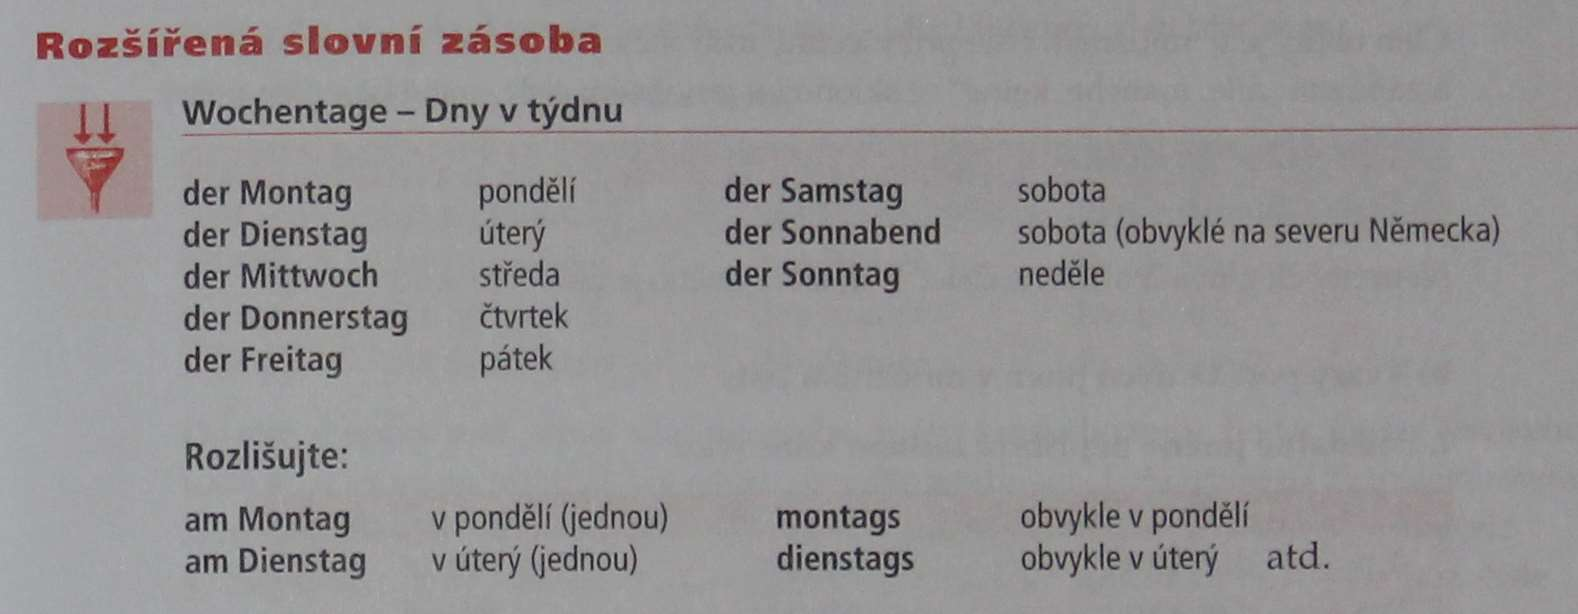
\includegraphics[width=1\linewidth]{L4_Wortschatz03.jpg}
      \caption*{ }
      \label{NJ:fig_L4_Wortschatz03}
    \end{figure}
    
    \subsection*{Skloňování podstatných jmen v množném čísle}
      \begin{itemize} % L4_Grammatik01.jpg
        \item \textbf{Skloňování určitého členu a některých zájmen v množném čísle:}
              \begin{table}[ht!]   % L4_Redensart01.jpg
                \hspace*{5em}
                \begin{tabular}{l|ll}
                  \hline
                  l.p. & die & meine, keine, alle, manche     \\
                  2.p. & der & meiner, keiner, aller, mancher \\
                  3.p. & den & meinen, keinen, allen, manchen \\
                  4.p. & die & meine, keine, alle, manche     \\
                  \hline
                \end{tabular}
                \caption*{ }
              \end{table}
              
              Člen určitý je v množném čísle pro všechny rody stejný. Všechna přivlastňovací 
              zájmena a zájmena „alle, manche, keine" se skloňují v množném čísle stejně jako člen 
              určitý.
              \begin{itemize}
                \addtolength{\itemindent}{5em}
                \item Haben Sie ein Kind?
                \item Haben Sie Kinder?
              \end{itemize}
              Neurčitý člen nemá množné číslo, podstatné jméno je pak bez členu.
        \item \textbf{Tvary podstatných jmen v množném čísle:}
          \begin{itemize}
            \item \textbf{Podstatné jméno nepřibírá žádnou koncovku}
              \begin{table}[ht!]   % L4_Grammatik02.jpg
                \hspace*{4em}
                \begin{tabular}{l|lll}
                       & \textbf{der Vater}  & \textbf{die Mutter}  & \textbf{das Rätsel}  \\
                  \hline
                  1.p. & die Vater           & die Mütter           & die Rätsel           \\
                  2.p. & der Väter           & der Mütter           & der Rätsel           \\
                  3.p. & den Vätern          & den Müttern          & den Rätseln          \\
                  4.p. & die Väter           & die Mütter           & die Rätsel           \\
                  \hline
                \end{tabular}
                \caption*{ }
              \end{table}
        
              Bez koncovky jsou především podstatná jména mužského a středního rodu, která končí v 
              jednotném čísle na \textbf{-er}, \textbf{-el}, \textbf{-en} a zdrobněliny, které jsou 
              vždy středního rodu a tvoří se příponami \textbf{-chen} a \textbf{-lein}. Z 
              podstatných jmen ženského rodu jsou bez koncovky jen dvě - \emph{„die Mutter"} a 
              \emph{„die Tochter"}. Některá podstatná jména této skupiny přehlasují (tzn. mění 
              kmenovou samohlásku: \emph{a - ä}, \emph{u - ü}, \emph{o - ö}, \emph{au - äu}).
      
            \item \textbf{Podstatné jméno přibírá v množné čísle koncovku -e}
              \begin{table}[ht!]   % L4_Grammatik02.jpg
                \hspace*{4em}
                \begin{tabular}{l|lll}
                       & \textbf{der Freund}   & \textbf{die Stadt}   & \textbf{das Jahr}    \\
                  \hline
                  1.p. & die Freunde           & die Städte           & die Jahre            \\
                  2.p. & der Freunde           & der Städte           & der Jahre            \\
                  3.p. & den Freunde\textbf{n} & den Städte\textbf{n} & den Jahre\textbf{n}  \\
                  4.p. & die Freunde           & die Städte           & die Jahre            \\
                  \hline
                \end{tabular}
                \caption*{ }
              \end{table}

              Tato skupina je zastoupena především u mužského rodu. V ženském rodě je zastoupena 
              pouze asi 40 podstatnými jmény, která přehlasují vždy, je-li v kmeni přehlasovatelná 
              samohláska. Podst. jména mužského a středního rodu přehlasují jen někdy.
              
            \item \textbf{Množné číslo má koncovku -er}
            \item \textbf{Množné číslo má koncovku -(e)n}
            \item \textbf{Množné číslo přebírá koncovku -s (pouze u některých cizích slov)}\newline
         \end{itemize}
      \end{itemize}
    
    \begin{figure}[ht!]
      \centering
      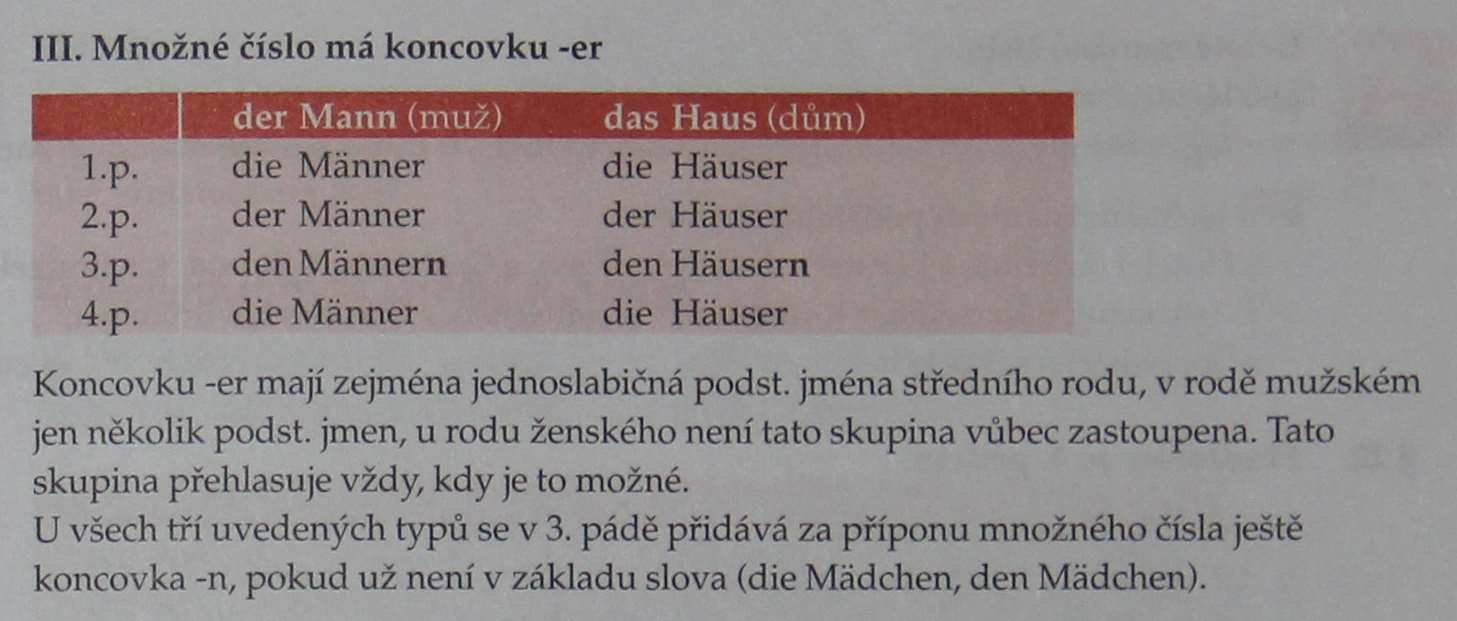
\includegraphics[width=1\linewidth]{L4_Grammatik03.jpg}
      \caption*{ }
      \label{NJ:fig_L4_Grammatik03}
    \end{figure}
    
    \begin{figure}[ht!]
      \centering
      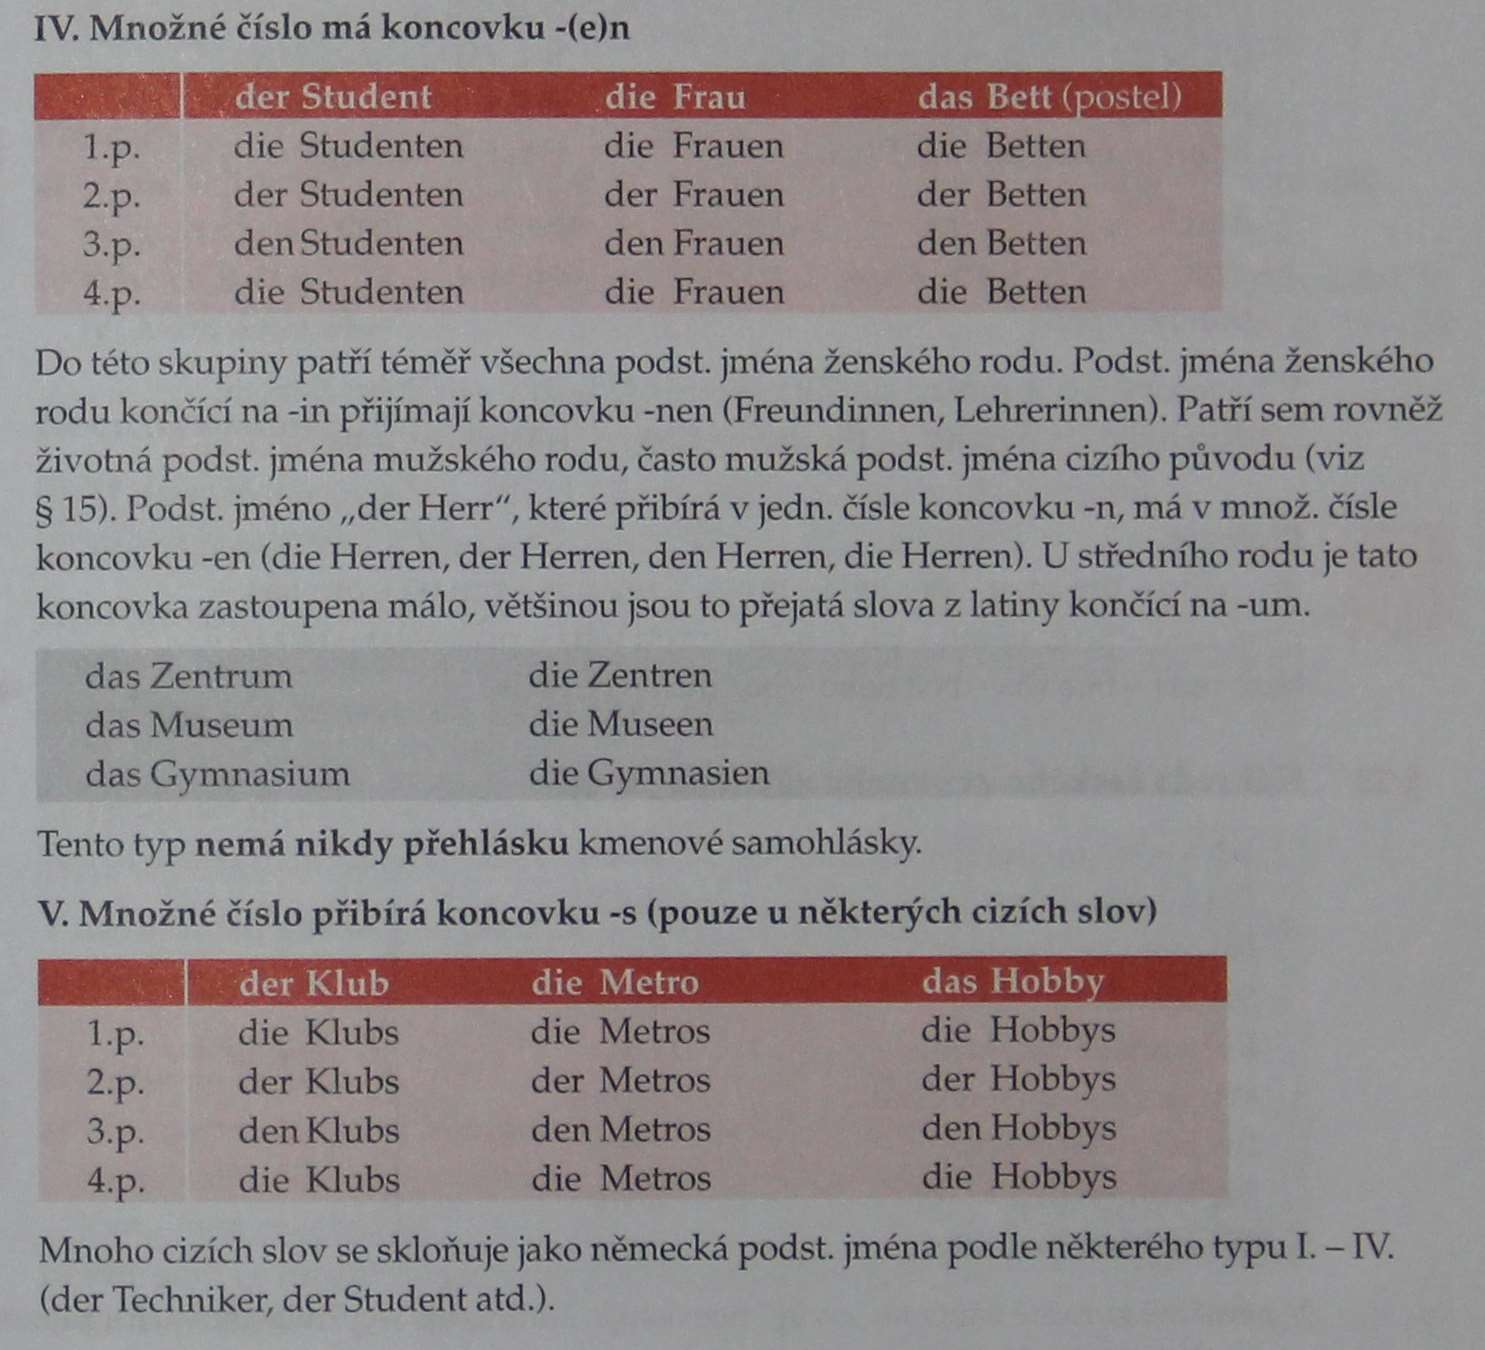
\includegraphics[width=1\linewidth]{L4_Grammatik04.jpg}
      \caption*{ }
      \label{NJ:fig_L4_Grammatik04}
    \end{figure}
    
    \begin{figure}[ht!]
      \centering
      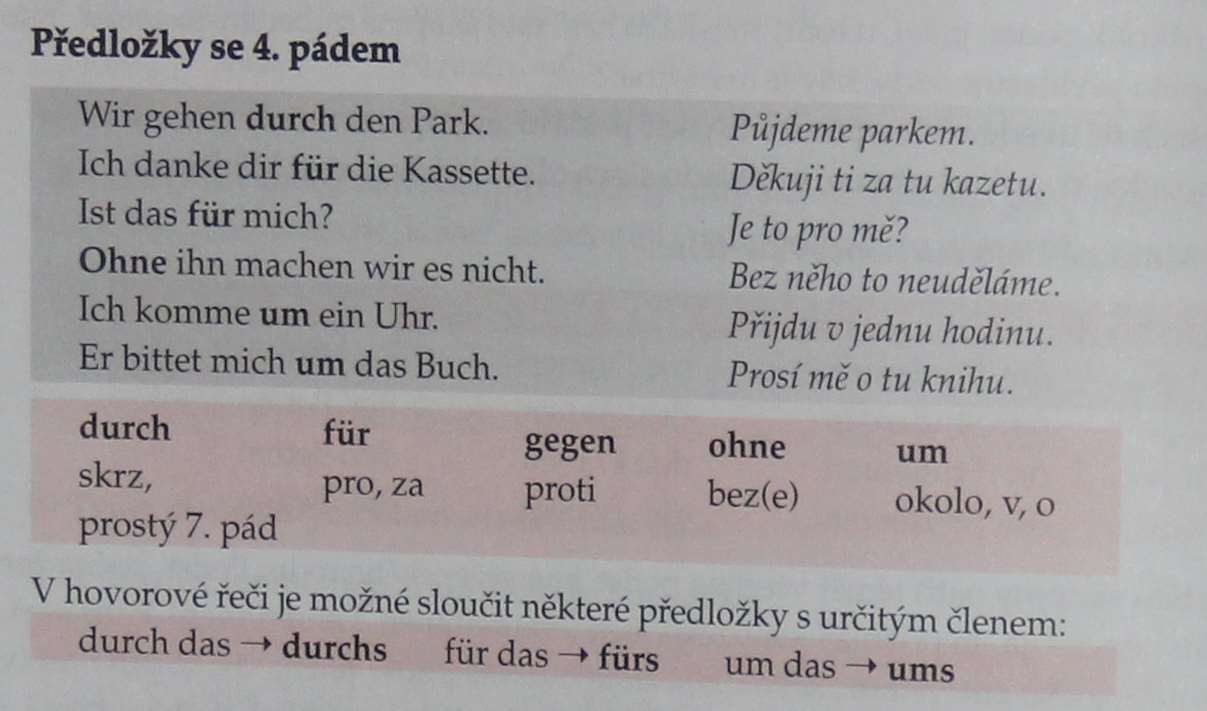
\includegraphics[width=1\linewidth]{L4_Grammatik05.jpg}
      \caption*{ }
      \label{NJ:fig_L4_Grammatik05}
    \end{figure}
    
    \begin{figure}[ht!]
      \centering
      
\includegraphics[width=1\linewidth]{L4_Grammatik06.jpg}
      \caption*{ }
      \label{NJ:fig_L4_Grammatik06}
    \end{figure}
    
    \begin{figure}[ht!]
      \centering
      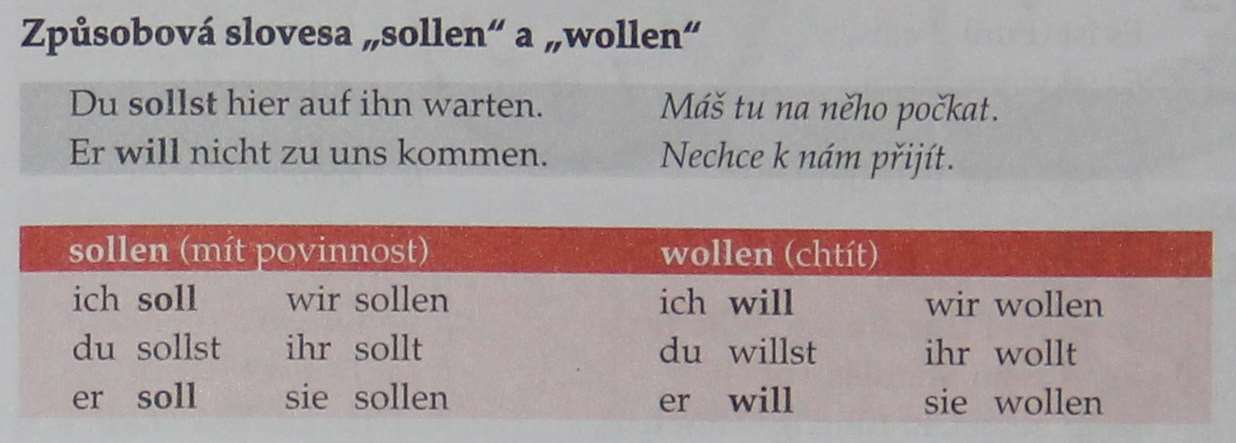
\includegraphics[width=1\linewidth]{L4_Grammatik07.jpg}
      \caption*{ }
      \label{NJ:fig_L4_Grammatik07}
    \end{figure}
    
    \begin{figure}[ht!]
      \centering
      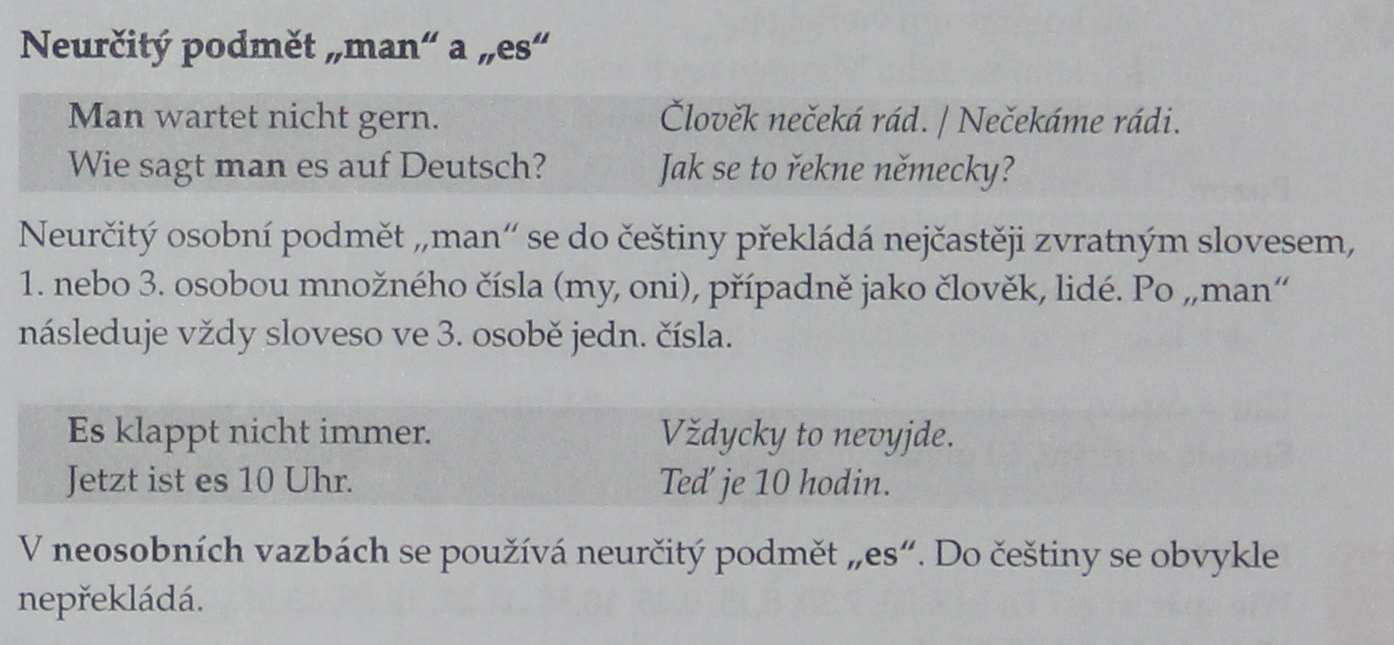
\includegraphics[width=1\linewidth]{L4_Grammatik08.jpg}
      \caption*{ }
      \label{NJ:fig_L4_Grammatik08}
    \end{figure}
  % !TeX spellcheck = de_DE
%================ Kapitola 5: Guten Appetit! =======================================================
\setchaptertoc
\chapter{Lektion 5: Guten Appetit!}\label{NJ:chap_N1_L5}
  
  \section*{Slovní zásoba}

      



















































  % !TeX spellcheck = de_DE
%================ Kapitola 6: Karin und Horst ziehen um ============================================
\chapter{Lektion 6: Karin und Horst ziehen um}\label{NJ:chap_N1_L6}
\minitoc
  
  \section{Slovní zásoba}
    \begin{table}[ht!]   % L4_Wortschatz01.jpg
      \centering
      \begin{tabular}{llll}
        \hline
          der, die, das erste     & první    & r, e, s nächste        & příští, další, nejbližší  \\
          eigen                   & vlastní  & e Prüfung, -, en (in)  &  zkouška (z)              \\
          aussehen, du siehst aus & vypadat  &  ablegen, du legst ab  & složit (zkoušku)          \\
          r Flur, (e)s, e         & předsíň  & e Geduld, -, 0         & trpělivost                \\
          e Tür, -, en            & dveře    & weil                   & protože                   \\
          führen                  & vést     & jeder, jede, jedes     & každý, každá, každé       \\
          schlafen, du schläfst   & spát     &  lieber                & raději                    \\
          s Schlafzimmer, s, -    & ložnice  & eng                    & úzký, úzce, těsný, -ě     \\
          e Küche, -, n           & kuchyně  & e Anbaumöbel (mn.č.)   & sektorový (stavebnicový)  \\
          s Bad, (e)s, ä-er       & koupelna &                        &  nábytek                  \\
          eingerichtet            & zařízený &  r Stuhl, (e)s, ü-e    & židle                     \\
          s Bett, es, en          & postel   & sitzen                 &  sedět                    \\
          s Kleid, (e)s, er       & šaty (dámské) & nachdenken, du    & přemýšlet (o)             \\
          r Schrank, (e)s, ä-e    & skříň         & denkst nach       &                           \\
          hell                    & světlý, -e    &  (über 4.p.)      &                           \\
          e Möbel (mn.c.)         & nábytek       & s Studenten(wohn)-& kolej                     \\
          an (3./4.p.)            & na (svislé ploše), u, k   & heim, (e)s, e  &                  \\
          recht                   & pravý         & lieb              & milý, -e                  \\
          e Wand, -, ä-e          & stěna         & vielmals          & mnohokrát                 \\
          stehen                  & stát          &  r Brief, (e)s, e & dopis                     \\
          r Fernseher, s, -       & televizor     & wissen, ich weiß  & vědět                     \\
          bequem                  & pohodlný, -ě  & billig            & levný, -ě, laciný, -ě     \\
          neben (3./4.p.)         & vedle         & bezahlen          & (za)platit                \\
          e Sitzgarnitur, -, en   & sedací souprava  & e Miete, -, n  & nájemné                   \\
          zwischen (3./4.p.)      & mezi (dvěma)  & pro               &  za, pro, na              \\
          s Sofa, s, s            & pohovka       & r Stock, (e)s, Stock-  & poschodí             \\
          r Sessel, s, -          & křeslo        & werke             &                           \\
          r Couchtisch,(e)s.      & konferenční stolek  & modern      & moderní                   \\
          e [kauč-]               &               & zusammen          & společně, dohromady       \\
          unter (3./4.p.)         & pod, mezi (více) & s Studienjahr, (e)s, e  & ročník (studia)  \\
          s Fenster, s, -         & okno          & e Fachrichtung, -, en      & obor, zaměření   \\
          e Blume, -, n           & květina       & helfen, du hilfst & pomáhat, pomoci           \\
          e Ecke, -, n            & roh, kout     & r Briefumschlag,  & obálka                    \\
          verschieden             & různý, -ě     & (e)s, ä-e         &                           \\
          s Heft, (e)s, e         & sešit         &  ergänzen         & doplnit, -ňovat           \\
          e Zeitung, -, en        & noviny        & geboren           & narozen(ý)                \\
          e Zeitschrift, -, en    & časopis       &                   &              \\
         \hline
      \end{tabular}
      \caption*{}
    \end{table}
      



















































} % DEBUG was off

}
{
% DEBUG was off
    %     Železniční zabezpečovací technika
% notes:
%~~~~~~~~~
% notes:
%~~~~~~~~~
% \label{zzt:eq000}
% \label{zzt:fig001}
% \label{zzt:exam000}
% \label{zzt:tab000}
%---------------------------------------------------------------------------------------------------
% Setting path to image 
\graphicspath{{../src/ZZT/img/}}
%---------------------------------------------------------------------------------------------------
% file ZZT.tex
%--------------------------------------------------------------------------------------------------
\setpartpreamble[u]{
  \begin{center}
    \vspace{1cm}
    \Huge \uppercase{\textbf{Bezpečnost v}} \\
    \Huge \uppercase{\textbf{železniční dopravě}} \\
    \vspace{2cm}
    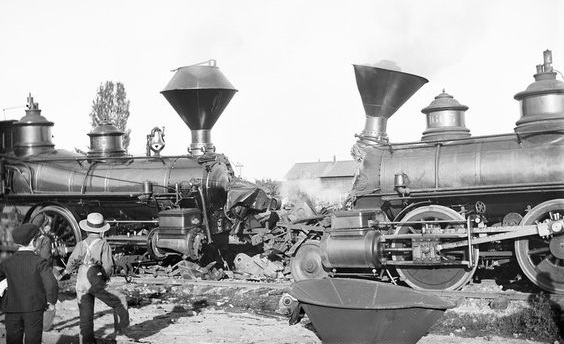
\includegraphics[width=0.8\linewidth]{BZT.jpg}
  \end{center}
}

\part{BZT}\label{part:BZT}
\parttoc

\ifthenelse{ \equal{\DebugMode}{true} }{
% Debug mode ON
  % !TeX spellcheck = cs_CZ
%{\tikzset{external/prefix={tikz/PZT/}}
% \tikzset{external/figure name/.add={ch02_}{}}
%---------------------------------------------------------------------------------------------------
% file ra3ch001.tex
%---------------------------------------------------------------------------------------------------
%======================== Kapitola: Železniční zabezpečovací technika ============================
%\begin{Czech}
\chapter{Obsah zabezpečovací techniky}\label{bzt:chapI}
\minitoc
  Důležitým odvětvím v železniční dopravě je odvětví zabezpečovací techniky. Potřeba zabezpečení 
  železničního provozu vznikala již v prvních začátcích železniční dopravy, ale postupný rozvoj 
  železniční dopravy si vynutil stále větší požadavky na konstrukci nových druhů zařízení a na 
  odbornost pracovníků pro jejich obsluhu.
  
  Tyto příručka je určena jako studijní materiál nezbytný pro implementaci moderních 
  metod návrhu zabezpečovacích systémů v železniční dopravě. 
   
\section{Náplň zabezpečovací techniky}
  Klasická železniční zabezpečovací zařízení jsou definována jako zařízení, která prvořadě 
  kontrolují, zda zamýšlené disposice dopravních zaměstnanců jsou bezpečné a zda jím nařízené 
  výkony se provádějí tak, aby nebyla ohrožena bezpečnost železniční dopravy. Pro přiblížení 
  uvažujme část stanice podle obr. \ref{zzt:fig001} a na této situaci s určitými zjednodušeními 
  tento obsah naznačme.

  \begin{figure}[ht!] %\ref{zzt:fig001}
    \centering
    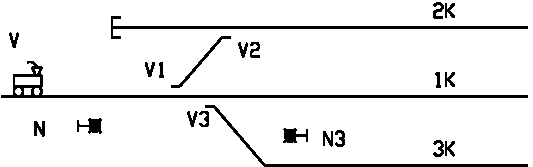
\includegraphics[width=0.8\linewidth]{zzt_fig001.pdf}
    \caption{Stanice
             (\cite[s.~5]{Chudacek2005})}
    \label{zzt:fig001}
  \end{figure}
 
  Před stanicí je umístěno návěstidlo \(N\), které v základní poloze ukazuje návěst \uv{stůj}. Dokud
  návěstidlo ukazuje tuto návěst, nesmí vlak \(V\) do stanice vjet. Má-li vlak vjet bezpečně např. 
  na kolej \(1K\), je třeba splnit určité podmínky. Výměny - pohyblivé části výhybek - \(V1\) a 
  \(V3\) musí být v poloze umožňující řádnou jízdu na kolej \(1K\), tj. jeden jazyk musí
  vždy přiléhat k příslušné opornici, druhý musí být od své opornice náležitě vzdálen. Na koleji 
  \(1K\) (včetně výhybek \(V1\) a \(V3\)) nesmí být žádná vozidla a ani nesmí být povolen příjezd
  jiných vozidel na tuto kolej z opačného směru. Zamýšlenou cestu nesmí ohrožovat z boku pohyby 
  jiných vlaků nebo posunujících dílů, proto výměna \(V2\) musí kolizní jízdu svou polohou 
  znemožňovat a návěstidlo \(N3\) musí kolizní jízdu zakazovat (ochrana odvratnou polohou výměny se 
  nazývá \emph{přímou boční ochranou}, ochrana návěstidlem se zakazující návěstí je \emph{nepřímou 
  boční ochranou}). Když tedy byly všechny prvky zvolené cesty správně nastaveny, přezkoušeny a 
  shledány bez závady, může být návěstidlo \(N\) přestaveno do polohy dovolující jízdu. Po celou 
  dobu, kdy návěstidlo dovoluje jízdu, bude dohlíženo, že všechny k tomu rozhodující podmínky jsou 
  nadále splněny. Vlak \(V\) vjede do stanice a ihned po jeho vjezdu se návěstidlo \(N\) přestaví 
  opět do základní polohy (návěst "stůj"), aby týž povel návěstidla nemohl být využit více vlaky a 
  aby shora uvedený postup bylo třeba pro každý vlak znovu opakovat.

  \begin{figure}[ht!] %\ref{zzt:fig002}
    \centering
    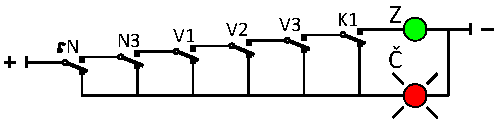
\includegraphics[width=0.8\linewidth]{zzt_fig002.pdf}
    \caption{Vybavení koleje technickým zařízením, které dohlíží na aby vlak vjel do stanice 
             bezpečně
             (\cite[s.~5]{Chudacek2005})}
    \label{zzt:fig002}
  \end{figure}
  
  Úkony, potřebné k tomu, aby vlak vjel do stanice bezpečně, může vykonat určený zaměstnanec. Ten
  se například pochůzkou přesvědčí, že kolej \(1K\) je volná, že výměny jsou řádně postaveny atd. a 
  po ověření všech podmínek přestaví návěstidlo \(N\) do polohy povolující jízdu. Pokud se 
  zaměstnanec nezmýlí, nedojde k nehodě (povšimněme si, že negace této věty nemusí být pravdivá). 
  Bezpečnost jízdy vlaku bude tedy závislá na osobních vlastnostech člověka. Aby tomu tak nebylo, 
  vybavíme koleje technickým zařízením, které bude na jejich volnost dohlížet, výměny jinými
  technickými zařízeními, která budou kontrolovat jejich polohu atd. a jízdní návěst návěstidel
  učiníme nuceně závislou na informacích těchto technických zařízení. Primitivní schéma
  takového zařízení je na obr. \ref{zzt:fig002}. I když pak dopravní zaměstnanec dá návěstním 
  řadičem \(N\) pokyn k rozsvícení jízdní (tj. jízdu povolující) návěsti \(Z\), návěst se rozsvítí 
  jen v případě, že kontakt \(N3\) informuje svým sepnutím, že návěstidlo \(N3\) skutečně ukazuje 
  návěst "stůj", kontakty \(V1\), \(V2\) a \(V3\) informují, že výměny jsou ve správné poloze a 
  kontakt \(K1\) informuje, že první kolej je volná a není na ni postavena jiná cesta. Jízdní 
  návěst \(Z\) se tedy rozsvítí až po splnění všech předem stanovených podmínek pro bezpečný vjezd 
  vlaku. Není-li kterákoliv podmínka splněna, na návěstidle \(N\) zůstává svítit červené světlo Č. 
  
  Přesto takové zařízení \textbf{nelze} považovat za zabezpečovací zařízení. Prvním důvodem je, že 
  nebyly zřízeny \emph{vzájemné závislosti}. Jízdní návěst na návěstidle \(N\) se sice rozsvítí až 
  když jsou splněny všechny podmínky, ale výměny a návěstidla zůstala volná. Nic nebrání, aby se 
  např. poloha výměn změnila dříve, než vlak \(V\) ukončí svou jízdu. Zhasnutí jízdního znaku \(Z\) 
  na návěstidle \(N\) v důsledku ztráty kontroly při přestavení výměny už nemusí být nic platné, 
  protože vlak již mohl návěstidlo minout nebo již není schopen včas zastavit. Nepostačí ale ani 
  zřízení vzájemné závislosti tím, že by rozsvícená jízdní návěst \(Z\) uzavírala výměny a 
  návěstidla v žádoucí poloze (např. prostřednictvím sériově řazeného relé). Vzhledem k nebezpečí
  přerušení sekvence postupných kroků je důležité, aby uzavření výměn a návěstidel bylo provedeno 
  dříve, než se rozsvítí jízdní návěst. Postup stavění jízdní cesty, vyhovující požadavkům 
  zabezpečovací techniky, bude tedy v naznačeném příkladě následující:
  \begin{itemize}\addtolength{\itemsep}{-0.5\baselineskip}
    \item nejprve se přestaví výměny do žádané polohy,
    \item v druhém úkonu (nazývaném závěr jízdní cesty) se při uzavírání výměn a návěstidel 
          přezkouší jejich správná poloha a tedy, že první úkon byl řádně proveden. Pokud první 
          úkon nebyl proveden správně, musí být znemožněn úkon druhý,
    \item obdobně třetí úkon, tj. rozsvícení jízdní návěsti na návěstidle \(N\), je možný jen 
          tehdy, byl-li druhý úkon (a tedy i první úkon) řádně proveden. 
  \end{itemize}
  
  Tím jsme dosáhli požadované \emph{vzájemné závislosti}, jejíž popsaná úroveň je \textbf{prvním
  charakteristickým rysem} zabezpečovacího zařízení. Zařízení z obr. \ref{zzt:fig002} bude podmínce 
  vyhovovat například v případě, že návěstní přepínač \(N\) bude konstrukčně upraven tak, že ho 
  nebude možné přeložit bez provedení \textbf{závěru jízdní cesty}. Důsledkem zavedení závěru 
  jízdní cesty bude potřeba po vlaku jízdní cestu vybavit, tj. závěr zrušit, aby bylo možné s 
  jednotlivými prvky opět volně manipulovat. 

  Ani nyní však ještě nelze v uvedeném příkladě hovořit o zabezpečovacím zařízení. Zařízení musí
  být konstruováno tak, aby \emph{bezpečnost byla zachována i při jakékoliv možné poruše vlastního 
  zařízení}. Tento  požadavek platí jak pro jednotlivé části, tak pro celek a je \textbf{druhým 
  charakteristickým rysem} železniční zabezpečovací techniky. V uvedeném případě to znamená, že 
  zařízení pro kontrolu volnosti koleje nesmí ani při poruše hlásit obsazenou kolej jako volnou, 
  zařízení pro kontrolu polohy výměny nesmí ani při poruše hlásit nesprávně postavenou výměnu jako 
  výměnu správně postavenou, ke zrušení závěru jízdní cesty nesmí ani poruchou dojít dříve než vlak 
  dotčené prvky skutečně mine atd. Právě tak vlastní zapojení pro rozsvícení jízdní návěsti musí 
  být konstruováno tak, aby se jízdní návěst nemohla poruchou zapojení rozsvítit, pokud všechny 
  podmínky pro její svícení nebudou splněny. Jak patrno, vychází se ze základního železničního
  bezpečnostního předpokladu, že zastavení vlaku poskytuje nejvyšší bezpečnost. Tento předpoklad se 
  zásadně liší od principů aplikovaných v letecké dopravě, kosmonautice, nukleární technice, 
  navigaci, řízení procesů, robotice, dolování, systémech zabezpečení proti vloupání či odcizení 
  atd., kde je prozatím obvykle hlavním cílem dosažení maximální spolehlivosti a pohotovosti 
  systému.
  
  Důsledkem druhého charakteristického rysu zabezpečovací techniky, tj. převedení všech poruch
  bezpečnějším směrem je, že téměř každá porucha zabezpečovacího zařízení znamená omezení dopravy. 
  To samozřejmě může vést k narušení plynulosti a vzniku provozních nepravidelností, což jsou jevy, 
  které samy o sobě nebezpečí v dopravě výrazně zvětšují. Ve vážnějších případech je nutné 
  zabezpečovací zařízení do skončení jeho opravy zcela vypnout, aby byl možný alespoň omezený pohyb 
  vlaků. Pak se ovšem provoz, jehož pravidelnost je navíc narušena, děje bez jakékoliv podpory 
  zabezpečovacího zařízení, zatížen, byť i jen na omezenou dobu, možnými lidskými omyly. Odtud tedy 
  plyne třetí charakteristický rys zabezpečovací techniky, což je taková konstrukce zařízení, která 
  má co nejméně poruch, tedy vysokou spolehlivost nebo - obecněji - co nejvyšší pohotovost. 
 
  Úloha zabezpečovací techniky nekončí zajištěním odpovídajícího návěstního znaku na návěstidle.
  Také na lokomotivě je strojvedoucí, jemuž je svěřena péče o bezpečnost vlaku a který tuto 
  bezpečnost může ohrozit svým omylem. Působnost zabezpečovacích zařízení se tedy (prostřednictvím 
  vlakového zabezpečovacího zařízení) prodlužuje až na vozidlo, aby se zajistilo, že vlak také 
  skutečně bude návěsti respektovat. 

  Aplikují-li se všechny výše uvedené zvláštnosti správně při vývoji zabezpečovacího systému, je
  třeba se postarat také o to, aby nedošlo k jejich znehodnocení při projekci, výrobě, montáži a 
  údržbě konkrétních zařízení. Při těchto činnostech je také třeba počítat s lidskými vlastnostmi. 
  Zařízení, sloužící primárně pro eliminaci chyb dopravních zaměstnanců konstruují, vyrábějí, 
  montují a udržují opět lidé. Naštěstí tyto práce, na rozdíl od výkonu dopravní služby, probíhají 
  (nebo by rozhodně měly probíhat) v lepších podmínkách a bez časové tísně. Za příznivých podmínek 
  se nedokonalosti člověka tolik neuplatňují a práci každého pracovníka lze kontrolovat jinými s 
  případnou pomocí dalších technických zařízení. Přesto však z toho pro projekci, výrobu, montáž a 
  údržbu zabezpečovacích zařízení vyplývají jisté zvláštnosti. 
  
  Vedle úloh z oblasti bezpečnosti plní moderní zabezpečovací technika i úkoly další. Především jde
  o hlubší zásahy do vlastního provozu prostředky automatizace. Ta pak, při správném provedení, 
  vede k zlepšenému využití technických prostředků železnic (např. zvýšení propustné výkonnosti 
  tratí), k zhospodárnění provozu, k úspoře jiných, podstatně vyšších investičních nákladů (např. 
  budování další koleje). Protože však zabezpečovací zařízení je zařízením v zásadě restriktivním, 
  nelze u něj bezhlavě prosazovat zvyšování výkonnosti vždy a ve všech směrech. Později také 
  uvidíme, že zabezpečovací technika se podílí na zvyšování bezpečnosti i v jiných oblastech: 
  kolejové obvody alespoň částečně dohlíží na stav jízdní dráhy (celistvost kolejnic), přestavná 
  zařízení výměn dohlíží na stav výhybek, vlakové zabezpečovače mohou do určité míry dohlížet na 
  stav brzdové soustavy vlaku (sledováním skutečně dosaženého odrychlení při brzdění), přejezdová 
  zabezpečovací zařízení se podílejí na eliminaci cizích vlivů na dopravu atd.
  
  Souhrnně lze konstatovat, že prvořadým účelem zabezpečovacích zařízení na železnici je
  předcházet kolizím a vykolejení vlaků z důvodu chybného řízení dopravy. K tomu účelu je u 
  zařízení třeba sledovat následující oblasti:
  \begin{itemize}\addtolength{\itemsep}{-0.5\baselineskip}
    \item funkční bezpečnost (korektnost systému), tj. řádné plnění všech požadovaných funkcí v 
          bezporuchovém stavu a při očekávaných vlivech pracovního prostředí,
    \item technickou bezpečnost (bezpečnou konstrukci), tj. splnění požadavku, aby nedošlo k 
          přímému ohrožení bezpečnosti dopravy ani při poruchách samotného zabezpečovacího zařízení,
    \item bezpečnou aplikaci, tj. vytvoření takových logických funkcí a vzájemných závislostí, aby 
          pro konkrétní situaci navržené zařízení ve všech provozních stavech mohlo řádně plnit 
          svou funkci (na jeho výstupech budou jízdu povolující informace pouze v takovém rozsahu, 
          který odpovídá stavu informací vstupních) a zajištění, aby tyto vlastnosti zařízení mělo 
          i po výrobě a montáži,
    \item bezpečný provoz a údržbu, tj. zajištění, že předchozí úrovně zůstanou v zařízení 
          zachovány po celou dobu životnosti,
    \item vysokou spolehlivost, tj. omezení případů, kdy nepřímo, vyřazením zabezpečovacího 
          zařízení a přechodem na manuální řízení, by mohlo dojít k ohrožení bezpečnosti dopravy.
  \end{itemize}
  Žádnou ze zmíněných oblastí nelze preferovat, protože žádná nemůže nahradit druhou a             
  nedostatky v kterékoliv z nich znehodnocují výsledky ostatních.
  
  Přímým obsahem železniční zabezpečovací techniky není zajištění zdraví a bezpečnosti
  zaměstnanců (i když provozovaná zařízení samozřejmě musí splňovat i požadavky např. ve směru 
  ochrany před nebezpečným dotykovým napětím, ergonomicky správně navrženého obsluhovací pracoviště 
  atd.), zabránit nehodám ze zlého úmyslu, násilnou obsluhou, úmyslným poškozením nebo zneužitím 
  zařízení. V poslední době se však jeví jako nezbytné dokonaleji zajišťovat zabezpečovací zařízení 
  proti vandalům a lapkům všeho druhu a neoprávněným zásahům do zařízení v případě, že používají 
  jiných než speciálně drážních zařízení (viz dále např. ochrana dat v otevřených sítích).  

\section{Třídění}
  K železničním zabezpečovacím zařízením se obvykle řadí i zabezpečovací zařízení používaná na
  podzemních drahách (metro, doly), na pouličních drahách (tramvaje - zejména městské rychlodráhy) 
  a na vlečkách, protože využívají obdobných principů, často i obdobná nebo jen poněkud upravená 
  zařízení. Při třídění zařízení lze použít řadu třídících hledisek; téměř vždy se však vyskytnou 
  zařízení přechodová (smíšená) nebo podle užitého třídění obtížně definovatelná. Přesto je dále 
  několik třídění uvedeno, protože poskytují obrázek o pestrosti a mnohotvárnosti pojednávaného 
  zařízení. 
  
  Nejpřirozenějším a klasickým tříděním zabezpečovacích zařízení je třídění podle účelu zařízení.
  Podle tohoto hlediska lze zabezpečovací zařízení dělit na zařízení: 
  \begin{itemize}\addtolength{\itemsep}{-0.5\baselineskip}
    \item staniční,
    \item traťové,
    \item vlakové,
    \item přejezdové, 
    \item spádovištní. 
  \end{itemize}
  Účel je patrný již z názvu. Staniční zabezpečovací zařízení zajišťuje bezpečný pohyb vlaků ve 
  stanici, traťové zařízení zabezpečuje jízdu vlaku na trati mezi stanicemi, vlakové zařízení 
  zabraňuje vlaku pohybovat se nad rámec, který povoluje zařízení staniční a traťové (s případným 
  zahrnutím i dalších omezení), přejezdové zařízení přispívá k zajištění bezpečnosti na úrovňovém 
  křížení silnice a železnice informováním uživatelů silnice, že se k přejezdu blíží vlak s 
  předností v jízdě. Nad všemi těmito zařízeními pak může být budováno zařízení pro dálkové 
  ovládání většího úseku tratě z jednoho místa. 
  
  Podle místa ovládání zařízení mluvíme o zařízení s obsluhou :
    \begin{itemize}\addtolength{\itemsep}{-0.5\baselineskip}
    \item místní,
    \item ústřední (centralizovanou v oblasti jedné stanice),
    \item dálkovou (mimo vlastní stanici).
  \end{itemize}

  Další třídění je odvozeno od způsobu ovládání periferií (výměn, návěstidel atd.) a tak vlastně
  zahrnuje celou historii železniční zabezpečovací techniky. Rozeznáváme zařízení:
  \begin{itemize}\addtolength{\itemsep}{-0.5\baselineskip}
    \item mechanická (využívající výhradně lidské síly),
    \item elektrická,
    \item pneumatická,
    \item hydraulická. 
  \end{itemize}

  Obdobně, v následujícím třídění je rozhodující způsob, jímž se v zařízení potřebné závislosti
  realizují. Zde rozeznáváme zařízení se závislostmi:
  \begin{itemize}\addtolength{\itemsep}{-0.5\baselineskip}
    \item mechanickými,
    \item mechanickými i elektrickými (tzv. elektromechanická a elektrodynamická zařízení),
    \item elektrickými, která lze dále dělit podle rozhodujících stavebních prvků, jimiž jsou 
         závislosti realizovány, na zařízení:
       \begin{itemize}
       \item reléová,
       \item hybridní (rozhodující část bezpečné logiky je realizována reléově, zbytek 
             elektronicky),
       \item elektronická (mikroprocesorová). 
       \end{itemize}
  \end{itemize}

  U traťových zabezpečovacích zařízení je kladen důraz na rozsah spolupůsobení vlaku. Zařízení se
  pak dělí na:
  \begin{itemize}\addtolength{\itemsep}{-0.5\baselineskip}
    \item poloautomatická (poloautobloky),
    \item automatická (autobloky).
  \end{itemize}
  Podle rozmístění traťových zařízení podél trati lze automatická zařízení dále dělit na:
  \begin{itemize}\addtolength{\itemsep}{-0.5\baselineskip}
    \item decentralizovaná (funkční bloky jsou umístěny v každém návěstním bodě),
    \item částečně centralizovaná (funkční bloky jsou umístěny pouze ve vybraných bodech na trati),
    \item centralizovaná (zařízení je koncentrováno do stanic).
  \end{itemize}
  Vlaková zabezpečovací zařízení se dělí podle způsobu přenosu informací mezi tratí a hnacím
  vozidlem na zařízení:
  \begin{itemize}\addtolength{\itemsep}{-0.5\baselineskip}
    \item bodová,
    \item semiliniová,
    \item liniová. 
  \end{itemize}

  Podle způsobu kontroly souladu jízdy vlaku s přenášenými informacemi se vlaková zařízení dále 
  dělí na zařízení s kontrolou:
  \begin{itemize}\addtolength{\itemsep}{-0.5\baselineskip}
    \item bdělosti strojvedoucího,
    \item rychlosti vlaku.
  \end{itemize}
  
  Zařízení přejezdová se dělí podle způsobu výstrahy na přejezdová zařízení:
  \begin{itemize}\addtolength{\itemsep}{-0.5\baselineskip}
    \item mechanická,
    \item světelná bez závor,
    \item světelná se závorami.
  \end{itemize}
  
  U moderních systémů dělení zabezpečovacích zařízení na zařízení staniční, traťová, vlaková a
  přejezdová ztrácí smysl, protože systémy jsou komplexní, se společným jádrem řídícím jednotlivé 
  periférie a tyto celky pak tvoří nanejvýš podsystémy. Na obr. 3-1 je základní blokové schéma 
  takového systému. 
  \begin{figure}[ht!] %\ref{zzt:fig003}
    \centering
    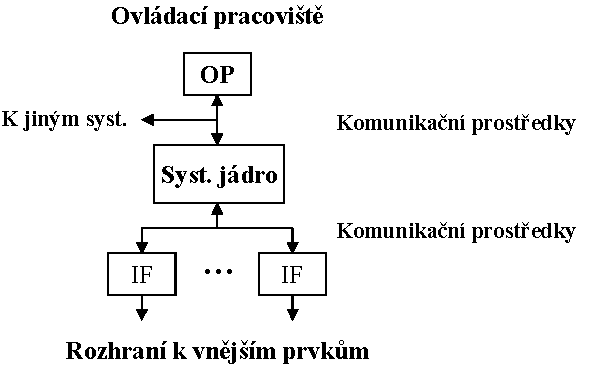
\includegraphics[width=0.8\linewidth]{zzt_fig003.pdf}
    \caption{Stanice
             (\cite[s.~11]{Chudacek2005})}
    \label{zzt:fig003}
  \end{figure}


  \section{Klasifikace poruch}
    \textbf{Chyba} je rozdíl mezi správnou a skutečnou hodnotou nějaké veličiny. V zařízení se 
    chyby mohou obecně objevit jako \emph{důsledek (projev) poruchy některé jeho součásti, 
    působením nějakého cizího vlivu} nebo \emph{selháním lidského činitele}. Za poruchy hardware se 
    považují všechna vybočení z předpokládaných vlastností stavebního prvku (součástky, dílu) 
    zařízení. Předpokládanými vlastnostmi prvků přitom jsou vlastnosti odpovídající příslušným 
    technickým podmínkám popisujícím jeho vlastnosti. Jako omyl lze označit každou lidskou činnost, 
    která může vést k nezamýšlenému chování zařízení. V širším slova smyslu se jako 
    \textbf{porucha} označují souhrnně všechny příčiny vedoucí k chybě, tj. poruch součásti, 
    cizí vliv i omyl.

%~~~~~~~~~~~~~~~~~~~~~~~~~~~~~~~~~~~~~~~~~~~~~~~~~~~~~~~~~~~~~~~~~~~~~~~~~~~~~~~~~~~~~~~~~~~~~~~~~~
\printbibliography[title={Seznam literatury}, heading=subbibliography]
\addcontentsline{toc}{section}{Seznam literatury}

\chapter{Bezpečnost a spolehlivost zabezpečovacích systémů}
 \section{Spolehlivost}
 \section{Bezpečnost}
    V různých publikacích je možné najít různé definice bezpečnosti. Například norma 
    EN~61508\footnote{Funkční bezpečnost elektrických/elektronických/programovatelných 
    elektronických systémů souvisejících s bezpečností (Functional safety of electrical/ 
    electronic/programmable electronic systems), obecná norma funkční bezpečnosti, která se opírá o 
    dvě základní koncepce - životní cyklus bezpečnosti a úroveň integrity bezpečnosti 
    (\texttt{SIL})} 
    definuje bezpečnost jako nepřítomnost netolerovaného rizika. Z této definice je zřejmé, že 
    bezpečnost je úzce spjatá s rizikem, a je nutné bezpečnost třeba chápat relativně. Když se 
    řekne, že řídicí systém je bezpečný, neznamená to jeho absolutní bezpečnost (ta je prakticky 
    nedosažitelná vzhledem na existenci objektivních faktorů, jako je například úroveň poznání, 
    technologická úroveň a limitované finanční prostředky), ale taková úroveň bezpečnosti, 
    která zodpovídá definovaným bezpečnostním požadavkům na tento řídicí systém. 

    Relativnost v pojímání bezpečnosti znamená posun od kvalitativního ke kvantitativnímu chápaní bezpečnosti.

    Kvalitativně je bezpečnost chápána jako schopnost řídicího systému zajistit omezení důsledků 
    poruch řídicích systému v daných podmínkách a v daném časovém intervalu. Matematicky je možné 
    kvalitativní bezpečnost řídicího systému vyjádřit jako 
    \begin{equation}
      E_H = 0,
    \end{equation}
    kde \(E_H\) je množina nebezpečných stavů, které jsou důsledkem výskytu pravděpodobných poruch 
    řídicího systému. Pravděpodobná porucha je taková porucha z množiny všech poruch, jejichž 
    výskyt během provozu řídicího systému je nutné předpokládat (vzhledem na požadovanou úroveň 
    bezpečnosti řídicího systému).
	
    Kvantitativně je bezpečnost řídicího systému chápána jako pravděpodobnost nepřítomnosti
    jakéhokoliv nebezpečného stavu v řídicím systému v daných podmínkách a v daném časovém
    intervalu. Je zřejmé, že i když pravděpodobnost nebezpečného stavu řídicího je malá, neznamená
    to, že se nebezpečný stav nemůže vyskytnou v nejbližším časovém intervalu, Matematicky je možné
    kvantitativní bezpečnost vyjádřit tak, že
    \begin{equation}
      P_{HT}(t)\geq P_{HT}(t)>0,
    \end{equation}
    kde \(P_{HT}(t)\) je pravděpodobnost tolerovaného nebezpeční řídicího systému a \(P_{HR}(t)\)
    je reálná pravděpodobnost nebezpeč\-ného stavu řídicího systému.
	 
    Na kvantitativním hodnocení bezpečnosti řídicího systému je v podstatě možné uplatnit stejné 
    teoretické postupy, jako při hodnocení spolehlivosti technických systémů. Zásadní rozdíl je v 
    tom, že při hodnocení spolehlivosti standardních řídicích systémů se obvykle rozlišují dva 
    stavy - bezporuchový stav a poruchový stav, a k těmto dvěma stavům se vztahují také 
    kvantitativní ukazatele spolehlivosti. Při hodnocení bezpečnosti řídicích systémů musíme 
    uvažovat s dvěma druhy poruchových stavů - bezpečným a nebezpečným poruchovým stavem. 
    Bezpečnost řídicího systému se potom vyjadřuje pomocí ukazatelů bezpečnosti (například 
    pravděpodobnost výskytu nebezpečné poruchy, intenzita nebezpečných poruch, ...).

    Při kvantitativním hodnocení důsledků poruch na bezpečnost řídicího systému se obvykle k 
    hodnoceným řídicím systémům přistupuje jako k neobnovovaným objektům, protože z pohledu 
    bezpečnosti jsou důležité dva stavy (bezpečný, nebezpečný) a analýza končí výskytem nebezpečné 
    poruchy (může jít o jednu poruchu, nebo o kombinaci více poruch, které nejsou individuálně 
    nebezpečné). To znamená, že od uvedení řídicího systému do provozu, až po výskyt nebezpečné 
    poruchy, se může řídicí systém střídavě nacházet ve funkčním, nebo nefunkčním stavu (nefunkční 
    ještě neznamená nebezpečný). Z tohoto důvodu ukazatele bezpečnosti jsou podobné ukazatelům 
    bezporuchovosti neobnovovaných objektů. 
  
    \subsection{Základní legislativa}
      \begin{itemize}
        \item \textbf{EN 61508} - \emph{základní všeobecná norma pro SRCS}; pojednává o funkční
              bezpečnosti elektrických/elektronických/programovatelných elektronických systémů
              souvisejících s bezpečností (Functional safety of electrical/electronic/programmable
              electronic systems), obecná norma funkční bezpečnosti, která se opírá o dvě základní
              koncepce - životní cyklus bezpečnosti a úroveň integrity bezpečnosti (\texttt{SIL})
              \begin{itemize}
                \item EN 61508-1: Všeobecné požadavky
                \item EN 61508-2: Požadavky na elektrické / elektronické / programovatelné
                                  elektronické systémy související s bezpečností
                \item EN 61508-3: Požadavky na SW
                \item EN 61508-4: Definice a zkratky
                \item EN 61508-5: Příklady metod určování úrovně integrity bezpečnosti
                \item EN 61508-6: Metodické pokyny na používání EN 61508-2, STN EN 61508-3
                \item EN 61508-7: Přehled technik a opatření
              \end{itemize}
        \item \textbf{EN 50126}: Railway applications – The specification and demonstration of
              reliability, availability, maintainability and safety (RAMS)
              \begin{itemize}
                \item Part 1: Basic requirements and generic process. 1999
                \item Part 2: Guide to the application of EN 50126-1 for safety. 2007
                \item Part 3: Guide to the application of EN 50126-1 for rolling stock RAMS. 2008  
              \end{itemize}
              Zabývá se specifikací parametrů RAMS (spolehlivost, pohotovost, udržovatelnost,
              a bezpečnost) obecně pro všechny železniční systémy, reaguje na skutečnost, že
              naléhavost požadavků na bezpečnost funkce jednotlivých železničních systémů je různá
              a lze je tedy splňovat s různou pravděpodobností jejich selhání. Také zavádí pojem
              \emph{integrita bezpečnosti (safety integrity - celistvost, úplnost, neporušenost
              bezpečnosti)}, který definuje jako pravděpodobnost, s níž systém uspokojivě splní
              požadované bezpečnostní funkce, za všech stanovených podmínek a ve stanoveném časovém
              období. Jde o to, do jaké míry může být pro bezpečnost relevantní funkce narušena
              např. poruchami vlastního zařízení, omyly obsluhy, vnějším rušením atd.
        \item \textbf{EN 50128}: Railway applications – Communication, signalling and processing
              systems – Software for railway control and protection systems. 2003          
        \item \textbf{EN 50129}: Railway applications – Communication, signalling and processing
              systems – Safety-related electronic systems for signalling. 2011
              Modifikovaně byl pojem integrita bezpečnosti přenesen i do této normy pro železniční
              zabezpečovací systémy. I klasická zabezpečovací technika bez velkého zdůrazňování
              respektovala, že nejsou na všechna zařízení kladeny stejně důrazné bezpečnostní
              požadavky (kategorie zařízení, vedlejší tratě/hlavní tratě, zařízení pro ČD/zařízení
              pro vlečky, staniční zařízení/spádoviště atd.). Uvidíme dále, že pojmu integrita
              bezpečnosti je pro zabezpečovací zařízení dominantně obsažena oblast, kterou běžně v
              této technice označujeme(a také normá EN 50129 ji tak označuje ve své základní části)
              termínem technická bezpečnost. Úvahy okolo integrity bezpečnosti zde sledujeme
              odděleně od úvah o technické bezpečnosti (přes jejich podobnost) pro jejich výhodnost
              zejména v úvodních fázích projektu nového systému (zařízení, výrobku, atd.)
        \item \textbf{EN 50159: Railway applications – Communication, signalling and processing
              systems - Safety-related communication in transmission systems. 2010}            
      \end{itemize}
    
      Vyjmenované normy se poněkud liší v definici termínu \emph{bezpečnost}:  
      \begin{itemize}
        \item Bezpečnost (Safety) – nepřítomnost nepřijatelných úrovní rizika poškození (EN50129)
        \item Bezpečnost (Safety) – nepřítomnost nepřijatelného rizika. (EN61508)
        \item Bezpečnost při poruše (Fail Safe) – vlastnost konstrukce objektu zabraňující,
              aby jeho poruchy způsobili nebezpečné poruchové stavy. (IEC 50 (191))
        \item Kvalitativní bezpečnost – schopnost systému zajistit omezení důsledku poruch
              systému v daných podmínkách a v daném časovém intervale.
        \item Kvantitativní bezpečnost – pravděpodobnost nepřítomnosti jakéhokoliv
              nebezpečného stavu v systéme v daných podmínkách a v daném časovém intervale.
      \end{itemize}

    \subsection{Ukazatel bezpečnosti}
      \fbox{Pravděpodobnost bezpečného provozu} je pravděpodobnost, že objekt může bezpečně plnit 
      požadovanou funkci v daných podmínkách v časovém intervalu \(t_1,\, t_2\).
      \begin{equation}
        R_S(t_1,\, t_2) = 1- F_H(t_1,\, t_2),
      \end{equation}
      kde \(F_H(t_1,\, t_2)\) je distribuční funkce, která naopak vyjadřuje pravděpodobnost, že
      objekt nemůže bezpečně plnit požadovanou funkci k daným podmínkám v časovém intervalu
      \(t_1,\, t_2\).
      \begin{equation}
        F_H(t_1,\, t_2) = \int_{t_1}^{t_2}f_H(t)\cdot\dd{t},
      \end{equation}
      kde \(f_H(t)\) je hustota pravděpodobnosti nebezpečné poruchy objektu. 

      \fbox{Intenzita nebezpečných poruch} \(\lambda_H(t)\) definujme jako limitu poměru podmíněné
      pravděpodobnosti, že časový okamžik vzniku nebezpečné poruchy objektu \(T\) padne do daného
      časového intervalu \(t,\, t+\Delta t\), přičemž délka časového intervalu \(\Delta
      t\rightarrow0\)
      \begin{equation}\label{DZT:eq_def_lambdaH}
        \lambda_H=\frac{f_H(t)}{R_S(t)}.
      \end{equation}

      Protože nebezpečné poruchy jsou méně časté, zkoušky na určení požadovaných ukazatelů
      bezpečnosti by bylo třeba provádět dlouhodobě, což je prakticky nemožné. 
    
  \section{Integrita bezpečnosti}
    Všeobecně je možné konstatovat, že SRCS realizuje řídící i ochranné funkce (obr.
    \ref{DZT:fig_DZT_SRCS_fce}). Jelikož selhání řídicí funkce může způsobit ohrožení bezpečnosti,
    je třeba i tyto funkce považovat za bezpečnostní.
    \begin{figure}[hb!]
      \centering
      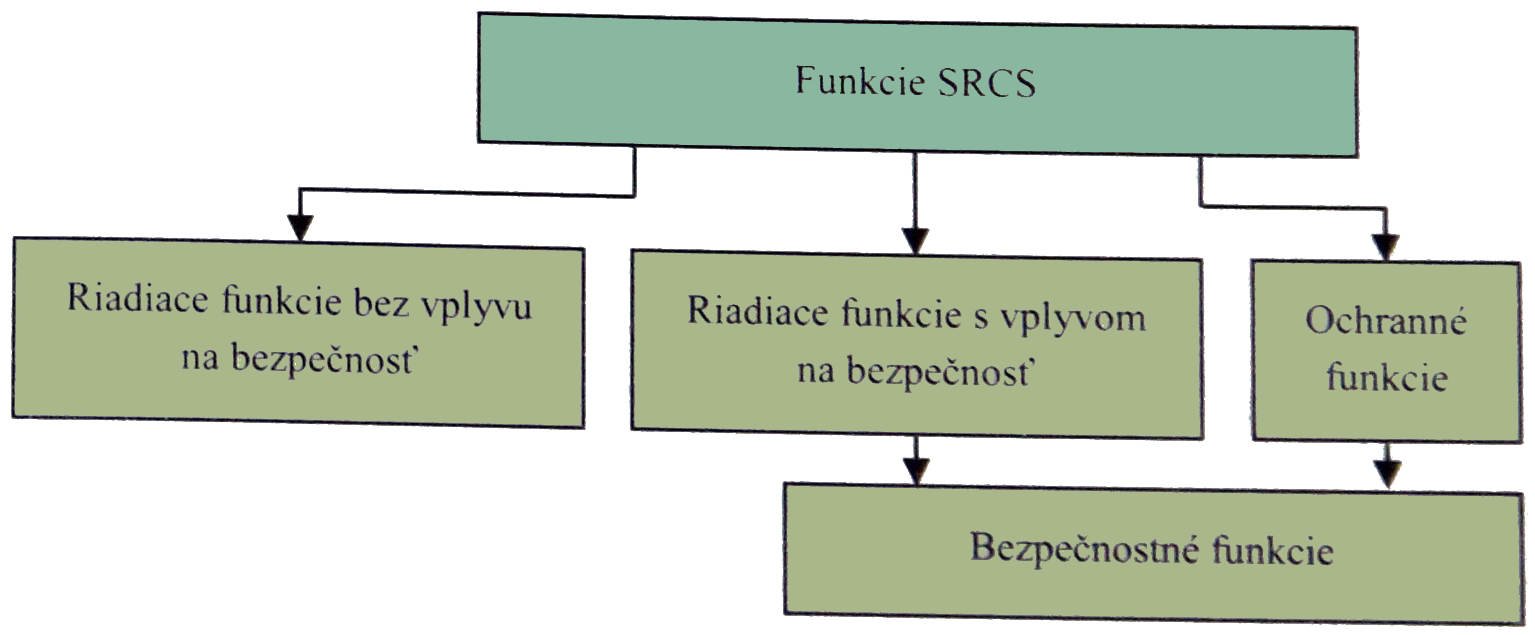
\includegraphics[width=1\linewidth]{DZT_SRCS_fce.jpg}
      \caption{Vztah mezi bezpečnostními funkcemi a moduly SRCS}
      \label{DZT:fig_DZT_SRCS_fce}
    \end{figure}    
    Bezpečnostní funkce jsou definované na základě analýzy rizik jako technická opatření na snížení
    rizika spojeného s konkrétními nebezpečí na tolerovatelnou úroveň. Účinnost bezpečnostní funkce
    se určuje pomocí úrovně integrity bezpečnosti \emph{(\texttt{SIL} - safety integrity level)}. 
    
    Norma \emph{EN 61508} definuje integritu bezpečnosti jako pravděpodobnost, že SRCS bude plnit 
    požadované bezpečné funkce za všech stanovených podmínek v rámci stanoveného operačního 
    prostředí a během stanoveného časového období. Všeobecně lze konstatovat, že čím je integrita
    bezpečnosti SRCS větší, tím je menší pravděpodobnost selhání bezpečností funkce realizovaných
    SRCS.  
    
    Integrita bezpečnosti se skládá ze dvou částí a to:
    \begin{itemize}
      \item \emph{integrity bezpečnosti proti systematickým poruchám}: jde o nekvantifikovatelnou
            část integrity bezpečnosti, která souvisí s nebezpečnými systematickými poruchami 
            hardware a software; integrity bezpečnosti proti systematickým poruchám se dosahuje
            především opatřeními na předcházení chybám a poruchám; vzhledem k tomu, že jde o 
            nekvantifikovatelnou část integrity bezpečnosti, je vhodnější chápat integritu 
            bezpečnosti jako vlastnost a né jako pravděpodobnost; hodnocení integrity bezpečnosti
            proti systematickým chybám a poruchám se realizuje kontrolou dodržování opatření
            předcházejících chybám a poruchám, mezi které patří také důsledné testování korektní
            realizace bezpečnostních funkcí; 
      \item \emph{integrity bezpečnosti proti náhodným poruchám}: jde o kvantifikovatelnou část
            integrity bezpečnosti, která se týká náhodných poruch hardware vyplývajících z konečné
            bezporuchovosti použitých součástek; hodnocení integrity bezpečnosti proti náhodným
            poruchám se realizuje prostřednictvím pravděpodobnostních výpočtů.
    \end{itemize}
    
    Aby se dosáhla požadovaná integrita bezpečnosti, musí být splněné požadavky na integritu proti 
    systematickým poruchám i náhodným poruchám. 
    
    \subsection{Úroveň integrity bezpečnosti}
      Úroveň integrity bezpečnosti (\emph{Safety Integrity Levels - \texttt{SIL}}) se dělí podle EN 
      50129
      do čtyř kategorií - úroveň 4 (\texttt{SIL} 4) je nejvyšší, úroveň 1 (\texttt{SIL} 1) je 
      nejnižší.  Pokud se
      objevuje úroveň \texttt{SIL} 0, značí to, že se jedná o systém na které nejsou kladeny žádné
      bezpečnostní požadavky (ve smyslu zabezpečovací techniky)
      
      Proto, aby SRCS mohl být zařazen do odpovídající úrovně bezpečnosti \texttt{SIL}, musí 
      vyhovovat
      těmto faktorům:
      \begin{itemize}
        \item naplnění podmínek řízení kvality, 
        \item naplnění podmínek řízené bezpečnosti,
        \item splnění požadavků na technickou bezpečnost, 
        \item dosažení kvantitativního cíle
      \end{itemize}
      
      Jak patrno, splnění kvantitativního ukazatele samo o sobě neznamená, že bylo dosaženo
      odpovídající úrovně bezpečnosti. To platí ovšem i naopak - splnění tří předchozích podmínek
      (řízení kvality, řízení bezpečnosti a technické bezpečnosti) nezaručuje, že bylo dosaženo
      kvantitativních cílů a nelze tedy tvrdit, že zařízení lze zařadit do odpovídající skupiny
      \texttt{SIL} (\ref{DZT:fig_EN50129_SIL_techniques}).
      
      \begin{figure}[ht!]% Relationship between \texttt{SIL}s and techniques
        \centering
        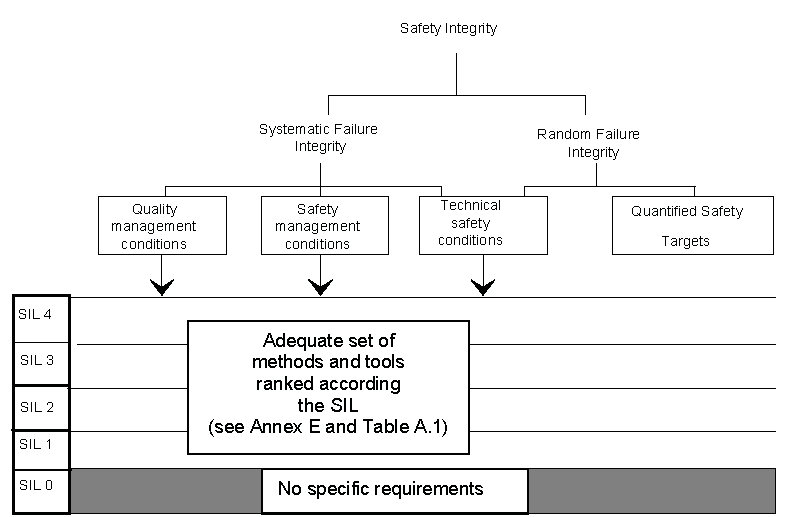
\includegraphics[width=0.95\linewidth]{EN50129_SIL_techniques.pdf}
        \caption{Vztah mezi \texttt{SIL} úrovní a technikami jejich dosažení}
        \label{DZT:fig_EN50129_SIL_techniques}
      \end{figure}
      
      Žádná z norem \texttt{CENELEC} nepředepisuje, které zařízení musí být jaké úrovně. Toto 
      určení je 
      ponecháno na provozovateli, resp. regulátorovi, vyplyne také z provedených analýz rizik 
      a hazardů.
      
      Následující tabulka shrnuje definované úrovně integrity bezpečnosti a zároveň dává do
      souvislosti s tolerovatelnými četnostmi hazardů. \texttt{SIL} jsou tedy prostředkem přiřazení
      kvalitativních přístupů (pro vyloučení systematických poruch) ke kvantitativnímu přístupu
      (pro řízení náhodných poruch), neboť systematické poruchy nelze kvantifikovat.
      \begin{table}[h]
        \centering
        \begin{tabular}{|c|c|}
          \hline
           Úroveň integrity &  Tolerovatelná četnost hazardu            \\
             bezpečnosti \texttt{SIL} &  THR [za hodinu a funkci]       \\ \hline\hline 
              4        & \(10^{-9}\leq THR < 10^{-8}\)                  \\ \hline
              3        & \(10^{-8}\leq THR < 10^{-7}\)                  \\ \hline
              2        & \(10^{-7}\leq THR < 10^{-6}\)                  \\ \hline
              1        & \(10^{-6}\leq THR < 10^{-5}\)                  \\ \hline
        \end{tabular}
        \caption{\texttt{SIL} tabulka: Funkce, jejichž kvantitativní požadavky by převyšovaly 
                 hranici \(10^{-9}\), která se zdánlivě nelogicky objevuje u \texttt{SIL4}, vyžaduje
                 podle normy \texttt{EN~50129} zvláštní technická nebo provozní opatření pro 
                 dosažení tak mimořádného cíle.}
      \end{table}
       
      \begin{enumerate}
        \item Z normy jasně vyplývá rozdělení na dvě skupiny \texttt{SIL 1,2} vs. \texttt{SIL 3,4}, 
              u nichž je výrazný rozdíl v požadavcích, které je potřeba splnit, aby SRCS mohl 
              patřit do dané skupiny. To je velmi dobře patrné z tabulek v příloze \texttt{E} normy 
              \texttt{EN 50129}, která se zabývá technikami a opatřeními pro řízení náhodných a 
              systematických poruch. 
        \item Druhým důležitým faktem je poněkud odlišná definice chápání úrovní \texttt{SIL} v 
              EN~61508. \emph{Funkční bezpečnost elektrických, elektronických, programovatelných
              elektronických systémů souvisejících s bezpečností}. Tato norma je obecnou normou pro
              průmyslové elektronické systémy, z níž vycházejí normy EN~50126, EN 50~129 atd.
              jakožto specifické normy pro železniční aplikace. Důležitou odlišností ve specifikaci
              \texttt{SIL}, viz tab. 2 a 3 v první části této normy (EN~61508-1). Nicméně tabulka 3 
              pro
              režim provozu s vysokým, resp. nepřetržitým vyžádáním odpovídá tabulce v normě
              EN~50129. Avšak i pro tyto systémy se zde jeví určitá odlišnost v požadavcích na
              zajištění dané \texttt{SIL}. Norma EN~61508 je zaměřena pouze na \emph{funkční 
              bezpečnost},
              není zde zahrnutý požadavek na bezpečnou reakci na ojedinělé náhodné poruchy. S
              poruchami se samozřejmě pracuje, mají být provedena opatření k jejich maximálnímu
              potlačení - četnosti i následku, nicméně může stačit, když systém je schopen poruchy
              detekovat a dát o nich vědět (např. obsluze). Závěrem nutno dodat, že je potřeba
              určité obezřetnosti k tvrzení, že systém splňuje daný \texttt{SIL}. Tento údaj musí 
              být
              doplněn specifikací, která norma byla při klasifikaci použita.
      \end{enumerate}
      
%\end{Czech}

%} %tikzset
%~~~~~~~~~~~~~~~~~~~~~~~~~~~~~~~~~~~~~~~~~~~~~~~~~~~~~~~~~~~~~~~~~~~~~~~~~~~~~~~~~~~~~~~~~~~~~~~~~~
\printbibliography[title={Seznam literatury}, heading=subbibliography]
\addcontentsline{toc}{section}{Seznam literatury}
}
{
 % DEBUG was off
%========== Kapitola 001: Bezpečnost a spolehlivost zabezpečovacích systémů =======================
  % !TeX spellcheck = cs_CZ
%{\tikzset{external/prefix={tikz/PZT/}}
% \tikzset{external/figure name/.add={ch02_}{}}
%---------------------------------------------------------------------------------------------------
% file ra3ch001.tex
%---------------------------------------------------------------------------------------------------
%======================== Kapitola: Železniční zabezpečovací technika ============================
%\begin{Czech}
\chapter{Obsah zabezpečovací techniky}\label{bzt:chapI}
\minitoc
  Důležitým odvětvím v železniční dopravě je odvětví zabezpečovací techniky. Potřeba zabezpečení 
  železničního provozu vznikala již v prvních začátcích železniční dopravy, ale postupný rozvoj 
  železniční dopravy si vynutil stále větší požadavky na konstrukci nových druhů zařízení a na 
  odbornost pracovníků pro jejich obsluhu.
  
  Tyto příručka je určena jako studijní materiál nezbytný pro implementaci moderních 
  metod návrhu zabezpečovacích systémů v železniční dopravě. 
   
\section{Náplň zabezpečovací techniky}
  Klasická železniční zabezpečovací zařízení jsou definována jako zařízení, která prvořadě 
  kontrolují, zda zamýšlené disposice dopravních zaměstnanců jsou bezpečné a zda jím nařízené 
  výkony se provádějí tak, aby nebyla ohrožena bezpečnost železniční dopravy. Pro přiblížení 
  uvažujme část stanice podle obr. \ref{zzt:fig001} a na této situaci s určitými zjednodušeními 
  tento obsah naznačme.

  \begin{figure}[ht!] %\ref{zzt:fig001}
    \centering
    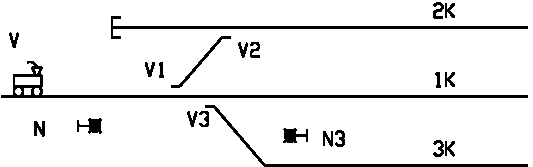
\includegraphics[width=0.8\linewidth]{zzt_fig001.pdf}
    \caption{Stanice
             (\cite[s.~5]{Chudacek2005})}
    \label{zzt:fig001}
  \end{figure}
 
  Před stanicí je umístěno návěstidlo \(N\), které v základní poloze ukazuje návěst \uv{stůj}. Dokud
  návěstidlo ukazuje tuto návěst, nesmí vlak \(V\) do stanice vjet. Má-li vlak vjet bezpečně např. 
  na kolej \(1K\), je třeba splnit určité podmínky. Výměny - pohyblivé části výhybek - \(V1\) a 
  \(V3\) musí být v poloze umožňující řádnou jízdu na kolej \(1K\), tj. jeden jazyk musí
  vždy přiléhat k příslušné opornici, druhý musí být od své opornice náležitě vzdálen. Na koleji 
  \(1K\) (včetně výhybek \(V1\) a \(V3\)) nesmí být žádná vozidla a ani nesmí být povolen příjezd
  jiných vozidel na tuto kolej z opačného směru. Zamýšlenou cestu nesmí ohrožovat z boku pohyby 
  jiných vlaků nebo posunujících dílů, proto výměna \(V2\) musí kolizní jízdu svou polohou 
  znemožňovat a návěstidlo \(N3\) musí kolizní jízdu zakazovat (ochrana odvratnou polohou výměny se 
  nazývá \emph{přímou boční ochranou}, ochrana návěstidlem se zakazující návěstí je \emph{nepřímou 
  boční ochranou}). Když tedy byly všechny prvky zvolené cesty správně nastaveny, přezkoušeny a 
  shledány bez závady, může být návěstidlo \(N\) přestaveno do polohy dovolující jízdu. Po celou 
  dobu, kdy návěstidlo dovoluje jízdu, bude dohlíženo, že všechny k tomu rozhodující podmínky jsou 
  nadále splněny. Vlak \(V\) vjede do stanice a ihned po jeho vjezdu se návěstidlo \(N\) přestaví 
  opět do základní polohy (návěst "stůj"), aby týž povel návěstidla nemohl být využit více vlaky a 
  aby shora uvedený postup bylo třeba pro každý vlak znovu opakovat.

  \begin{figure}[ht!] %\ref{zzt:fig002}
    \centering
    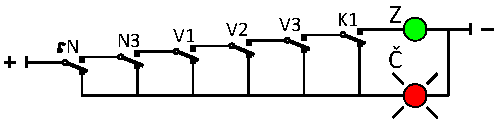
\includegraphics[width=0.8\linewidth]{zzt_fig002.pdf}
    \caption{Vybavení koleje technickým zařízením, které dohlíží na aby vlak vjel do stanice 
             bezpečně
             (\cite[s.~5]{Chudacek2005})}
    \label{zzt:fig002}
  \end{figure}
  
  Úkony, potřebné k tomu, aby vlak vjel do stanice bezpečně, může vykonat určený zaměstnanec. Ten
  se například pochůzkou přesvědčí, že kolej \(1K\) je volná, že výměny jsou řádně postaveny atd. a 
  po ověření všech podmínek přestaví návěstidlo \(N\) do polohy povolující jízdu. Pokud se 
  zaměstnanec nezmýlí, nedojde k nehodě (povšimněme si, že negace této věty nemusí být pravdivá). 
  Bezpečnost jízdy vlaku bude tedy závislá na osobních vlastnostech člověka. Aby tomu tak nebylo, 
  vybavíme koleje technickým zařízením, které bude na jejich volnost dohlížet, výměny jinými
  technickými zařízeními, která budou kontrolovat jejich polohu atd. a jízdní návěst návěstidel
  učiníme nuceně závislou na informacích těchto technických zařízení. Primitivní schéma
  takového zařízení je na obr. \ref{zzt:fig002}. I když pak dopravní zaměstnanec dá návěstním 
  řadičem \(N\) pokyn k rozsvícení jízdní (tj. jízdu povolující) návěsti \(Z\), návěst se rozsvítí 
  jen v případě, že kontakt \(N3\) informuje svým sepnutím, že návěstidlo \(N3\) skutečně ukazuje 
  návěst "stůj", kontakty \(V1\), \(V2\) a \(V3\) informují, že výměny jsou ve správné poloze a 
  kontakt \(K1\) informuje, že první kolej je volná a není na ni postavena jiná cesta. Jízdní 
  návěst \(Z\) se tedy rozsvítí až po splnění všech předem stanovených podmínek pro bezpečný vjezd 
  vlaku. Není-li kterákoliv podmínka splněna, na návěstidle \(N\) zůstává svítit červené světlo Č. 
  
  Přesto takové zařízení \textbf{nelze} považovat za zabezpečovací zařízení. Prvním důvodem je, že 
  nebyly zřízeny \emph{vzájemné závislosti}. Jízdní návěst na návěstidle \(N\) se sice rozsvítí až 
  když jsou splněny všechny podmínky, ale výměny a návěstidla zůstala volná. Nic nebrání, aby se 
  např. poloha výměn změnila dříve, než vlak \(V\) ukončí svou jízdu. Zhasnutí jízdního znaku \(Z\) 
  na návěstidle \(N\) v důsledku ztráty kontroly při přestavení výměny už nemusí být nic platné, 
  protože vlak již mohl návěstidlo minout nebo již není schopen včas zastavit. Nepostačí ale ani 
  zřízení vzájemné závislosti tím, že by rozsvícená jízdní návěst \(Z\) uzavírala výměny a 
  návěstidla v žádoucí poloze (např. prostřednictvím sériově řazeného relé). Vzhledem k nebezpečí
  přerušení sekvence postupných kroků je důležité, aby uzavření výměn a návěstidel bylo provedeno 
  dříve, než se rozsvítí jízdní návěst. Postup stavění jízdní cesty, vyhovující požadavkům 
  zabezpečovací techniky, bude tedy v naznačeném příkladě následující:
  \begin{itemize}\addtolength{\itemsep}{-0.5\baselineskip}
    \item nejprve se přestaví výměny do žádané polohy,
    \item v druhém úkonu (nazývaném závěr jízdní cesty) se při uzavírání výměn a návěstidel 
          přezkouší jejich správná poloha a tedy, že první úkon byl řádně proveden. Pokud první 
          úkon nebyl proveden správně, musí být znemožněn úkon druhý,
    \item obdobně třetí úkon, tj. rozsvícení jízdní návěsti na návěstidle \(N\), je možný jen 
          tehdy, byl-li druhý úkon (a tedy i první úkon) řádně proveden. 
  \end{itemize}
  
  Tím jsme dosáhli požadované \emph{vzájemné závislosti}, jejíž popsaná úroveň je \textbf{prvním
  charakteristickým rysem} zabezpečovacího zařízení. Zařízení z obr. \ref{zzt:fig002} bude podmínce 
  vyhovovat například v případě, že návěstní přepínač \(N\) bude konstrukčně upraven tak, že ho 
  nebude možné přeložit bez provedení \textbf{závěru jízdní cesty}. Důsledkem zavedení závěru 
  jízdní cesty bude potřeba po vlaku jízdní cestu vybavit, tj. závěr zrušit, aby bylo možné s 
  jednotlivými prvky opět volně manipulovat. 

  Ani nyní však ještě nelze v uvedeném příkladě hovořit o zabezpečovacím zařízení. Zařízení musí
  být konstruováno tak, aby \emph{bezpečnost byla zachována i při jakékoliv možné poruše vlastního 
  zařízení}. Tento  požadavek platí jak pro jednotlivé části, tak pro celek a je \textbf{druhým 
  charakteristickým rysem} železniční zabezpečovací techniky. V uvedeném případě to znamená, že 
  zařízení pro kontrolu volnosti koleje nesmí ani při poruše hlásit obsazenou kolej jako volnou, 
  zařízení pro kontrolu polohy výměny nesmí ani při poruše hlásit nesprávně postavenou výměnu jako 
  výměnu správně postavenou, ke zrušení závěru jízdní cesty nesmí ani poruchou dojít dříve než vlak 
  dotčené prvky skutečně mine atd. Právě tak vlastní zapojení pro rozsvícení jízdní návěsti musí 
  být konstruováno tak, aby se jízdní návěst nemohla poruchou zapojení rozsvítit, pokud všechny 
  podmínky pro její svícení nebudou splněny. Jak patrno, vychází se ze základního železničního
  bezpečnostního předpokladu, že zastavení vlaku poskytuje nejvyšší bezpečnost. Tento předpoklad se 
  zásadně liší od principů aplikovaných v letecké dopravě, kosmonautice, nukleární technice, 
  navigaci, řízení procesů, robotice, dolování, systémech zabezpečení proti vloupání či odcizení 
  atd., kde je prozatím obvykle hlavním cílem dosažení maximální spolehlivosti a pohotovosti 
  systému.
  
  Důsledkem druhého charakteristického rysu zabezpečovací techniky, tj. převedení všech poruch
  bezpečnějším směrem je, že téměř každá porucha zabezpečovacího zařízení znamená omezení dopravy. 
  To samozřejmě může vést k narušení plynulosti a vzniku provozních nepravidelností, což jsou jevy, 
  které samy o sobě nebezpečí v dopravě výrazně zvětšují. Ve vážnějších případech je nutné 
  zabezpečovací zařízení do skončení jeho opravy zcela vypnout, aby byl možný alespoň omezený pohyb 
  vlaků. Pak se ovšem provoz, jehož pravidelnost je navíc narušena, děje bez jakékoliv podpory 
  zabezpečovacího zařízení, zatížen, byť i jen na omezenou dobu, možnými lidskými omyly. Odtud tedy 
  plyne třetí charakteristický rys zabezpečovací techniky, což je taková konstrukce zařízení, která 
  má co nejméně poruch, tedy vysokou spolehlivost nebo - obecněji - co nejvyšší pohotovost. 
 
  Úloha zabezpečovací techniky nekončí zajištěním odpovídajícího návěstního znaku na návěstidle.
  Také na lokomotivě je strojvedoucí, jemuž je svěřena péče o bezpečnost vlaku a který tuto 
  bezpečnost může ohrozit svým omylem. Působnost zabezpečovacích zařízení se tedy (prostřednictvím 
  vlakového zabezpečovacího zařízení) prodlužuje až na vozidlo, aby se zajistilo, že vlak také 
  skutečně bude návěsti respektovat. 

  Aplikují-li se všechny výše uvedené zvláštnosti správně při vývoji zabezpečovacího systému, je
  třeba se postarat také o to, aby nedošlo k jejich znehodnocení při projekci, výrobě, montáži a 
  údržbě konkrétních zařízení. Při těchto činnostech je také třeba počítat s lidskými vlastnostmi. 
  Zařízení, sloužící primárně pro eliminaci chyb dopravních zaměstnanců konstruují, vyrábějí, 
  montují a udržují opět lidé. Naštěstí tyto práce, na rozdíl od výkonu dopravní služby, probíhají 
  (nebo by rozhodně měly probíhat) v lepších podmínkách a bez časové tísně. Za příznivých podmínek 
  se nedokonalosti člověka tolik neuplatňují a práci každého pracovníka lze kontrolovat jinými s 
  případnou pomocí dalších technických zařízení. Přesto však z toho pro projekci, výrobu, montáž a 
  údržbu zabezpečovacích zařízení vyplývají jisté zvláštnosti. 
  
  Vedle úloh z oblasti bezpečnosti plní moderní zabezpečovací technika i úkoly další. Především jde
  o hlubší zásahy do vlastního provozu prostředky automatizace. Ta pak, při správném provedení, 
  vede k zlepšenému využití technických prostředků železnic (např. zvýšení propustné výkonnosti 
  tratí), k zhospodárnění provozu, k úspoře jiných, podstatně vyšších investičních nákladů (např. 
  budování další koleje). Protože však zabezpečovací zařízení je zařízením v zásadě restriktivním, 
  nelze u něj bezhlavě prosazovat zvyšování výkonnosti vždy a ve všech směrech. Později také 
  uvidíme, že zabezpečovací technika se podílí na zvyšování bezpečnosti i v jiných oblastech: 
  kolejové obvody alespoň částečně dohlíží na stav jízdní dráhy (celistvost kolejnic), přestavná 
  zařízení výměn dohlíží na stav výhybek, vlakové zabezpečovače mohou do určité míry dohlížet na 
  stav brzdové soustavy vlaku (sledováním skutečně dosaženého odrychlení při brzdění), přejezdová 
  zabezpečovací zařízení se podílejí na eliminaci cizích vlivů na dopravu atd.
  
  Souhrnně lze konstatovat, že prvořadým účelem zabezpečovacích zařízení na železnici je
  předcházet kolizím a vykolejení vlaků z důvodu chybného řízení dopravy. K tomu účelu je u 
  zařízení třeba sledovat následující oblasti:
  \begin{itemize}\addtolength{\itemsep}{-0.5\baselineskip}
    \item funkční bezpečnost (korektnost systému), tj. řádné plnění všech požadovaných funkcí v 
          bezporuchovém stavu a při očekávaných vlivech pracovního prostředí,
    \item technickou bezpečnost (bezpečnou konstrukci), tj. splnění požadavku, aby nedošlo k 
          přímému ohrožení bezpečnosti dopravy ani při poruchách samotného zabezpečovacího zařízení,
    \item bezpečnou aplikaci, tj. vytvoření takových logických funkcí a vzájemných závislostí, aby 
          pro konkrétní situaci navržené zařízení ve všech provozních stavech mohlo řádně plnit 
          svou funkci (na jeho výstupech budou jízdu povolující informace pouze v takovém rozsahu, 
          který odpovídá stavu informací vstupních) a zajištění, aby tyto vlastnosti zařízení mělo 
          i po výrobě a montáži,
    \item bezpečný provoz a údržbu, tj. zajištění, že předchozí úrovně zůstanou v zařízení 
          zachovány po celou dobu životnosti,
    \item vysokou spolehlivost, tj. omezení případů, kdy nepřímo, vyřazením zabezpečovacího 
          zařízení a přechodem na manuální řízení, by mohlo dojít k ohrožení bezpečnosti dopravy.
  \end{itemize}
  Žádnou ze zmíněných oblastí nelze preferovat, protože žádná nemůže nahradit druhou a             
  nedostatky v kterékoliv z nich znehodnocují výsledky ostatních.
  
  Přímým obsahem železniční zabezpečovací techniky není zajištění zdraví a bezpečnosti
  zaměstnanců (i když provozovaná zařízení samozřejmě musí splňovat i požadavky např. ve směru 
  ochrany před nebezpečným dotykovým napětím, ergonomicky správně navrženého obsluhovací pracoviště 
  atd.), zabránit nehodám ze zlého úmyslu, násilnou obsluhou, úmyslným poškozením nebo zneužitím 
  zařízení. V poslední době se však jeví jako nezbytné dokonaleji zajišťovat zabezpečovací zařízení 
  proti vandalům a lapkům všeho druhu a neoprávněným zásahům do zařízení v případě, že používají 
  jiných než speciálně drážních zařízení (viz dále např. ochrana dat v otevřených sítích).  

\section{Třídění}
  K železničním zabezpečovacím zařízením se obvykle řadí i zabezpečovací zařízení používaná na
  podzemních drahách (metro, doly), na pouličních drahách (tramvaje - zejména městské rychlodráhy) 
  a na vlečkách, protože využívají obdobných principů, často i obdobná nebo jen poněkud upravená 
  zařízení. Při třídění zařízení lze použít řadu třídících hledisek; téměř vždy se však vyskytnou 
  zařízení přechodová (smíšená) nebo podle užitého třídění obtížně definovatelná. Přesto je dále 
  několik třídění uvedeno, protože poskytují obrázek o pestrosti a mnohotvárnosti pojednávaného 
  zařízení. 
  
  Nejpřirozenějším a klasickým tříděním zabezpečovacích zařízení je třídění podle účelu zařízení.
  Podle tohoto hlediska lze zabezpečovací zařízení dělit na zařízení: 
  \begin{itemize}\addtolength{\itemsep}{-0.5\baselineskip}
    \item staniční,
    \item traťové,
    \item vlakové,
    \item přejezdové, 
    \item spádovištní. 
  \end{itemize}
  Účel je patrný již z názvu. Staniční zabezpečovací zařízení zajišťuje bezpečný pohyb vlaků ve 
  stanici, traťové zařízení zabezpečuje jízdu vlaku na trati mezi stanicemi, vlakové zařízení 
  zabraňuje vlaku pohybovat se nad rámec, který povoluje zařízení staniční a traťové (s případným 
  zahrnutím i dalších omezení), přejezdové zařízení přispívá k zajištění bezpečnosti na úrovňovém 
  křížení silnice a železnice informováním uživatelů silnice, že se k přejezdu blíží vlak s 
  předností v jízdě. Nad všemi těmito zařízeními pak může být budováno zařízení pro dálkové 
  ovládání většího úseku tratě z jednoho místa. 
  
  Podle místa ovládání zařízení mluvíme o zařízení s obsluhou :
    \begin{itemize}\addtolength{\itemsep}{-0.5\baselineskip}
    \item místní,
    \item ústřední (centralizovanou v oblasti jedné stanice),
    \item dálkovou (mimo vlastní stanici).
  \end{itemize}

  Další třídění je odvozeno od způsobu ovládání periferií (výměn, návěstidel atd.) a tak vlastně
  zahrnuje celou historii železniční zabezpečovací techniky. Rozeznáváme zařízení:
  \begin{itemize}\addtolength{\itemsep}{-0.5\baselineskip}
    \item mechanická (využívající výhradně lidské síly),
    \item elektrická,
    \item pneumatická,
    \item hydraulická. 
  \end{itemize}

  Obdobně, v následujícím třídění je rozhodující způsob, jímž se v zařízení potřebné závislosti
  realizují. Zde rozeznáváme zařízení se závislostmi:
  \begin{itemize}\addtolength{\itemsep}{-0.5\baselineskip}
    \item mechanickými,
    \item mechanickými i elektrickými (tzv. elektromechanická a elektrodynamická zařízení),
    \item elektrickými, která lze dále dělit podle rozhodujících stavebních prvků, jimiž jsou 
         závislosti realizovány, na zařízení:
       \begin{itemize}
       \item reléová,
       \item hybridní (rozhodující část bezpečné logiky je realizována reléově, zbytek 
             elektronicky),
       \item elektronická (mikroprocesorová). 
       \end{itemize}
  \end{itemize}

  U traťových zabezpečovacích zařízení je kladen důraz na rozsah spolupůsobení vlaku. Zařízení se
  pak dělí na:
  \begin{itemize}\addtolength{\itemsep}{-0.5\baselineskip}
    \item poloautomatická (poloautobloky),
    \item automatická (autobloky).
  \end{itemize}
  Podle rozmístění traťových zařízení podél trati lze automatická zařízení dále dělit na:
  \begin{itemize}\addtolength{\itemsep}{-0.5\baselineskip}
    \item decentralizovaná (funkční bloky jsou umístěny v každém návěstním bodě),
    \item částečně centralizovaná (funkční bloky jsou umístěny pouze ve vybraných bodech na trati),
    \item centralizovaná (zařízení je koncentrováno do stanic).
  \end{itemize}
  Vlaková zabezpečovací zařízení se dělí podle způsobu přenosu informací mezi tratí a hnacím
  vozidlem na zařízení:
  \begin{itemize}\addtolength{\itemsep}{-0.5\baselineskip}
    \item bodová,
    \item semiliniová,
    \item liniová. 
  \end{itemize}

  Podle způsobu kontroly souladu jízdy vlaku s přenášenými informacemi se vlaková zařízení dále 
  dělí na zařízení s kontrolou:
  \begin{itemize}\addtolength{\itemsep}{-0.5\baselineskip}
    \item bdělosti strojvedoucího,
    \item rychlosti vlaku.
  \end{itemize}
  
  Zařízení přejezdová se dělí podle způsobu výstrahy na přejezdová zařízení:
  \begin{itemize}\addtolength{\itemsep}{-0.5\baselineskip}
    \item mechanická,
    \item světelná bez závor,
    \item světelná se závorami.
  \end{itemize}
  
  U moderních systémů dělení zabezpečovacích zařízení na zařízení staniční, traťová, vlaková a
  přejezdová ztrácí smysl, protože systémy jsou komplexní, se společným jádrem řídícím jednotlivé 
  periférie a tyto celky pak tvoří nanejvýš podsystémy. Na obr. 3-1 je základní blokové schéma 
  takového systému. 
  \begin{figure}[ht!] %\ref{zzt:fig003}
    \centering
    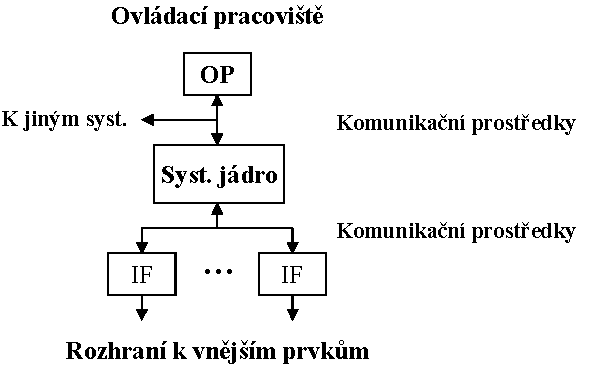
\includegraphics[width=0.8\linewidth]{zzt_fig003.pdf}
    \caption{Stanice
             (\cite[s.~11]{Chudacek2005})}
    \label{zzt:fig003}
  \end{figure}


  \section{Klasifikace poruch}
    \textbf{Chyba} je rozdíl mezi správnou a skutečnou hodnotou nějaké veličiny. V zařízení se 
    chyby mohou obecně objevit jako \emph{důsledek (projev) poruchy některé jeho součásti, 
    působením nějakého cizího vlivu} nebo \emph{selháním lidského činitele}. Za poruchy hardware se 
    považují všechna vybočení z předpokládaných vlastností stavebního prvku (součástky, dílu) 
    zařízení. Předpokládanými vlastnostmi prvků přitom jsou vlastnosti odpovídající příslušným 
    technickým podmínkám popisujícím jeho vlastnosti. Jako omyl lze označit každou lidskou činnost, 
    která může vést k nezamýšlenému chování zařízení. V širším slova smyslu se jako 
    \textbf{porucha} označují souhrnně všechny příčiny vedoucí k chybě, tj. poruch součásti, 
    cizí vliv i omyl.

%~~~~~~~~~~~~~~~~~~~~~~~~~~~~~~~~~~~~~~~~~~~~~~~~~~~~~~~~~~~~~~~~~~~~~~~~~~~~~~~~~~~~~~~~~~~~~~~~~~
\printbibliography[title={Seznam literatury}, heading=subbibliography]
\addcontentsline{toc}{section}{Seznam literatury}

\chapter{Bezpečnost a spolehlivost zabezpečovacích systémů}
 \section{Spolehlivost}
 \section{Bezpečnost}
    V různých publikacích je možné najít různé definice bezpečnosti. Například norma 
    EN~61508\footnote{Funkční bezpečnost elektrických/elektronických/programovatelných 
    elektronických systémů souvisejících s bezpečností (Functional safety of electrical/ 
    electronic/programmable electronic systems), obecná norma funkční bezpečnosti, která se opírá o 
    dvě základní koncepce - životní cyklus bezpečnosti a úroveň integrity bezpečnosti 
    (\texttt{SIL})} 
    definuje bezpečnost jako nepřítomnost netolerovaného rizika. Z této definice je zřejmé, že 
    bezpečnost je úzce spjatá s rizikem, a je nutné bezpečnost třeba chápat relativně. Když se 
    řekne, že řídicí systém je bezpečný, neznamená to jeho absolutní bezpečnost (ta je prakticky 
    nedosažitelná vzhledem na existenci objektivních faktorů, jako je například úroveň poznání, 
    technologická úroveň a limitované finanční prostředky), ale taková úroveň bezpečnosti, 
    která zodpovídá definovaným bezpečnostním požadavkům na tento řídicí systém. 

    Relativnost v pojímání bezpečnosti znamená posun od kvalitativního ke kvantitativnímu chápaní bezpečnosti.

    Kvalitativně je bezpečnost chápána jako schopnost řídicího systému zajistit omezení důsledků 
    poruch řídicích systému v daných podmínkách a v daném časovém intervalu. Matematicky je možné 
    kvalitativní bezpečnost řídicího systému vyjádřit jako 
    \begin{equation}
      E_H = 0,
    \end{equation}
    kde \(E_H\) je množina nebezpečných stavů, které jsou důsledkem výskytu pravděpodobných poruch 
    řídicího systému. Pravděpodobná porucha je taková porucha z množiny všech poruch, jejichž 
    výskyt během provozu řídicího systému je nutné předpokládat (vzhledem na požadovanou úroveň 
    bezpečnosti řídicího systému).
	
    Kvantitativně je bezpečnost řídicího systému chápána jako pravděpodobnost nepřítomnosti
    jakéhokoliv nebezpečného stavu v řídicím systému v daných podmínkách a v daném časovém
    intervalu. Je zřejmé, že i když pravděpodobnost nebezpečného stavu řídicího je malá, neznamená
    to, že se nebezpečný stav nemůže vyskytnou v nejbližším časovém intervalu, Matematicky je možné
    kvantitativní bezpečnost vyjádřit tak, že
    \begin{equation}
      P_{HT}(t)\geq P_{HT}(t)>0,
    \end{equation}
    kde \(P_{HT}(t)\) je pravděpodobnost tolerovaného nebezpeční řídicího systému a \(P_{HR}(t)\)
    je reálná pravděpodobnost nebezpeč\-ného stavu řídicího systému.
	 
    Na kvantitativním hodnocení bezpečnosti řídicího systému je v podstatě možné uplatnit stejné 
    teoretické postupy, jako při hodnocení spolehlivosti technických systémů. Zásadní rozdíl je v 
    tom, že při hodnocení spolehlivosti standardních řídicích systémů se obvykle rozlišují dva 
    stavy - bezporuchový stav a poruchový stav, a k těmto dvěma stavům se vztahují také 
    kvantitativní ukazatele spolehlivosti. Při hodnocení bezpečnosti řídicích systémů musíme 
    uvažovat s dvěma druhy poruchových stavů - bezpečným a nebezpečným poruchovým stavem. 
    Bezpečnost řídicího systému se potom vyjadřuje pomocí ukazatelů bezpečnosti (například 
    pravděpodobnost výskytu nebezpečné poruchy, intenzita nebezpečných poruch, ...).

    Při kvantitativním hodnocení důsledků poruch na bezpečnost řídicího systému se obvykle k 
    hodnoceným řídicím systémům přistupuje jako k neobnovovaným objektům, protože z pohledu 
    bezpečnosti jsou důležité dva stavy (bezpečný, nebezpečný) a analýza končí výskytem nebezpečné 
    poruchy (může jít o jednu poruchu, nebo o kombinaci více poruch, které nejsou individuálně 
    nebezpečné). To znamená, že od uvedení řídicího systému do provozu, až po výskyt nebezpečné 
    poruchy, se může řídicí systém střídavě nacházet ve funkčním, nebo nefunkčním stavu (nefunkční 
    ještě neznamená nebezpečný). Z tohoto důvodu ukazatele bezpečnosti jsou podobné ukazatelům 
    bezporuchovosti neobnovovaných objektů. 
  
    \subsection{Základní legislativa}
      \begin{itemize}
        \item \textbf{EN 61508} - \emph{základní všeobecná norma pro SRCS}; pojednává o funkční
              bezpečnosti elektrických/elektronických/programovatelných elektronických systémů
              souvisejících s bezpečností (Functional safety of electrical/electronic/programmable
              electronic systems), obecná norma funkční bezpečnosti, která se opírá o dvě základní
              koncepce - životní cyklus bezpečnosti a úroveň integrity bezpečnosti (\texttt{SIL})
              \begin{itemize}
                \item EN 61508-1: Všeobecné požadavky
                \item EN 61508-2: Požadavky na elektrické / elektronické / programovatelné
                                  elektronické systémy související s bezpečností
                \item EN 61508-3: Požadavky na SW
                \item EN 61508-4: Definice a zkratky
                \item EN 61508-5: Příklady metod určování úrovně integrity bezpečnosti
                \item EN 61508-6: Metodické pokyny na používání EN 61508-2, STN EN 61508-3
                \item EN 61508-7: Přehled technik a opatření
              \end{itemize}
        \item \textbf{EN 50126}: Railway applications – The specification and demonstration of
              reliability, availability, maintainability and safety (RAMS)
              \begin{itemize}
                \item Part 1: Basic requirements and generic process. 1999
                \item Part 2: Guide to the application of EN 50126-1 for safety. 2007
                \item Part 3: Guide to the application of EN 50126-1 for rolling stock RAMS. 2008  
              \end{itemize}
              Zabývá se specifikací parametrů RAMS (spolehlivost, pohotovost, udržovatelnost,
              a bezpečnost) obecně pro všechny železniční systémy, reaguje na skutečnost, že
              naléhavost požadavků na bezpečnost funkce jednotlivých železničních systémů je různá
              a lze je tedy splňovat s různou pravděpodobností jejich selhání. Také zavádí pojem
              \emph{integrita bezpečnosti (safety integrity - celistvost, úplnost, neporušenost
              bezpečnosti)}, který definuje jako pravděpodobnost, s níž systém uspokojivě splní
              požadované bezpečnostní funkce, za všech stanovených podmínek a ve stanoveném časovém
              období. Jde o to, do jaké míry může být pro bezpečnost relevantní funkce narušena
              např. poruchami vlastního zařízení, omyly obsluhy, vnějším rušením atd.
        \item \textbf{EN 50128}: Railway applications – Communication, signalling and processing
              systems – Software for railway control and protection systems. 2003          
        \item \textbf{EN 50129}: Railway applications – Communication, signalling and processing
              systems – Safety-related electronic systems for signalling. 2011
              Modifikovaně byl pojem integrita bezpečnosti přenesen i do této normy pro železniční
              zabezpečovací systémy. I klasická zabezpečovací technika bez velkého zdůrazňování
              respektovala, že nejsou na všechna zařízení kladeny stejně důrazné bezpečnostní
              požadavky (kategorie zařízení, vedlejší tratě/hlavní tratě, zařízení pro ČD/zařízení
              pro vlečky, staniční zařízení/spádoviště atd.). Uvidíme dále, že pojmu integrita
              bezpečnosti je pro zabezpečovací zařízení dominantně obsažena oblast, kterou běžně v
              této technice označujeme(a také normá EN 50129 ji tak označuje ve své základní části)
              termínem technická bezpečnost. Úvahy okolo integrity bezpečnosti zde sledujeme
              odděleně od úvah o technické bezpečnosti (přes jejich podobnost) pro jejich výhodnost
              zejména v úvodních fázích projektu nového systému (zařízení, výrobku, atd.)
        \item \textbf{EN 50159: Railway applications – Communication, signalling and processing
              systems - Safety-related communication in transmission systems. 2010}            
      \end{itemize}
    
      Vyjmenované normy se poněkud liší v definici termínu \emph{bezpečnost}:  
      \begin{itemize}
        \item Bezpečnost (Safety) – nepřítomnost nepřijatelných úrovní rizika poškození (EN50129)
        \item Bezpečnost (Safety) – nepřítomnost nepřijatelného rizika. (EN61508)
        \item Bezpečnost při poruše (Fail Safe) – vlastnost konstrukce objektu zabraňující,
              aby jeho poruchy způsobili nebezpečné poruchové stavy. (IEC 50 (191))
        \item Kvalitativní bezpečnost – schopnost systému zajistit omezení důsledku poruch
              systému v daných podmínkách a v daném časovém intervale.
        \item Kvantitativní bezpečnost – pravděpodobnost nepřítomnosti jakéhokoliv
              nebezpečného stavu v systéme v daných podmínkách a v daném časovém intervale.
      \end{itemize}

    \subsection{Ukazatel bezpečnosti}
      \fbox{Pravděpodobnost bezpečného provozu} je pravděpodobnost, že objekt může bezpečně plnit 
      požadovanou funkci v daných podmínkách v časovém intervalu \(t_1,\, t_2\).
      \begin{equation}
        R_S(t_1,\, t_2) = 1- F_H(t_1,\, t_2),
      \end{equation}
      kde \(F_H(t_1,\, t_2)\) je distribuční funkce, která naopak vyjadřuje pravděpodobnost, že
      objekt nemůže bezpečně plnit požadovanou funkci k daným podmínkám v časovém intervalu
      \(t_1,\, t_2\).
      \begin{equation}
        F_H(t_1,\, t_2) = \int_{t_1}^{t_2}f_H(t)\cdot\dd{t},
      \end{equation}
      kde \(f_H(t)\) je hustota pravděpodobnosti nebezpečné poruchy objektu. 

      \fbox{Intenzita nebezpečných poruch} \(\lambda_H(t)\) definujme jako limitu poměru podmíněné
      pravděpodobnosti, že časový okamžik vzniku nebezpečné poruchy objektu \(T\) padne do daného
      časového intervalu \(t,\, t+\Delta t\), přičemž délka časového intervalu \(\Delta
      t\rightarrow0\)
      \begin{equation}\label{DZT:eq_def_lambdaH}
        \lambda_H=\frac{f_H(t)}{R_S(t)}.
      \end{equation}

      Protože nebezpečné poruchy jsou méně časté, zkoušky na určení požadovaných ukazatelů
      bezpečnosti by bylo třeba provádět dlouhodobě, což je prakticky nemožné. 
    
  \section{Integrita bezpečnosti}
    Všeobecně je možné konstatovat, že SRCS realizuje řídící i ochranné funkce (obr.
    \ref{DZT:fig_DZT_SRCS_fce}). Jelikož selhání řídicí funkce může způsobit ohrožení bezpečnosti,
    je třeba i tyto funkce považovat za bezpečnostní.
    \begin{figure}[hb!]
      \centering
      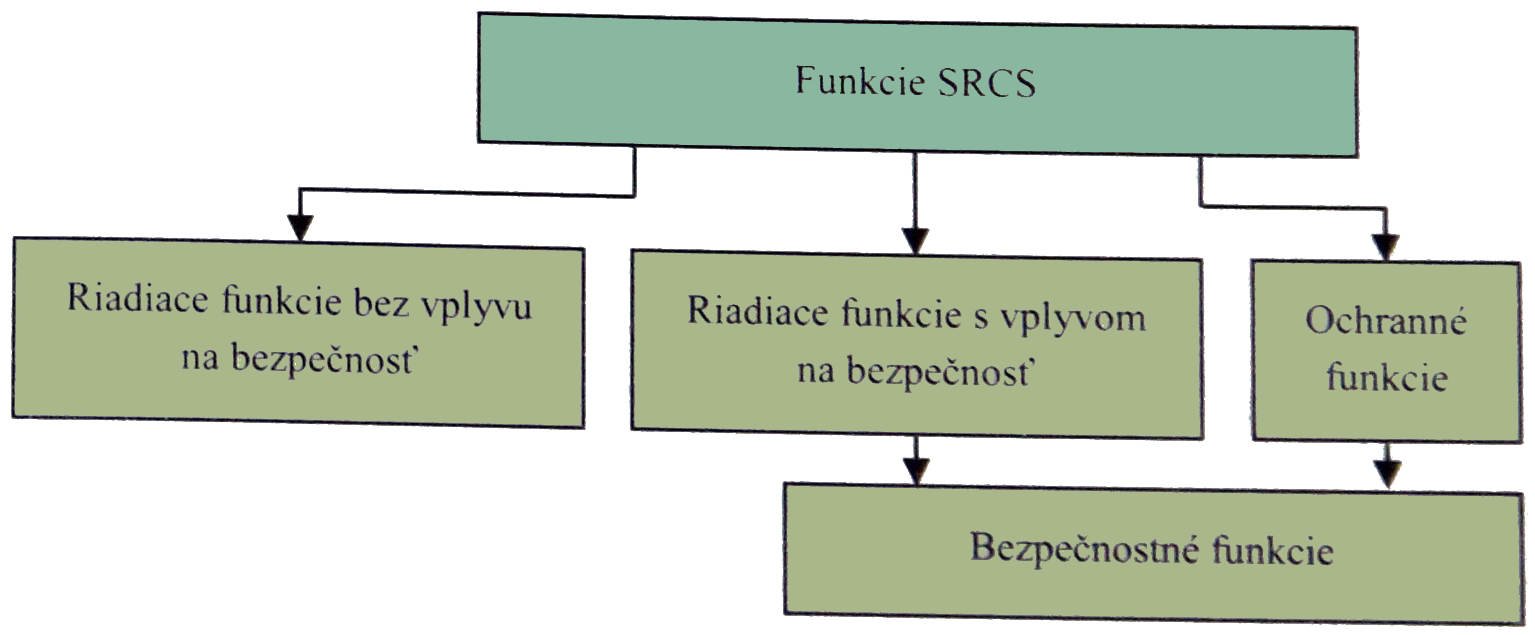
\includegraphics[width=1\linewidth]{DZT_SRCS_fce.jpg}
      \caption{Vztah mezi bezpečnostními funkcemi a moduly SRCS}
      \label{DZT:fig_DZT_SRCS_fce}
    \end{figure}    
    Bezpečnostní funkce jsou definované na základě analýzy rizik jako technická opatření na snížení
    rizika spojeného s konkrétními nebezpečí na tolerovatelnou úroveň. Účinnost bezpečnostní funkce
    se určuje pomocí úrovně integrity bezpečnosti \emph{(\texttt{SIL} - safety integrity level)}. 
    
    Norma \emph{EN 61508} definuje integritu bezpečnosti jako pravděpodobnost, že SRCS bude plnit 
    požadované bezpečné funkce za všech stanovených podmínek v rámci stanoveného operačního 
    prostředí a během stanoveného časového období. Všeobecně lze konstatovat, že čím je integrita
    bezpečnosti SRCS větší, tím je menší pravděpodobnost selhání bezpečností funkce realizovaných
    SRCS.  
    
    Integrita bezpečnosti se skládá ze dvou částí a to:
    \begin{itemize}
      \item \emph{integrity bezpečnosti proti systematickým poruchám}: jde o nekvantifikovatelnou
            část integrity bezpečnosti, která souvisí s nebezpečnými systematickými poruchami 
            hardware a software; integrity bezpečnosti proti systematickým poruchám se dosahuje
            především opatřeními na předcházení chybám a poruchám; vzhledem k tomu, že jde o 
            nekvantifikovatelnou část integrity bezpečnosti, je vhodnější chápat integritu 
            bezpečnosti jako vlastnost a né jako pravděpodobnost; hodnocení integrity bezpečnosti
            proti systematickým chybám a poruchám se realizuje kontrolou dodržování opatření
            předcházejících chybám a poruchám, mezi které patří také důsledné testování korektní
            realizace bezpečnostních funkcí; 
      \item \emph{integrity bezpečnosti proti náhodným poruchám}: jde o kvantifikovatelnou část
            integrity bezpečnosti, která se týká náhodných poruch hardware vyplývajících z konečné
            bezporuchovosti použitých součástek; hodnocení integrity bezpečnosti proti náhodným
            poruchám se realizuje prostřednictvím pravděpodobnostních výpočtů.
    \end{itemize}
    
    Aby se dosáhla požadovaná integrita bezpečnosti, musí být splněné požadavky na integritu proti 
    systematickým poruchám i náhodným poruchám. 
    
    \subsection{Úroveň integrity bezpečnosti}
      Úroveň integrity bezpečnosti (\emph{Safety Integrity Levels - \texttt{SIL}}) se dělí podle EN 
      50129
      do čtyř kategorií - úroveň 4 (\texttt{SIL} 4) je nejvyšší, úroveň 1 (\texttt{SIL} 1) je 
      nejnižší.  Pokud se
      objevuje úroveň \texttt{SIL} 0, značí to, že se jedná o systém na které nejsou kladeny žádné
      bezpečnostní požadavky (ve smyslu zabezpečovací techniky)
      
      Proto, aby SRCS mohl být zařazen do odpovídající úrovně bezpečnosti \texttt{SIL}, musí 
      vyhovovat
      těmto faktorům:
      \begin{itemize}
        \item naplnění podmínek řízení kvality, 
        \item naplnění podmínek řízené bezpečnosti,
        \item splnění požadavků na technickou bezpečnost, 
        \item dosažení kvantitativního cíle
      \end{itemize}
      
      Jak patrno, splnění kvantitativního ukazatele samo o sobě neznamená, že bylo dosaženo
      odpovídající úrovně bezpečnosti. To platí ovšem i naopak - splnění tří předchozích podmínek
      (řízení kvality, řízení bezpečnosti a technické bezpečnosti) nezaručuje, že bylo dosaženo
      kvantitativních cílů a nelze tedy tvrdit, že zařízení lze zařadit do odpovídající skupiny
      \texttt{SIL} (\ref{DZT:fig_EN50129_SIL_techniques}).
      
      \begin{figure}[ht!]% Relationship between \texttt{SIL}s and techniques
        \centering
        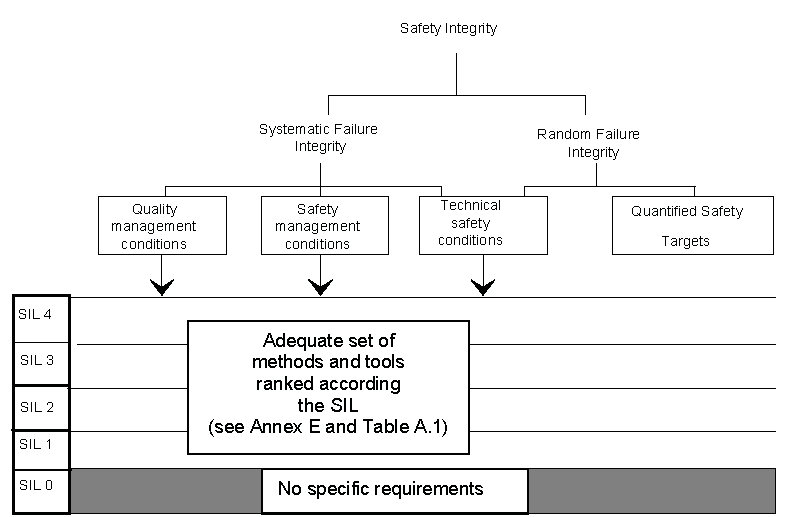
\includegraphics[width=0.95\linewidth]{EN50129_SIL_techniques.pdf}
        \caption{Vztah mezi \texttt{SIL} úrovní a technikami jejich dosažení}
        \label{DZT:fig_EN50129_SIL_techniques}
      \end{figure}
      
      Žádná z norem \texttt{CENELEC} nepředepisuje, které zařízení musí být jaké úrovně. Toto 
      určení je 
      ponecháno na provozovateli, resp. regulátorovi, vyplyne také z provedených analýz rizik 
      a hazardů.
      
      Následující tabulka shrnuje definované úrovně integrity bezpečnosti a zároveň dává do
      souvislosti s tolerovatelnými četnostmi hazardů. \texttt{SIL} jsou tedy prostředkem přiřazení
      kvalitativních přístupů (pro vyloučení systematických poruch) ke kvantitativnímu přístupu
      (pro řízení náhodných poruch), neboť systematické poruchy nelze kvantifikovat.
      \begin{table}[h]
        \centering
        \begin{tabular}{|c|c|}
          \hline
           Úroveň integrity &  Tolerovatelná četnost hazardu            \\
             bezpečnosti \texttt{SIL} &  THR [za hodinu a funkci]       \\ \hline\hline 
              4        & \(10^{-9}\leq THR < 10^{-8}\)                  \\ \hline
              3        & \(10^{-8}\leq THR < 10^{-7}\)                  \\ \hline
              2        & \(10^{-7}\leq THR < 10^{-6}\)                  \\ \hline
              1        & \(10^{-6}\leq THR < 10^{-5}\)                  \\ \hline
        \end{tabular}
        \caption{\texttt{SIL} tabulka: Funkce, jejichž kvantitativní požadavky by převyšovaly 
                 hranici \(10^{-9}\), která se zdánlivě nelogicky objevuje u \texttt{SIL4}, vyžaduje
                 podle normy \texttt{EN~50129} zvláštní technická nebo provozní opatření pro 
                 dosažení tak mimořádného cíle.}
      \end{table}
       
      \begin{enumerate}
        \item Z normy jasně vyplývá rozdělení na dvě skupiny \texttt{SIL 1,2} vs. \texttt{SIL 3,4}, 
              u nichž je výrazný rozdíl v požadavcích, které je potřeba splnit, aby SRCS mohl 
              patřit do dané skupiny. To je velmi dobře patrné z tabulek v příloze \texttt{E} normy 
              \texttt{EN 50129}, která se zabývá technikami a opatřeními pro řízení náhodných a 
              systematických poruch. 
        \item Druhým důležitým faktem je poněkud odlišná definice chápání úrovní \texttt{SIL} v 
              EN~61508. \emph{Funkční bezpečnost elektrických, elektronických, programovatelných
              elektronických systémů souvisejících s bezpečností}. Tato norma je obecnou normou pro
              průmyslové elektronické systémy, z níž vycházejí normy EN~50126, EN 50~129 atd.
              jakožto specifické normy pro železniční aplikace. Důležitou odlišností ve specifikaci
              \texttt{SIL}, viz tab. 2 a 3 v první části této normy (EN~61508-1). Nicméně tabulka 3 
              pro
              režim provozu s vysokým, resp. nepřetržitým vyžádáním odpovídá tabulce v normě
              EN~50129. Avšak i pro tyto systémy se zde jeví určitá odlišnost v požadavcích na
              zajištění dané \texttt{SIL}. Norma EN~61508 je zaměřena pouze na \emph{funkční 
              bezpečnost},
              není zde zahrnutý požadavek na bezpečnou reakci na ojedinělé náhodné poruchy. S
              poruchami se samozřejmě pracuje, mají být provedena opatření k jejich maximálnímu
              potlačení - četnosti i následku, nicméně může stačit, když systém je schopen poruchy
              detekovat a dát o nich vědět (např. obsluze). Závěrem nutno dodat, že je potřeba
              určité obezřetnosti k tvrzení, že systém splňuje daný \texttt{SIL}. Tento údaj musí 
              být
              doplněn specifikací, která norma byla při klasifikaci použita.
      \end{enumerate}
      
%\end{Czech}

%} %tikzset
%~~~~~~~~~~~~~~~~~~~~~~~~~~~~~~~~~~~~~~~~~~~~~~~~~~~~~~~~~~~~~~~~~~~~~~~~~~~~~~~~~~~~~~~~~~~~~~~~~~
\printbibliography[title={Seznam literatury}, heading=subbibliography]
\addcontentsline{toc}{section}{Seznam literatury}
} % DEBUG was off

%==================================================================================================
\setpartpreamble[u]{
\begin{center}
  \vspace{1cm}
  \Huge \uppercase{\textbf{Prvky}} \\
  \Huge \uppercase{\textbf{Železniční techniky}} \\
  \vspace{2cm}
  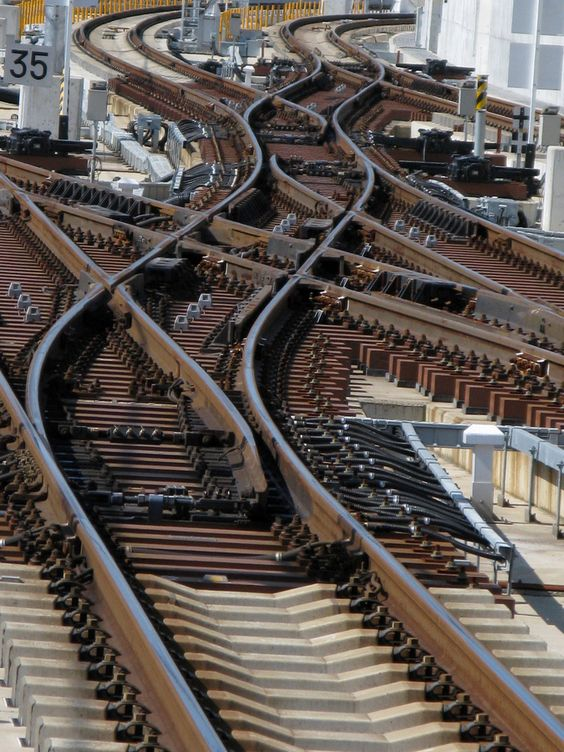
\includegraphics[width=0.8\linewidth]{PZT.jpg}
\end{center}
}

\part{PZT}\label{part:PZT}
\parttoc

\ifthenelse{ \equal{\DebugMode}{true} }{
% Debug mode ON
  % !TeX spellcheck = cs_CZ
%{\tikzset{external/prefix={tikz/PZT/}}
% \tikzset{external/figure name/.add={ch01_}{}}
%---------------------------------------------------------------------------------------------------
% file ra3ch001.tex
%---------------------------------------------------------------------------------------------------
%====================Kapitola: Výhybky =============================================================
\chapter{Výhybka}\label{pzt:chapI}
\minitoc

%} %tikzset
%~~~~~~~~~~~~~~~~~~~~~~~~~~~~~~~~~~~~~~~~~~~~~~~~~~~~~~~~~~~~~~~~~~~~~~~~~~~~~~~~~~~~~~~~~~~~~~~~~~
\printbibliography[title={Seznam literatury}, heading=subbibliography]
\addcontentsline{toc}{section}{Seznam literatury}

  % !TeX spellcheck = cs_CZ
%{\tikzset{external/prefix={tikz/PZT/}}
% \tikzset{external/figure name/.add={ch02_}{}}
%---------------------------------------------------------------------------------------------------
% file ra3ch001.tex
%---------------------------------------------------------------------------------------------------
%====================Kapitola: Detekce kolejových vozidel ==========================================
\chapter{Detekce kolejových vozidel}\label{pzt:chapII}
\minitoc

%} %tikzset
%~~~~~~~~~~~~~~~~~~~~~~~~~~~~~~~~~~~~~~~~~~~~~~~~~~~~~~~~~~~~~~~~~~~~~~~~~~~~~~~~~~~~~~~~~~~~~~~~~~
\printbibliography[title={Seznam literatury}, heading=subbibliography]
\addcontentsline{toc}{section}{Seznam literatury}

  % !TeX spellcheck = cs_CZ
%{\tikzset{external/prefix={tikz/PZT/}}
% \tikzset{external/figure name/.add={ch03_}{}}
%---------------------------------------------------------------------------------------------------
% file ra3ch001.tex
%---------------------------------------------------------------------------------------------------
%====================Kapitola: Detekce kolejových vozidel ==========================================
\chapter{Návěstidlo}\label{pzt:chapIII}
\minitoc
%} %tikzset
%~~~~~~~~~~~~~~~~~~~~~~~~~~~~~~~~~~~~~~~~~~~~~~~~~~~~~~~~~~~~~~~~~~~~~~~~~~~~~~~~~~~~~~~~~~~~~~~~~~
\printbibliography[title={Seznam literatury}, heading=subbibliography]
\addcontentsline{toc}{section}{Seznam literatury}

}
{
 % DEBUG was off
%========== Kapitola 001: Bezpečnost a spolehlivost zabezpečovacích systémů =======================
%  % !TeX spellcheck = cs_CZ
%{\tikzset{external/prefix={tikz/PZT/}}
% \tikzset{external/figure name/.add={ch01_}{}}
%---------------------------------------------------------------------------------------------------
% file ra3ch001.tex
%---------------------------------------------------------------------------------------------------
%====================Kapitola: Výhybky =============================================================
\chapter{Výhybka}\label{pzt:chapI}
\minitoc

%} %tikzset
%~~~~~~~~~~~~~~~~~~~~~~~~~~~~~~~~~~~~~~~~~~~~~~~~~~~~~~~~~~~~~~~~~~~~~~~~~~~~~~~~~~~~~~~~~~~~~~~~~~
\printbibliography[title={Seznam literatury}, heading=subbibliography]
\addcontentsline{toc}{section}{Seznam literatury}

%  % !TeX spellcheck = cs_CZ
%{\tikzset{external/prefix={tikz/PZT/}}
% \tikzset{external/figure name/.add={ch02_}{}}
%---------------------------------------------------------------------------------------------------
% file ra3ch001.tex
%---------------------------------------------------------------------------------------------------
%====================Kapitola: Detekce kolejových vozidel ==========================================
\chapter{Detekce kolejových vozidel}\label{pzt:chapII}
\minitoc

%} %tikzset
%~~~~~~~~~~~~~~~~~~~~~~~~~~~~~~~~~~~~~~~~~~~~~~~~~~~~~~~~~~~~~~~~~~~~~~~~~~~~~~~~~~~~~~~~~~~~~~~~~~
\printbibliography[title={Seznam literatury}, heading=subbibliography]
\addcontentsline{toc}{section}{Seznam literatury}

%  % !TeX spellcheck = cs_CZ
%{\tikzset{external/prefix={tikz/PZT/}}
% \tikzset{external/figure name/.add={ch03_}{}}
%---------------------------------------------------------------------------------------------------
% file ra3ch001.tex
%---------------------------------------------------------------------------------------------------
%====================Kapitola: Detekce kolejových vozidel ==========================================
\chapter{Návěstidlo}\label{pzt:chapIII}
\minitoc
%} %tikzset
%~~~~~~~~~~~~~~~~~~~~~~~~~~~~~~~~~~~~~~~~~~~~~~~~~~~~~~~~~~~~~~~~~~~~~~~~~~~~~~~~~~~~~~~~~~~~~~~~~~
\printbibliography[title={Seznam literatury}, heading=subbibliography]
\addcontentsline{toc}{section}{Seznam literatury}

} % DEBUG was off

%%==================================================================================================
%\part{MOL}\label{part:MOL}
%\parttoc
%
%\ifthenelse{ \equal{\DebugMode}{true} }{
%% Debug mode ON
%%  \input{../src/ZZT/chap/ra2ch001.tex}
%}
%{
% % DEBUG was off
%%========== Kapitola 001: Bezpečnost a spolehlivost zabezpečovacích systémů =======================
%%  \input{../src/ZZT/chap/ra2ch001.tex}
%} % DEBUG was off

%==================================================================================================
%    %===================================================================================================
% Německý jazyk
% NJ.tex
%===================================================================================================
% notes:
%~~~~~~~~~
%---------------------------------------------------------------------------------------------------
% Setting path to image 
  \graphicspath{{../src/NJ/img/}}
  \renewcommand\arraystretch{0.6} \setlength\minrowclearance{2.4pt}
  \setlength{\belowcaptionskip}{-3em}
%========================== Kapitola 1 =============================================================
\LuaPartBckgrnd{titleBG_fractal1.png}
\LuaPartTitle{NJI}{Německý jazyk}{NJI}
\parttoc

\ifthenelse{ \equal{\DebugMode}{true} }{
% Debug mode ON
}
{
% DEBUG was off
  % !TeX spellcheck = cs_CZ
%================ Kapitola 1: Sie sind aber neugierig! =============================================
% \let\cleardoublepage\clearpage  % remove blank pages coming between two chapters 
\chapter{Lektion 1: Sie sind aber neugierig!}\label{NJ:chap_N1_L1}

\section*{Slovní zásoba}
  Ve slovníčku se užívají zkrácené tvary členu: \textbf{der} \(\rightarrow\) r, \textbf{die} 
  \(\rightarrow\) e, \textbf{das} \(\rightarrow\) s.  
  
  \begin{widetext}
%  \begin{table}[ht!]   % L1_Wortschatz01.jpg
    \centering
    \begin{tabular}{llll}
      \hline
      aber        & ale               & was               & co                                \\
      neugierig   & zvědavý, -ě       & machen            & dělat                             \\
      wie         & jak, jako, jaký   & hier              & zde, tady                         \\
      hei{\ss}en  & jmenovat se       & fahren            & jet                               \\
      bitten      & prosit            & e Universit{\"a}t & univerzita                        \\
      und         & a                 & auch              & také, i                           \\
      woher       & odkud             & e Straßenbahn     & tramvaj                           \\
      kommen      & přijet, přicházet & begleiten         & doprovodit, doprovázet            \\
      aus         & z                 & dich              & tě, tebe                          \\
      (s) M{\"u}nchen  & Mnichov      & nat{\"u}rlich     & přirozeně, -ě,                    \\
                  &                   &                   & samozřejmě                        \\
      freuen      & (po)těšit         & noch              & jestě                             \\
      mich        & mě, mne           & r Freund          & přítel                            \\
      (s) Prag    & Praha             & studieren         & studovat                          \\
      nein        & ne, nikoli        & eigentlich        & vlastně                           \\
      wo          & kde               & e Geschichte      & dějiny, dějepis,                  \\
                  &                   &                   & historie, příběh                  \\
      liegen      & ležet; být        & e Schule          & škola                             \\
      weit        & daleko            & besuchen          & navštívit, navštěvovat            \\
      von         & od, z, o          & r Name            & jméno                             \\
      von hier    & odtud             & wohnen            & bydlet                            \\
      ja          & ano               & in                & v, do, za (časově)                \\
      ziemlich    & dost, značný, -ě  & (s) Graz          & Štýrskě Hradec                    \\
      gehen       & jít, chodit       & sagen             & říci, říkat                       \\
      wer         & kdo               & mein, meine, mein & můj, má, mé‚                      \\
      e Frau      & paní, slečna      & e Stadt           & město                             \\
      dort        & tam               & kennen            & znát                              \\
      doch        & přece             & sehr              & velmi                             \\
      danken      & (po)děkovat       & sch{\"o}n         & pěkný, -ě                         \\
      gut         & dobrý, dobře      & s M{\"a}dchen     & dívka, děvče \\
      \hline
    \end{tabular}
%    \caption*{ }
%  \end{table}
  \end{widetext}
  
  \subsection*{Vazby}
    \begin{table}[ht!]   % L1_Redensart01.jpg
      \begin{tabular}{ll}
        bitte                      & prosím                     \\
        Woher kommen Sie?          & Odkud jste?                \\
        Das stimmt.                & To je pravda. To souhlasí  \\
        Verzeihung!                & Promiňte!                  \\
        (Es) freut mich!           & Těší mě!                   \\
        Wo liegt es?               & Kde to je?                 \\
        danke                      & děkuji                     \\
        Wie gehťs? (Wie geht es?)  & Jak se daří?               \\
        Ich fahre zur Universität. & Jedu na univerzitu.        \\
        Ich gehe zur Straßenbahn   & Jdu na tramvaj.            \\
        Darf ich?                  & Smím? / Mohu?              \\
        Er geht zur Schule.        & Chodí/ jde do školy. 
      \end{tabular}
      \caption*{ }
    \end{table}


\section*{Gramatika}
  \subsection*{Osobní zájména v 1. pádě}
    \begin{table}[ht!]   % L1_Grammatik01.jpg
      \begin{tabular}{lllll}
        \hline
              & \multicolumn{2}{l}{\texttt{j. č.}}
              & \multicolumn{2}{l}{\texttt{mn. č.}}     \\  
        \hline
        1.os. & ich & já  & wir & my          \\
        2.os. & du  & ty  & ihr & vy          \\
        3.os. & er  & on  & sie & oni         \\
              & sie & ona & Sie & vy (vykání) \\
              & es  & ono &     &             \\
        \hline
      \end{tabular}
      \caption*{ }
    \end{table}
    Při \emph{vykání} jedné nebo více osobám se používá \emph{3. osoby množného čísla}, tedy 
    zájmena \emph{Sie}, které se píše \emph{vždy} s velkým písmenem.
          
  \subsection*{Časování pravidelných sloves v přítomném čase}
    \begin{table}[ht!]   % L1_Grammatik01.jpg
      \begin{tabular}{llll}
        \hline
        \multicolumn{4}{c}{\texttt{machen \(\rightarrow\) dělat}}     \\
        \hline
        ich mache & dělám & wir machen & děláme  \\
        du machst & děláš & ihr macht  & děláte  \\
        er macht  & dělá  & sie machen & dělají  \\
        sie macht & dělá  & Sie machen & děláte  \\
        es macht  & dělá  &            &         \\
        \hline
      \end{tabular}
      \caption*{ }
    \end{table}

    \begin{table}[ht!]   % L1_Grammatik01.jpg
      \begin{tabular}{llll}
        \hline
        \multicolumn{4}{c}{\texttt{begleiten \(\rightarrow\) doprovázet}}     \\
        \hline   
        ich begleite    & doprovázím & wir begleiten  & doprovázíme \\
        du begleitest   & doprovázíš & ihr begleitet  & doprovázíte \\
        er begleitet    & doprovází  & sie begleiten  & doprovázejí \\
        sie begleitet   & doprovází  & Sie begleiten  & doprovázíte \\
        es begleitet    & doprovází  &                &             \\ 
        \hline
      \end{tabular}
      \caption*{ }
    \end{table}
    
    Infinitiv slovesa končí převážně na \emph{-en}, jen v málo případech na \emph{-n}. Slovesný 
    kmen získáme odtržením infinitivní koncovky. Končí-li kmen na \emph{-t} (begleit-) nebo 
    \emph{-d}, vsouvá se pro snazší výslovnost mezi kmen a koncovku hláska \emph{-e-}, tj. v 2. a 
    3. osobě jednotného čísla a ve 2. osobě množného čísla: du begleitest, er begleitet, ihr 
    begleitet.

    U sloves, kde končí kmen na sykavku (hei{\ss}-), se přidává v 2. osobě jednotného čísla 
    pouze koncovka \emph{-t}. 2. a 3. osoba jednotného čísla pak mají shodný tvar: du hei{\ss}t, er 
    hei{\ss}t.
    
    Časujte ve všech osobách následující slovesa: \textbf{bitten} - prosit, \textbf{hei{\ss}en} - jmenovat se:  
    \begin{table}[ht!]   % 
      \begin{tabular}{llll}
        \hline
        \multicolumn{2}{c}{\texttt{bitten \(\rightarrow\) prosit}} & 
        \multicolumn{2}{c}{\texttt{hei{\ss}en \(\rightarrow\) jmenovat se}}     \\
        \hline   
        ich bitte         & wir bitten      & ich hei{\ss}e        & wir hei{\ss}en     \\
        du bittest        & ihr bittet      & du hei{\ss}t         & ihr hei{\ss}t      \\
        er/sie/es bittet  & sie/Sie bitten  & er/sie/es hei{\ss}t  & sie/Sie hei{\ss}en \\
        \hline
      \end{tabular}
      \caption*{ }
    \end{table}

  \subsection*{Časování slovesa „sein" (být)}
    \begin{table}[ht!]   % L1_Grammatik02.jpg
      \begin{tabular}{llll}
        \hline
          \multicolumn{2}{l}{\texttt{j. č.}}  & 
          \multicolumn{2}{l}{\texttt{mn. č.}}  \\  
        \hline
         ich bin  & jsem & wir sind & jsme          \\
         du  bist & jsi  & ihr seid & jste          \\
         er  ist  & je   & sie sind & jsou          \\
         sie ist  & je   & Sie sind & jste (vykání) \\
         es  ist  & je   &     &                    \\
        \hline
      \end{tabular}
      \caption*{ }
    \end{table}
    
    Ich \underline{bin} Gabi. Er \underline{ist} Rolf. Wir \underline{sind} in Prag. Sie 
    \underline{sind} in Berlin. Du \underline{bist} Heike. Ihr \underline{seid} in Brno. Sie 
    \underline{sind} hier. 


  \subsection*{Člen a podstatné jméno v 1. pádě}
    \begin{table}[ht!]   % L1_Grammatik03.jpg
      \begin{tabular}{ll}
        Dort ist eine Frau.          & Tam je nějaká paní. \\
        Die Frau heißt Jutta Klein.  & Ta paní se jmenuje Jutta Kleinová.   \\
      \end{tabular}
      \caption*{ }
    \end{table}
    \begin{itemize}\addtolength{\itemsep}{-0.5\baselineskip}
      \item \textbf{Člen určitý} označuje věci známé nebo již zmíněné; do češtiny jej lze někdy 
            přeložit ukazovacím zájmenem „ten, ta, to".
      \item \textbf{Člen neurčitý} označuje věci neznámé, dosud nezmíněné; do češtiny jej lze 
            někdy přeložit neurčitým zájmenem „nějaký", případně číslovkou „jeden".
    \end{itemize}

    Podstatná jména se v němčině používají zpravidla se členem a píší se vždy velkým písmenem. 
    \textbf{Rod podstatných jmen} bývá často od češtiny odlišný: die Stadt - město, der Name - 
    jméno, das M{\"a}dchen - dívka atd.
    \begin{itemize}\addtolength{\itemsep}{-0.5\baselineskip} % L1_Grammatik04
      \item Ich heiße Marek. Sind Sie aus Prag?
      \item Das ist Frau Sommer. Ich studiere Medizin.
    \end{itemize}
    U podstatných jmen se někdy člen vynechává. Je to např. před osobními jmény, tituly, názvy 
    měst, u oborů studia apod. a v některých ustálených vazbách. Na tato podstatná jména je 
    průběžně upozorňováno jednak v gramatice, jednak u vazeb.

  \subsection*{Pořádek slov ve větě}  %L1_Grammatik05.jpg
    \begin{enumerate}
       \item \textbf{Slovosled v oznamovací větě:}
             \begin{table}[ht!]   
               \hspace*{2em}
               \begin{tabular}{llll}
                 Er           & studiert & in Prag.        & Studuje v Praze.                  \\
                 Eva aus Köln & studiert & auch in Prag.   & Eva z Kolína studuje také v Praze.\\
                 In Prag      & studiert & sie Geschichte. & V Praze studuje historii.         \\
               \end{tabular}
               \caption*{ }
             \end{table}
             
            Sloveso stojí v německé oznamovací větě vždy jako \textbf{2. větný člen}. Oznamovací 
            věta může mít \emph{přímý} nebo \emph{nepřímý} pořádek slov:
            \begin{itemize}
             \item \textbf{Přímý pořádek}:\newline
                   \emph{Podmět - sloveso - ostatní větné členy}
             \item \textbf{Nepřímý pořádek}:\newline
                   \emph{Zdůrazněný větný člen - sloveso - podmět - ostatní větné členy} 
          \end{itemize}
      \item \textbf{Slovosled v tázací větě:}
        \begin{table}[ht!] 
          \hspace*{2em} 
          \begin{tabular}{llll}
            Was machst du hier?  & Co tady děláš? \\
            Sind Sie aus Prag?   & Jste z Prahy?  \\
          \end{tabular}
          \caption*{ }
        \end{table}
         
         V \textbf{doplňovací otázce} (otázka začínající tázacím zájmenem) stojí sloveso 
         rovněž jako 2. větný člen. Ve \textbf{zjišťovací otázce} (otázka, na kterou je možno 
         odpovědět ano nebo ne) stojí sloveso na začátku věty, pak následuje podmět a teprve za ním 
         ostatní větné členy.
    \end{enumerate}
  
  \newpage
  \subsection*{Cvičení}
    \begin{example}\textbf{Fill in the correct ending:}\newline
      Ich geh\textbf{e} in die Schule. - Er komm\textbf{t} aus Spanien. - Ihr lern\textbf{t} 
      Deutsch. - Wir sprech\textbf{en} Englisch. - Du schreib\textbf{st} einen Brief.
    \end{example}

    \begin{example}\textbf{Fill in the correct personal pronoun:}\newline
     \textbf{Ich} gehe nach Hause. - \textbf{Ihr} seid aus Italien. - \textbf{Sie} (die Frau) 
     hei{\ss}t Sabine. - \textbf{Du} wohnst in Berlin. - Meine Mutter und ich, \textbf{wir} lernen 
     Deutsch.     
    \end{example}
    
    \begin{example}\textbf{Fill in the correct verbform:}\newline
      Wir \textbf{sind} (sein) in Wien. - Ihr arbeitet (arbeiten) bei einer gro{\ss}en Firma. - 
      Herr M{\"u}ller, Sie \textbf{kommen} (kommen) aber sp{\"a}t. - Mein Bruder \textbf{lebt} 
      (leben) in M{\"u}nchen. - Ich \textbf{schreibe} (schreiben) ein Buch. 
l    \end{example}

    \begin{example}\textbf{Přeložte:}\newline
      Co tady děláš? \emph{Was machst du hier?} - Jak se jmenuješ? \emph{Wie hei{\ss}t du?} - Kde 
      vlastně bydlíte? \emph{Wo wohnen Sie eigentlich.} - Bydlíme tady. \emph{Wir wohnen hier}. - 
      Kde je paní Sommerová? \emph{Wo ist frau Sommerova?} - (Ona) je přece tady. \emph{Sie ist 
      doch hier} - Tady jste! \emph{Hier sind Sie ja!} - Co říkáte? \emph{Was sagen Sie?} - 
      Přijdete také? \emph{Kommen Sie auch?} - Jste velmi zvědavý \emph{Sie sind sehr neugierig}. - 
      To je pravda. \emph{Das stimmt} - Jdeš na tramvaj? Doprovodím tě. Smím? \emph{Gehst du zur 
      Straßenbahn? Ich begleite dich. Darf ich?} - Kdo je to? Můj přítel z Prahy.\emph{Wer ist das? 
      Mein Freund aus Prag.} -  Kde je (leží) Praha? Znají mě. Studují také historii. \emph{Wo 
      liegt Prag? Kennen Sie mich? Sie studieren auch Geschichte.}
    \end{example}
  % !TeX spellcheck = de_DE
%================ Kapitola 2: Unsere Familie ==============================================
\setchaptertoc
\chapter{Lektion 2: Unsere Familie}\label{NJ:chap_N1_L2}

    \textbf{Unsere Familie ist ziemlich groß}. Darf ich sie vorstellen? Mein Vater ist 53 
    Jahre 
    alt, er arbeitet als Techniker. Seine Arbeit ist interessant, er kommt aber oft spät nach 
    Hause. Er wandert gern und bastelt auch viel.
    
    \textbf{Meine Mutter ist 49}, sie ist von Beruf Verkäuferin. Ihre Arbeit ist schwer und zu 
    Hause hat sie auch viel zu tun. Sie ist sehr fleißig, sie schafft immer alles. Und ihr Hobby? 
    Sie näht und strickt gern und geht auch schwimmen. Ich habe zwei Geschwister - einen Bruder und 
    eine Schwester. Meine Schwester Jana ist schon 24.  Sie ist verheiratet und wohnt jetzt in 
    Brno. Sie bekommt bald ein Kind. Dann werde ich Tante und Martin Onkel.
    
    Wer ist Martin? Das ist doch mein Bruder. Er ist Schüler, er besucht eine Fachschule.   
    Natürlich ist er noch ledig, aber er hat schon eine Freundin. Sie ist ganz nett. Martin ist ein 
    bisschen zu dick1, aber er treibt aktiv Sport: er spielt Fußball und Tennis, manchmal auch 
    Basketball und Volleyball. Die Schule findet er langweilig. Er lernt zwar leicht, aber er ist 
    faul.
    
    Also, jetzt kennt ihr schon meine Familie. Nein, einen Augenblick, mich kennt ihr doch noch 
    nicht! Ich heiße Petra, bin 21 Jahre alt, klein, schlank, blond und studiere Psychologie.    
    Ich habe einen Freund, aber wir heiraten noch nicht. Wir haben nämlich keine Zeit. Ich glaube 
    auch, ich bin noch zu jung. Was meint ihr?

  \section*{Slovní zásoba}

    \begin{widetext}
     \centering
%    \begin{table}[ht!] % L2_Wortschatz01.jpg, L2_Wortschatz02.jpg 
      \begin{tabular}{llll}  
        \hline
          e Familie          & rodina                & groß            & velký                 \\
          r Vater            & otec                  & stricken        & plést                 \\
          s Jahr             & rok                   & schwimmen       & plavat                \\
          alt                & starý, staře          & die Geschwister & sourozenci            \\
          arbeiten (als)     & pracovat (jako)       & r Bruder        & bratr                 \\
          e Arbeit           & práce e               & Schwester       & sestra                \\
          interessant        & zajímavý, -ě          & schon           & už, již               \\
          oft                & často                 & verheiratet     & ženatý, vdaná         \\
          spät               & pozdě, pozdní         & jetzt           & teď, nyní             \\
          s Haus             & dům                   & bald            & brzy                  \\
          zu Hause           & doma                  & s Kind          & dítě                  \\
          nach Hause         & domů                  & werden          & stát se (čím)         \\
          wandern            & chodit na             & e Freundin      & přítelkyně,           \\ 
                             & pěší výlety           &                 & kamarádka             \\
          gern               & rád, -a, -o           & e Tante         & teta                  \\
          bastel             & kutit r               & Onkel           & strýc, strýček        \\
          viel               & mnoho                 & erst            & teprve (časově)       \\
          e Mutter           & matka r               & Schüler         & žák                   \\
          r Beruf            & povolání,             & e Fachschule    & střední odborná       \\
                             & zaměstnání            &                 & škola                 \\
          e Verkäuferin      & prodavačka            & ledig           & svobodný (neženatý)   \\
          schwer             & těžký, těžce          & bekommen        & dostat                \\
          dann               & potom, pak            & ein bisschen    & trochu                \\
          tun, ich tue       & činit, konat, dělat   & zu              & příliš                \\
          fleißig            & pilný, -ě             & dick            & tlustý, -ě            \\
          immer              & vždy, stále           & r Sport         & sport                 \\
          schaffen           & stihnout, dokázat     & Sport treiben   & sportovat             \\
          alles              & všechno               & spielen         & hrát (si)             \\
          nähen              & šít                   & ganz            & docela, celý          \\
          nett               & milý, -e              & manchmal        & někdy, občas          \\
          finden             & najít                 & vorstellen      & představit            \\
                             & shledávat (jakým)     & klein           & malý                  \\
          \hline 
          langweilig         & nudný, -ě             & schlank         & 
          štíhlý                \\
          lernen             & učit se               & heiraten (4.p.) & ženit se, vdávat 
          se,  \\
                             &                       &                 & brát se 
                             (si)          \\
          zwar               & sice                  & nämlich         & 
          totiž                 \\
          leicht             & lehký, lehce          & e Zeit          & čas, 
          doba             \\
          faul               & líny, -e              & glauben         & domnívat se, 
          věřit    \\
          also               & tedy, tak             & jung            & mladý, 
          -ě             \\
          r Augenblick       & okamžik               & meinen          & mínit, 
          myslet         \\
        \hline
       \end{tabular}
%       \caption*{ }
%    \end{table}
     \end{widetext}
    
    \begin{table}[ht!] % L2_Wortschatz03.jpg
      \begin{tabular}{llll} 
        \hline 
        r Sohn            & syn        & e Tochter     & dcera        \\
        r Großvater       & dědeček    & e Großmutter  & babička      \\
        r Opa             & dědeček    & e Oma         & babička      \\
        r Schwager        & švagr      & e Schwägerin  & švagrová     \\
        r Neffe           & Synovec    & e Nichte      & neteř        \\
        r Cousin          & bratranec  & e Cousine     & sestřenice   \\
        r Schwiegervater  & tchán & e Schwiegermutter  & tchyně       \\
        die Eltern (jen mn.č.)    & rodiče  & die Schwiegereltern  & tchán a tchyně  \\
        \hline
      \end{tabular}
      \caption*{ }
    \end{table}
    \subsection*{Časování slovesa „haben" (mít)}
      \begin{table}[ht!]   % L2_Grammatik01.jpg
        \centering
        \begin{tabular}{llllll}
          \hline
           \multicolumn{3}{c}{\texttt{j. č.}} &
           \multicolumn{3}{c}{\texttt{mn. č.}}                                 \\  
          \hline
            ich         & \textbf{habe} & mám & wir  & \textbf{haben} & máme  \\
            du          & \textbf{hast} & máš & ihr  & \textbf{habt}  & máte  \\
            er, sie, es & \textbf{hat}  & má  & sie  & \textbf{haben} & mají  \\
                        &               &     & Sie  & \textbf{haben} & máte  \\
          \hline
        \end{tabular}
        \caption*{ }
      \end{table}
  
    \subsection*{Přivlasťnovací zájména}
      \begin{table}[ht!]   % L2_Grammatik02.jpg
        \centering
        \begin{tabular}{llll}
          \hline
          \multicolumn{2}{c}{\texttt{j. č.}} &
          \multicolumn{2}{c}{\texttt{mn. č.}}                       \\  
          \hline
            mein, meine, mein   & můj,  má,  mé    & unser, unsere, unser  & náš, naše  \\
            dein, deine, dein   & tvůj, tvá, tvé   & euer,  euere,  eure   & váš, vaše  \\
            sein, seine, sein   & jeho             & ihr,   ihre,   ihr    & jejich     \\
            ihr,  ihre,  ihr    & její             & Ihr,   Ihre,   Ihr    & Váš, Vaše  \\
            sein, seine, sein   & jeho             &                       &            \\
          \hline
        \end{tabular}
        \caption*{ }
      \end{table}
    
      \begin{itemize}[noitemsep] % \label{NJ:fig_L2_Grammatik03}
        \item Kennen Sie meinen (unseren) Vater? \emph{Znáte mého (našeho) otce?}
        \item Kennen Sie meine (unsere) Mutter? \emph{Znáte mou (naši) matku?} 
        \item Kennen Sie mein (unser) Kind? \emph{Znáte me (naše) dítě?}
      \end{itemize}
      Přivlastňovací zájmena se skloňují v jednotném čísle jako neurčity člen. Použijeme-li 
      přivlastňovací zájmeno, člen vynecháme. Pokud u tvaru „\emph{euer}" následuje další 
      samohláska, vypouští se druhé „e": „\emph{eure}"
  
    \subsection*{Zápor (nein, nicht, kein)}  % L2_Grammatik04.jpg
      \begin{table}[ht!]  
        \begin{tabular}{ll} 
          Nein, wir kommen nicht. & Ne, nepřijdeme. \\
          Nein, er hat kein Kind. & Ne, nemá dítě.
        \end{tabular}
        \caption*{ }
      \end{table}
      Německá záporná věta může mít \textbf{jen jeden zápor}. Záporka „\emph{nein}", která je 
      opakem „\emph{ja}", stojí vždy před větou, není její součástí a je vždy oddělena čárkou.
      
      \begin{table}[ht!]   
        \begin{tabular}{ll} 
          Es ist nicht schwer.        & Není to těžké.        \\ 
          Petr ist nicht aus Hamburg. & Petr není z Hamburku. \\
          Er kennt die Stadt nicht.   & Nezná to město.       \\
          Begleitest du mich nicht?   & Nedoprovodíš mě?
        \end{tabular}
        \caption*{ }
      \end{table}
      \textbf{Slovesný zápor} se tvoří slovem „\emph{nicht}", které \emph{stojí vždy} za určitým 
      slovesem, někdy až na konci věty, často před popiraným slovem.
  
      \begin{table}[ht!]   
        \begin{tabular}{ll} 
          Hast du einen Bruder?   & Máš bratra?  \\
          Ich habe keinen Bruder. & Nemám bratra.\\
          Hat er ein Hobby?       & Má nějakého koníčka?\\
          Er hat kein Hobby.      & Nemá žádného koníčka.\\
          Habt ihr Zeit?          & Máte čas?\\
          Wir haben keine Zeit.   & Nemáme čas\\
        \end{tabular}
        \caption*{ }
      \end{table}
      % L2_Grammatik05.jpg
      Záporným zájmenem „\textbf{kein}, \textbf{keine}, \textbf{kein}" se vyjadřuje zápor u 
      podstatného jména „Kein" (žádný) se skloňuje v jedn. čísle jako neurčitý člen. Užívá 
      se ho zpravidla tam kde v kladném případě stálo podst. jméno s neurčitými členem nebo 
      bez členu.
    
    \subsection*{Základní číslovky}
      \begin{table}[ht!]   % L2_Grammatik06.jpg
        \centering
        \begin{tabular}{llllll}
          \hline
            0  & null     & 14 & vierzehn       & 70        & siebzig          \\
            1  & eins     & 15 & fünfzehn       & 80        & achtzig          \\
            2  & zwei     & 16 & sechzehn       & 90        & neunzig          \\
            3  & drei     & 17 & siebzehn       & 100       & (ein)hundert     \\
            4  & vier     & 18 & achtzehn       & 101       & (ein)hunderteins \\
            5  & fünf     & 19 & neunzehn       & 200       & zweihundert      \\ 
            6  & sechs    & 20 & zwanzig        & 300       & dreihundert      \\
            7  & sieben   & 21 & einundzwanzig  & 1000      & (ein)tausend     \\ 
            8  & acht     & 22 & zweiundzwanzig & 1001      & (ein)tausendeins \\
            9  & neun     & 23 & dreiundzwanzig & 2000      & zweitausend      \\
            10 & zehn     & 30 & dreißig        & 3000      & dreitausend      \\
            11 & elf      & 40 & vierzig        & 10 000    & zehntausend      \\
            12 & zwölf    & 50 & fünfzig        & 100 000   & hunderttausend   \\
            13 & dreizehn & 60 & sechzig        & 1 000 000 & eine Million     \\
          \hline
        \end{tabular}
        \caption*{ }
      \end{table}

    \subsection*{Přítomný čas místo budoucího}
      V němčině se často používá tvaru přítomného času i pro vyjádření budoucnosti
      \begin{table}[ht!]   % L2_Grammatik07.jpg
        \centering
        \begin{tabular}{ll} 
          Er kommt bald.      & Přijde brzy.           \\
          Was machst du noch? & Co budeš ještě dělat?  \\
          Dann bin ich Onkel. & Potom budu strýčkem.   \\
        \end{tabular}
        \caption*{ }
      \end{table}
      
    \subsection*{Bezespojkové věty}
      \begin{table}[ht!]   % L2_Grammatik08.jpg
        \centering
        \begin{tabular}{ll} 
          Sie meinen, ich bin noch zu jung. & \emph{Myslí si, že jsem ještě přílis mladý(á).} \\
          Ich glaube, er kommt bald.        & \emph{Myslím, že přijde brzy.}  \\
          Er sagt, er studiert Geschichte.  & \emph{Říká, ze studuje historii.}  \\
        \end{tabular}
        \caption*{ }
       \end{table} 
       Po slovesech „sagen, meinen, glauben" apod. je v němčině možné přiřadit další větu beze 
       spojky. V tom případě se používá slovosled samostatné oznamovací věty. Uvozující věta však 
       musí byt kladná.


  \begin{itemize}[noitemsep] % L2_Redensart01.jpg
    \item Darf ich sie vorstellen?         Mohu (smím) ji představit?
    \item Wie alt ist er?                  Kolik mu je (let)?
    \item Er ist 50 (Jahre alt).           Je mu 50 (let).
    \item Sie ist (von Beruf) Verkäuferin. Je (povoláním) prodavačka.
    \item Ich habe viel zu tun.            Mám mnoho práce.
    \item Sie bekommt ein Kind.            Čeká / bude mít dítě.
    \item Ich werde Tante.                 Budu / stanu se tetou.
    \item Er ist Schüler.                  Chodí do školy.
    \item Er hat eine Freundin.            Má přítelkyni / dívku.  
    \item Er findet es langweilig.         Zdá se mu to nudné.
    \item Einen Augenblick!                Okamžik! 
  \end{itemize}
  % !TeX spellcheck = de_DE
%================ Kapitola 2: Unsere Familie ==============================================
\setchaptertoc
\chapter{Lektion 3: Zu Besuch}\label{NJ:chap_N1_L3}

  \section*{Slovní zásoba}
    \begin{table}[ht!] % L3_Wortschatz01.jpg
      \begin{tabular}{llll}  
        \hline 
          r Besuch (e)s &  návštěva        & s Stück (e)s        & kus, kousek           \\
          zu Besuch     & na návštěvě, -u  & r Kuchen, s         & koláč                 \\
          r Tag, (e)s   & den              & schmecken           & chutnat               \\
          entschuldigen & omluvit,         & hoffentlich         & snad,                 \\
                        & prominout        &                     & doufejme že           \\
          sprechen      & mluvit           & es schmeckt mir     & chutná mi             \\
          anbieten      & nabídnout,       & wirklich            & skutečný, -ě,         \\
                        & nabízet          &                     & opravdu               \\
          wünschen      & přát (si)        & ausgezeichnet       & výborný, -ě           \\
          r Herr, n     & pán              & lange               & dlouho                \\
          herzlich      & srdečný, -ě      & e Woche             & týden                 \\
          willkommen    & vítán, vítaný    & vor allem           & především             \\
          herein        & dovnitř          & gefallen            & líbit se              \\
          gleich        & hned             & r Wenzelsplatz      & Václavské náměstí     \\
          wieder        & zase, opět       & die Karlsbrücke     & Karlův most           \\
          holen (4.p.)  & dojít (pro)      & hören               & (u)slyšet             \\
          nur           & jen, pouze       & grüßen              & (po)zdravit           \\
          s Brot, (e)s  & chléb            & endlich             & konečně               \\
          r Supermarkt  & supermarket      & da                  & tu, tady              \\
          später        & později          & müssen, ich muss    & muset                 \\
          oder          & nebo             & e Station           & stanice               \\
          dürfen, ich darf   & smět        & fragen (4.p. nach)  & ptát se (koho na)     \\
          warten (auf 4.p.)  & čekat(na)   & r Weg, (e)s         & cesta                 \\
          stören        & rušit            & zeigen              & ukázat,               \\
                        & vyrušovat        &                     & ukazovat              \\
          gar nicht     & vůbec ne         & zuerst              & nejprve               \\
          nehmen        & vzít, brát       & geradeaus           & rovně, přímo          \\
          r Platz, es   & místo, náměstí   & rechts              & vpravo                \\
          (s) Deutsch   & němčina          & nach rechts         & doprava (kam?)        \\
          nichts        & nic              & s Ende, s           & konec                 \\
          e Tasse       & šálek            & am Ende             & na konci              \\
          können, ich kann   & moci; umět  & e Straße            & ulice                 \\
          schaden       & (u)škodit        & links               & vlevo                 \\ 
          bringen       & přinést          & nach links          & doleva                \\
          sofort        & ihned, okamžitě  & sehen               & (u)vidět              \\
        \hline       
      \end{tabular}
      \caption*{ }
    \end{table}
  
    \subsection*{Vazby}
      \begin{table}[ht!]   % L1_Redensart01.jpg
        \begin{tabular}{ll}
          Sprechen Sie Deutsch?             & Mluvíte německy?                           \\
          ein Freund von Martin             & (jeden) Martinův přítel                    \\
          Herzlich willkommen!              & Srdečně (vás/tě) vítám!                    \\
          Kommen Sie herein!                & Pojďte dál!                                \\
          Er holt Brot vom Supermarkt.      & Šel do supermarketu pro chleba.            \\
          Nehmen Sie Platz!                 & Posaďte se!                                \\
          Hoffentlich schmeckt es Ihnen.    & Doufejme, že vám to bude chutnat (chutná). \\
          Vielen Dank! Danke sehr (schön)!  & Děkuji mnohokrát!                          \\
          Wie komme ich zu ...?             & Jak se dostanu na/k ...?
        \end{tabular}
        \caption*{ }
      \end{table}
  
    \subsection*{Grüße - Pozdravy}
      \begin{table}[ht!]   % L3_Grammatik01.jpg
        \begin{tabular}{llll}
          Guten Tag!    & Dobrý den!           & Auf Wiedersehen!   & Nashledanou!           \\
          Guten Morgen! & Dobré ráno!          & Tschüs!            & Ahoj! (při odchodu)    \\
          guten Abend!  & Dobrý večer!         & Bis dann / später! & Na shledanou později   \\
          Hallo!        & Ahoj! (při setkání)! & Bis morgen!        & Na shledanou zítra!    \\
          Grüß dich!    & Ahoj! Nazdar!        & Mach's gut!        & Měj se dobře! Ahoj!    \\
        \end{tabular}
        \caption*{ }
      \end{table}
      
  \section*{Gramatika}
    \subsection*{Všimněte si!} % L3_Grammatik02.jpg
      \hspace*{2em}Sprechen Sie Deutsch?\newline
      Názvy jazyků se používají většinou bez členu.
        \vspace*{-1em}
      \begin{table}[ht!]
        \hspace*{1em}
        \begin{tabular}{ll}  % L3_Grammatik02.jpg
           Nehmen Sie \textbf{Tee} oder \textbf{Kaffee}? & Dáte si čaj nebo kávu?      \\
           Holst du \textbf{Brot}?                       & Dojdeš pro chleba?          \\
           Nehmen Sie ein Stück \textbf{Kuchen}!         & Vezměte si kousek koláče!   \\
           Eine Tasse \textbf{Tee} kann nicht schaden.   & Šálek čaje nemůže uškodit.  \\
        \end{tabular}
        \caption*{ }
      \end{table}

      Člen se vynechává také u podst. jmen látkových označujících neurčité množství, nebo následují-li za 
      podst. jmény označujícími míru nebo množství.
      \begin{table}[ht!]
        \hspace*{1em}
        \begin{tabular}{ll}  % L3_Grammatik02.jpg
           Vor allem gefallen mir das Stadtzentrum  & Především se mi líbí střed města     \\
           \hspace*{3em}und der Hradschin.          & \hspace*{3em}a Hradčany.             \\
           Dort sind Christian und Martin.          & Je tam Christian a Martin.           \\
           Eine Tasse \textbf{Tee} kann nicht schaden.   & Šálek čaje nemůže uškodit.  \\
        \end{tabular}
        \caption*{ }
      \end{table}
      
      Předchází-li sloveso vícenásobnému podmětu, je v němčině sloveso v množném čísle.
    
    \subsection*{Skloňování podstatných jmen v jednotném čísle}
      \begin{table}[ht!]
        \begin{tabular}{lll}  % L3_Grammatik03.jpg
          \hline
               & rod mužský          &                       \\ 
          \hline
           1.p &   der Freund        & ein Freund            \\
           2.p &   des Freund(e)s    & eines Freund(e)s      \\
           3.p &   dem Freund        & einem Freund          \\
           4.p &   den Freund        & einen Freund          \\
        \end{tabular}
        \caption*{ }
      \end{table}
      Koncovka -es v 2. pádě se užívá povinně před sykavkami (s, ß, z, tz, tsch, sch, zt). U podst. 
      jmen zakončených na -er, -el, -en je pouze koncovka -s (des Vaters, des Onkels, des Kuchens). 
      V ostatních případech použití -e- kolísá. Ve slovníku se označuje: des Freund(e)s.
      
      \begin{table}[ht!]
        \begin{tabular}{lll}  % L3_Grammatik04.jpg
          \hline
               & rod mužský            &                        \\ 
          \hline
           1.p &   der Student         & ein Student            \\
           2.p &   des Studenten       & eines Studenten        \\
           3.p &   dem Studenten       & einem Studenten        \\
           4.p &   den Studenten       & einen Studenten        \\
        \end{tabular}
        \caption*{ }
      \end{table}    
      Tento typ skloňování mají pouze některá životná podstatná jména rodu mužského. Patří sem 
      mnoho podstatných jmen cizího původu končících na \emph{-ent} (Dozent, Assistent), 
      \emph{-ant}, \emph{-at}, \emph{-oge}, \emph{-it}, \emph{-ist} a některá jiná: r Kollege, r 
      Herr.	
  
      Některá podstatná jména přibírají pouze koncovku -n: der Herr - des Hern	der Kollege - des 
      Kollegen
  
      \begin{table}[ht!]
        \begin{tabular}{lllll}  % L3_Grammatik05.jpg
          \hline
               & rod ženský      &                & rod střední     &                  \\ 
          \hline
           1.p &   die Schule    & eine Schule    &   das Kind      & ein Kind         \\
           2.p &   der Schule    & einer Schule   &   des Kind(e)s  & eines Kind(e)s   \\
           3.p &   der Schule    & einer Schule   &   dem Kind      & einem Kind       \\
           4.p &   die Schule    & eine Schule    &   das Kind      & ein Kind         \\
        \end{tabular}
        \caption*{}
      \end{table}
      Střední rod má shodný tvar členů vždy v 1. a 4. pádě. Podstatná jména ženského rodu mají vždy 
      všechny pády jednotného čísla bez koncovky. Členy mají shodné tvary \textbf{vždy} v 1. a 4. 
      pádě a v 2. a 3. pádě.
      
    \subsection*{Skloňování tázacích zájmen „wer" (kdo) a „was" (co)}
      \begin{table}[ht!] % L3_Grammatik06.jpg
        \begin{tabular}{ll|lll}  
          \hline
          Wer ist die Frau dort?    & Kdo je ta žena tam?   & 1.p  & wer     & was      \\
          Wessen Freundin ist das?  & Čí je to přítelkyně?  & 2.p  & wessen  &          \\
          Wem sagst du es?          & Komu to řekneš?       & 3.p  & wem     &          \\
          Wen bittest du?           & Koho poprosíš?        & 4.p  & wen     & was      \\
          Was liegt hier?           & Co tu leží?           &      &         &          \\
          Was studiert ihr?         & Co studujete?         &      &         &          \\
          \hline
        \end{tabular}
        \caption*{}
      \end{table}
      
      Pozor: Wessen Kind ist das? Čí je to dítě? Po zájmenu „wessen" následuje bezprostředně podstatné 
      jméno bez členu, ale: Das ist das Kind meiner Schwester. je to dítě nic sestry.
      
    \subsection*{Předložky s 3. pádem}
      \begin{table}[ht!]   % L3_Grammatik07.jpg
        \centering
        \begin{tabular}{l|lllllllll}
          \hline
            1. pád & ich  & du   & er  & sie & es  & wir & ihr  & sie   & Sie   \\
            3. pád & mir  & dir  & ihm & ihr & ihm & uns & euch & ihnen & Ihnen \\
            4. pád & mich & dich & ihn & sei & es  & uns & euch & sie   & Sie   \\
          \hline
        \end{tabular}
        \caption*{ }
      \end{table}
      Skloňování osobních zájmen: 2. pádu osobních zájmen (meiner, deiner, seiner, ihrer atd.) se 
      užívá jen zřídka.
      \begin{itemize}[noitemsep]
        \item Ich zeige dir die Schule. Ukážu ti tu školu.
        \item Ich zeige sie dir.Ukážu ti ji.
      \end{itemize}     
      Jsou-li ve větě dva předměty vyjádřené osobními zájmeny, \textbf{předchází} 4. pád 3. pádu.
  
      \begin{table}[ht!]   % L3_Grammatik08.jpg
      \hspace*{1em}
        \begin{tabular}{ll}
          \hline
            Wir kommen \textbf{aus} der Schule.      & Přicházíme \textbf{ze} školy.          \\
            \textbf{Außer} mir wohnt hier noch Eva.  & \textbf{Kromě} mne tu bydlí ještě Eva. \\
            Wir fahren \textbf{mit} der Metro.       & Pojedeme metrem.                       \\
            Er kommt erst \textbf{nach} mir.         & Přijde až \textbf{po} mně.             \\
            Sie fahren \textbf{nach} Dortmund.       & Jedou \textbf{do} Dortmundu.           \\
            Das habe ich \textbf{von} Martin.        & To mám \textbf{od} Martina.            \\
            Wir sprechen \textbf{von} dem Herrn.     & Mluvíme \textbf{o} tom pánovi.         \\
            Er ist \textbf{seit} Mai in Prag.        & Je \textbf{od} května v Praze.         \\
            Er ist \textbf{seit} einer Woche hier.   & Je tady \textbf{už} týden.             \\
            \textbf{Zu} wem gehen Sie?               & \textbf{Ke} komu jdete?                \\
          \hline
        \end{tabular}
        \caption*{ }
      \end{table}

      \begin{table}[ht!]
      \centering
        \begin{tabular}{llll}  % L3_Grammatik09.jpg
          \hline
            aus   & z               & nach  & po, podle, do {\scriptsize (u geograf. jmen)}  \\
            außer & kromě, mimo     & seit  & od (časově)                                    \\
            bei   & u, při          & von   & z, od, o                                       \\
            mit   & s, prostý 7. p. & zu    & k                                              \\
          \hline
        \end{tabular}
        \caption*{}
      \end{table}
      V hovorové řeči je možné sloučit některé předložky s určitým členem: 
      \begin{itemize}
        \item bei dem \textrightarrow beim \hspace*{1em} 
              zu  dem \textrightarrow zum  \hspace*{1em} 
              von dem \textrightarrow vom  \hspace*{1em} 
              zu  der \textrightarrow zur  
      \end{itemize}
    
    \subsection*{Rozkazovací způsob}
      \begin{table}[ht!]   % L3_Grammatik10.jpg
        \hspace*{1em}
        \begin{tabular}{ll}
          \hline
             \textbf{Bitte} ihn!                & Popros ho!                          \\
             \textbf{Besuch(e)} den Onkel!      & Navštiv strýčka!                    \\
             \textbf{Trinken wir} einen Kaffee! & Vypijme si kávu!                    \\
             \textbf{Macht} es doch!            & Udělejte to přece!                  \\
             \textbf{Kommen Sie} bitte auch!    & Přijďte prosím také! (Pojďte ...)    \\
          \hline
        \end{tabular}
        \caption*{ }
      \end{table}

      \begin{table}[ht!]
        \hspace*{1em}
        \begin{tabular}{lll}  % L3_Grammatik10.jpg
          \hline
            2. osoba jedn. č. & Besuch(e)!    & Warte!         \\
            2. osoba množ. č. & Besucht!      & Wartet!        \\
            1. osoba množ. č. & Besuchen wir! & Warten wir!    \\
            3. osoba množ. č. & Besuchen Sie! & Warten Sie!    \\
          \hline
        \end{tabular}
        \caption*{}
      \end{table}
      % L3_Grammatik11.jpg
      Tvary rozkazovacího způsobu v 2. osobě obou čísel nemají osobní zájmeno, jsou tedy bez 
      podmětu. V 1. a 3. os. množného čísla stojí zájmeno za slovesem. Koncovka -e v 2. osobě 
      jednotného čísla je povinná pouze u sloves, která končí v kmeni na -t, -d, -ig, -m, -n, -eln, 
      -ern.
      
      Sloveso \textbf{\uv{sein}} má v rozkazovacím způsobu nepravidelné tvary:
      \begin{table}[ht!]
        \hspace*{1em}
        \begin{tabular}{ll}  % L3_Grammatik12.jpg
          \hline
          \textbf{Sei} so gut!              &  Buď tak hodný!           \\
          \textbf{Seien Sie} bitte so nett! &  Buďte prosím tak laskav! \\
          \textbf{Seien wir} nett zu ihr!   &  Buďme k ní milí!         \\
          \textbf{Seid auch} nett zu ihr!   &  Buďte k ní také milí!    \\
          \hline
        \end{tabular}
        \caption*{}
      \end{table}

    \subsection*{Způsobová slovesa \uv{müssen}, \uv{können}, \uv{dürfen}}
      \begin{table}[ht!]   % L3_Grammatik13.jpg
        \hspace*{1em}
        \begin{tabular}{ll}
          \hline
             Sie müssen fleißig sein.         & Musíte být pilný.             \\
             Können Sie es ihm sagen?         & Můžete mu to říci?            \\
             Wir können noch nicht Deutsch.   & Neumíme ještě německy.        \\
             Darf ich hier warten?            & Smím (mohu) zde počkat?       \\
          \hline
        \end{tabular}
        \caption*{ }
      \end{table}
      
      \begin{table}[ht!]   % L3_Grammatik13.jpg
        \hspace*{1em}
        \begin{tabular}{llllll}
          \hline
          \multicolumn{2}{c}{müssen (muset)}  & \multicolumn{2}{c}{können (moci, umět)}
                                              & \multicolumn{2}{c}{dürfen (smět)}       \\ 
          \hline
          ich muss  & wir müssen & ich kann   & wir können  & ich darf   & wir dürfen   \\
          du  musst & ihr müsst  & du  kannst & ihr könnt   & du  darfst & ihr dürft    \\
          er  muss  & sie müssen & er  kann   & sie können  & er  darf   & sie dürfen   \\
          \hline
        \end{tabular}
        \caption*{ }
      \end{table}
      \begin{table}[ht!]   % L3_Grammatik13.jpg
        \hspace*{1em}
        \begin{tabular}{lllll}
          \hline
             Sie   &  muss & es  & auch noch           & machen.          \\
                   & Darf  & ich & Ihnen meine Familie & vorstellen?      \\
          \hline
        \end{tabular}
        \caption*{ }
      \end{table}
      Způsobová slovesa bývají zpravidla doplněna infinitivem významového slovesa. Infinitiv stojí 
      vždy na konci věty a tvoří s určitým tvarem způsobového slovesa tzv. \textbf{větný rámec}.
      \begin{table}[ht!]   % L3_Grammatik13.jpg
        \hspace*{1em}
        \begin{tabular}{ll}
          \hline
          Darf ich stören?                &  Smím (mohu) vyrušit?           \\
          Darf ich Ihnen Kaffee anbieten? &  Mohu vám nabídnout kávu?       \\
          \hline
        \end{tabular}
        \caption*{ }
      \end{table}
      
      V němčině se na rozdíl od češtiny používá v případě, kdy žádáme o dovolení, většinou sloveso 
      „důrfen".
  % !TeX spellcheck = cs_CZ
%================ Kapitola 2: Unsere Familie ==============================================
\setchaptertoc
\chapter{Lektion 4: Unsere Deutschstunde}\label{NJ:chap_N1_L4}

  Heute haben wir sechs Unterrichtsstunden. \textbf{Morgens beginnt der Unterricht um halb acht}. 
  Zuerst haben wir Mathematik, dann Geschichte. Fünfzehn Minuten vor zehn haben wir eine Pause.
  
  Punkt zwölf Uhr beginnt unsere Deutschstunde. Wir haben zweimal wöchentlich Deutsch, und zwar 
  montags und mittwochs. Mittwochs beginnt die Stunde aber erst um sechzehn Uhr dreißig und endet 
  um achtzehn Uhr. Da sind wir alle schon müde. Unser Lehrer ist jung, lustig und macht oft Witze. 
  Aber er ist auch streng. Wir müssen beim Unterricht immer gut aufpassen.
  
  Auch zu Hause sollen wir viel lernen, wir müssen Hausaufgaben machen, Vokabeln lernen und die 
  Grammatik wiederholen. Wir sollen auch deutsche Texte im Internet suchen. Es klappt nicht immer, 
  denn wir haben sehr wenig Zeit. Manchmal vergessen wir auch etwas. Aber heute ist es nicht so. 
  Wir sind alle auf unsere Deutschstunde gut vorbereitet. Zuerst korrigieren wir unsere Aufgaben. 
  Dann arbeiten wir mit dem Lehrbuch. Wir lesen und übersetzen Texte und üben die Grammatik. 
  Manche Übungen sind für uns noch ziemlich schwierig, wir verstehen oft nicht alles. Dann müssen 
  wir den Lehrer fragen. Er denkt bestimmt, wir sind dumm. Aber er erklärt uns alles noch einmal 
  und schreibt Beispiele an die Tafel. Wir machen auch Hörübungen mit dem Kassettenrecorder ohne 
  das Lehrbuch. Leider machen wir noch viele Fehler. Aber auch durch Fehler kann man viel lernen, 
  sagt unser Lehrer.
  
  Wir können schon ein wenig Deutsch sprechen. Der Lehrer stellt uns oft Fragen und wir antworten 
  auf Deutsch. Manchmal erzählen wir den Inhalt eines Textes, lösen Rätsel oder singen ein Lied. 
  Das Lernen macht uns Spaß. Glauben Sie es nicht? Doch, wir wollen ja bald gut Deutsch sprechen.
  
  \section*{Slovní zásoba}
    \begin{table}[ht!]   % L4_Wortschatz01.jpg L4_Wortschatz02.jpg
      \centering
      \begin{tabular}{llll}
        \hline
          e Stunde, -, n       & hodina {\scriptsize (trvání)}         & vor            
                                                    & před {\scriptsize (místně i časově)}        \\
          ohne (4.p.)          & bez(e)             & r Vorlesung      & přednáška                \\
          leider               & bohužel            & übersetzen       & přeložit                 \\
          e Übung, -, en       & cvičení   & s Beispiel, e(s), e       & příklad                  \\
          üben                 & cvičit    & vorbereitet (auf 4.p.)    & připravený (na)          \\
          lesen                & číst               & streng           & přísný, -ě               \\
          aufpassen            & dávat pozor        & schreiben        & psát                     \\
          heute                & dnes               & morgens          & ráno                     \\
          bis                  & do {\scriptsize (časově)}
                                                    & verstehen (4.p.) & rozumět (čemu),          \\
          singen               & zpívat             &                  & chápat                   \\
          zweimal              & dvakrát            & e Vokabel,-, n [wo-]  
                                                    & slovíčko {\scriptsize (ve slovníku)}        \\
          s Rätsel             & hádanka            & so               & tak                      \\
          dumm                 & hloupý, -ě         & ein wenig        & trochu                   \\
          e Uhr, -, 0          & hodina (čas)       & wöchentlich      & týdně                    \\
          e Uhr, -, en         & hodin(k)y          & sollen, ich soll 
                                                    & mít {\scriptsize (povinnost)}               \\
          r Fehler, s, -       & chyba              & s Lehrbuch, (e)s, ü-er  & učebnice          \\
          einmal               & jednou,            & r Lehrer, s, -   & učitel                   \\
                               & jedenkrát          & e Aufgabe, -, n  & úkol, úloha              \\
          s Buch, (e)s, ü-er   & kniha              & müde             & unavený, -ě              \\
          enden                & (s)končit          & bestimmt         & určitý, -ě               \\
          wenig                & málo               & montags        
                                                    & v pondělí {\scriptsize (obvykle)}           \\
          denken (an 4.p.)     & myslet (na)        & mittwochs      
                                                    & ve středu {\scriptsize (obvykle)}           \\
          denn                 & neboť              & lustig           & veselý, -e               \\
          etwas                & něco               & alle             & všichni                  \\
          mancher, manche      & některý, -á, -é    & r Witz, es, e    & vtip                     \\
          manches              & mnohý, -á, -é      & erzählen         & vyprávět                 \\
          e Tafel, -, n        & tabule             &  - (von/über 4.p.)  & vyprávět (o)          \\
          r Inhalt             & obsah              & lösen            & vyřešit                  \\
          schwierig            & obtížný, -ě        & erklären         & vysvětlit, -ovat         \\
          antworten {\scriptsize (auf 4.p.)} 
                               & odpovídat (na)     & r Unterricht, (e)s, 0  & vyučování          \\
          korrigieren          & opravovat          & ja               & vždyť                    \\
          s Lied               & piseň              & beginnen         & začít                    \\
          halb                 & poloviční          & vergessen (4.p.) & zapomenout (na)          \\
          stellen              & postavit, stavět   & wiederholen      & zopakovat                \\
          für                  & pro, za            & s Rätsel, s, -   & hádanka                  \\
        \hline
          r Inhalt, (e)s,      & obsah              & r Spaß, es, ä-e  & žert, zábava             \\
          e lösen              & (vy)řešit          & wollen, ich will & chtít                    \\
          ja {\scriptsize (uprostřed věty)} & vždyť, přece   & falsch  & špatný, -ě;              \\
          singen               & (za)zpívat         &                  & nesprávný, -ě            \\
          s Lied, (e)s, er     & píseň              & richtig          & správný, -ě              \\
        \hline 
      \end{tabular}
      \caption*{ }
    \end{table}

    \subsection*{Vazby}
      \begin{table}[ht!]   % L4_Redensart01.jpg
        \begin{tabular}{ll}
          \hline
          und zwar                            & a to                                             \\
          Da sind wir schon müde.             & To jsme už unaveni.                              \\
          Er macht oft Witze.                 & Často žertuje.                                   \\
          Es klappt nicht immer.              & Vždycky to nevyjde.                              \\
                                              & Vždycky se to nepodaří.                          \\
          Er stellt uns Fragen.               & Dává nám otázky.                                 \\
          Sagen Sie es auf Deutsch!           & Řekněte to německy!                              \\
          Das Lernen macht uns Spaß.          & Učení nás baví.                                  \\
          Wir wollen ja gut Deutsch sprechen. & Chceme přece                                     \\
                                              & Vždyť chceme mluvit dobře německy.               \\
          \hline
        \end{tabular}
        \caption*{ }
      \end{table}
      
    \begin{figure}[ht!]
      \centering
      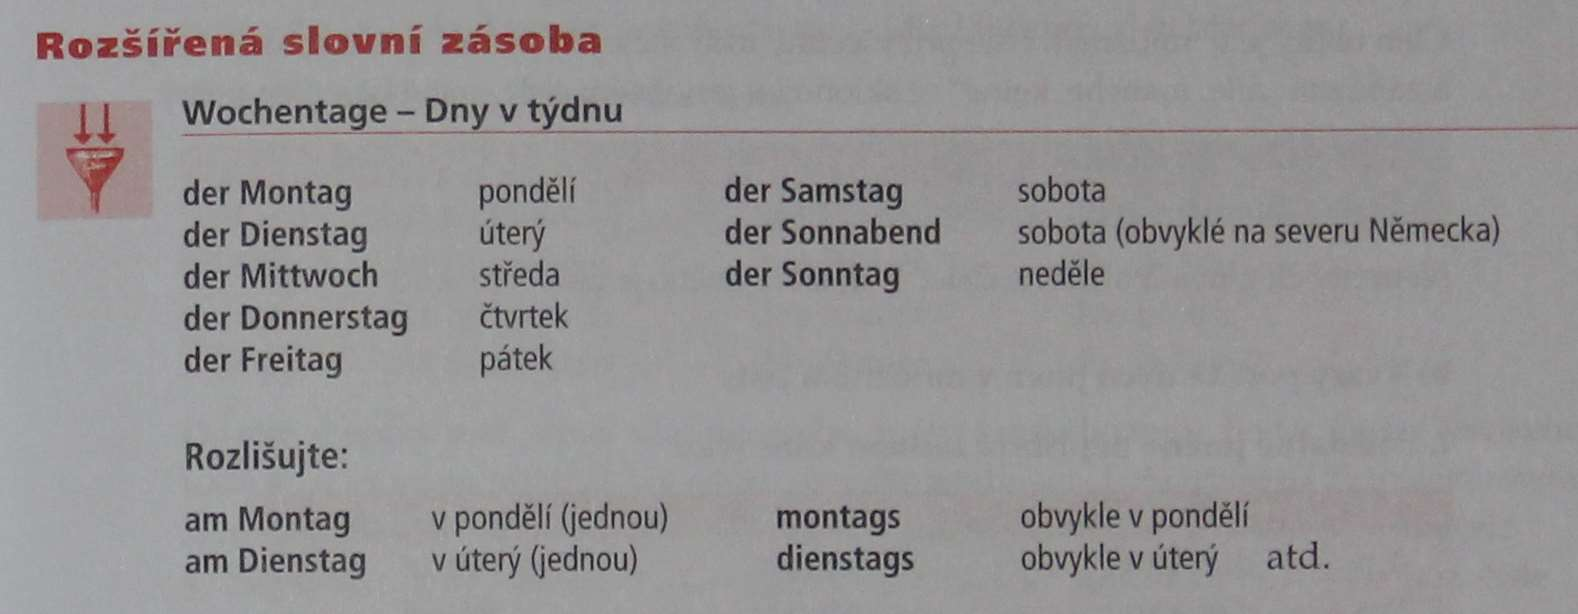
\includegraphics[width=1\linewidth]{L4_Wortschatz03.jpg}
      \caption*{ }
      \label{NJ:fig_L4_Wortschatz03}
    \end{figure}
    
    \subsection*{Skloňování podstatných jmen v množném čísle}
      \begin{itemize} % L4_Grammatik01.jpg
        \item \textbf{Skloňování určitého členu a některých zájmen v množném čísle:}
              \begin{table}[ht!]   % L4_Redensart01.jpg
                \hspace*{5em}
                \begin{tabular}{l|ll}
                  \hline
                  l.p. & die & meine, keine, alle, manche     \\
                  2.p. & der & meiner, keiner, aller, mancher \\
                  3.p. & den & meinen, keinen, allen, manchen \\
                  4.p. & die & meine, keine, alle, manche     \\
                  \hline
                \end{tabular}
                \caption*{ }
              \end{table}
              
              Člen určitý je v množném čísle pro všechny rody stejný. Všechna přivlastňovací 
              zájmena a zájmena „alle, manche, keine" se skloňují v množném čísle stejně jako člen 
              určitý.
              \begin{itemize}
                \addtolength{\itemindent}{5em}
                \item Haben Sie ein Kind?
                \item Haben Sie Kinder?
              \end{itemize}
              Neurčitý člen nemá množné číslo, podstatné jméno je pak bez členu.
        \item \textbf{Tvary podstatných jmen v množném čísle:}
          \begin{itemize}
            \item \textbf{Podstatné jméno nepřibírá žádnou koncovku}
              \begin{table}[ht!]   % L4_Grammatik02.jpg
                \hspace*{4em}
                \begin{tabular}{l|lll}
                       & \textbf{der Vater}  & \textbf{die Mutter}  & \textbf{das Rätsel}  \\
                  \hline
                  1.p. & die Vater           & die Mütter           & die Rätsel           \\
                  2.p. & der Väter           & der Mütter           & der Rätsel           \\
                  3.p. & den Vätern          & den Müttern          & den Rätseln          \\
                  4.p. & die Väter           & die Mütter           & die Rätsel           \\
                  \hline
                \end{tabular}
                \caption*{ }
              \end{table}
        
              Bez koncovky jsou především podstatná jména mužského a středního rodu, která končí v 
              jednotném čísle na \textbf{-er}, \textbf{-el}, \textbf{-en} a zdrobněliny, které jsou 
              vždy středního rodu a tvoří se příponami \textbf{-chen} a \textbf{-lein}. Z 
              podstatných jmen ženského rodu jsou bez koncovky jen dvě - \emph{„die Mutter"} a 
              \emph{„die Tochter"}. Některá podstatná jména této skupiny přehlasují (tzn. mění 
              kmenovou samohlásku: \emph{a - ä}, \emph{u - ü}, \emph{o - ö}, \emph{au - äu}).
      
            \item \textbf{Podstatné jméno přibírá v množné čísle koncovku -e}
              \begin{table}[ht!]   % L4_Grammatik02.jpg
                \hspace*{4em}
                \begin{tabular}{l|lll}
                       & \textbf{der Freund}   & \textbf{die Stadt}   & \textbf{das Jahr}    \\
                  \hline
                  1.p. & die Freunde           & die Städte           & die Jahre            \\
                  2.p. & der Freunde           & der Städte           & der Jahre            \\
                  3.p. & den Freunde\textbf{n} & den Städte\textbf{n} & den Jahre\textbf{n}  \\
                  4.p. & die Freunde           & die Städte           & die Jahre            \\
                  \hline
                \end{tabular}
                \caption*{ }
              \end{table}

              Tato skupina je zastoupena především u mužského rodu. V ženském rodě je zastoupena 
              pouze asi 40 podstatnými jmény, která přehlasují vždy, je-li v kmeni přehlasovatelná 
              samohláska. Podst. jména mužského a středního rodu přehlasují jen někdy.
              
            \item \textbf{Množné číslo má koncovku -er}
            \item \textbf{Množné číslo má koncovku -(e)n}
            \item \textbf{Množné číslo přebírá koncovku -s (pouze u některých cizích slov)}\newline
         \end{itemize}
      \end{itemize}
    
    \begin{figure}[ht!]
      \centering
      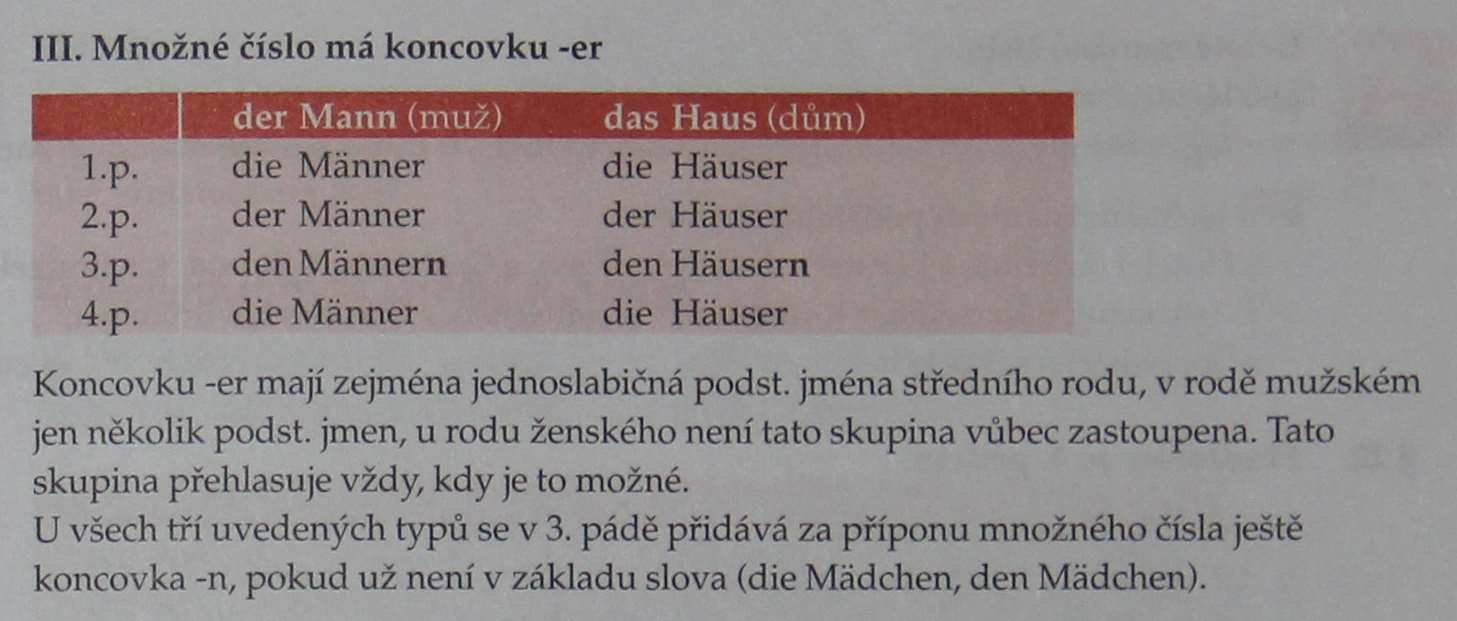
\includegraphics[width=1\linewidth]{L4_Grammatik03.jpg}
      \caption*{ }
      \label{NJ:fig_L4_Grammatik03}
    \end{figure}
    
    \begin{figure}[ht!]
      \centering
      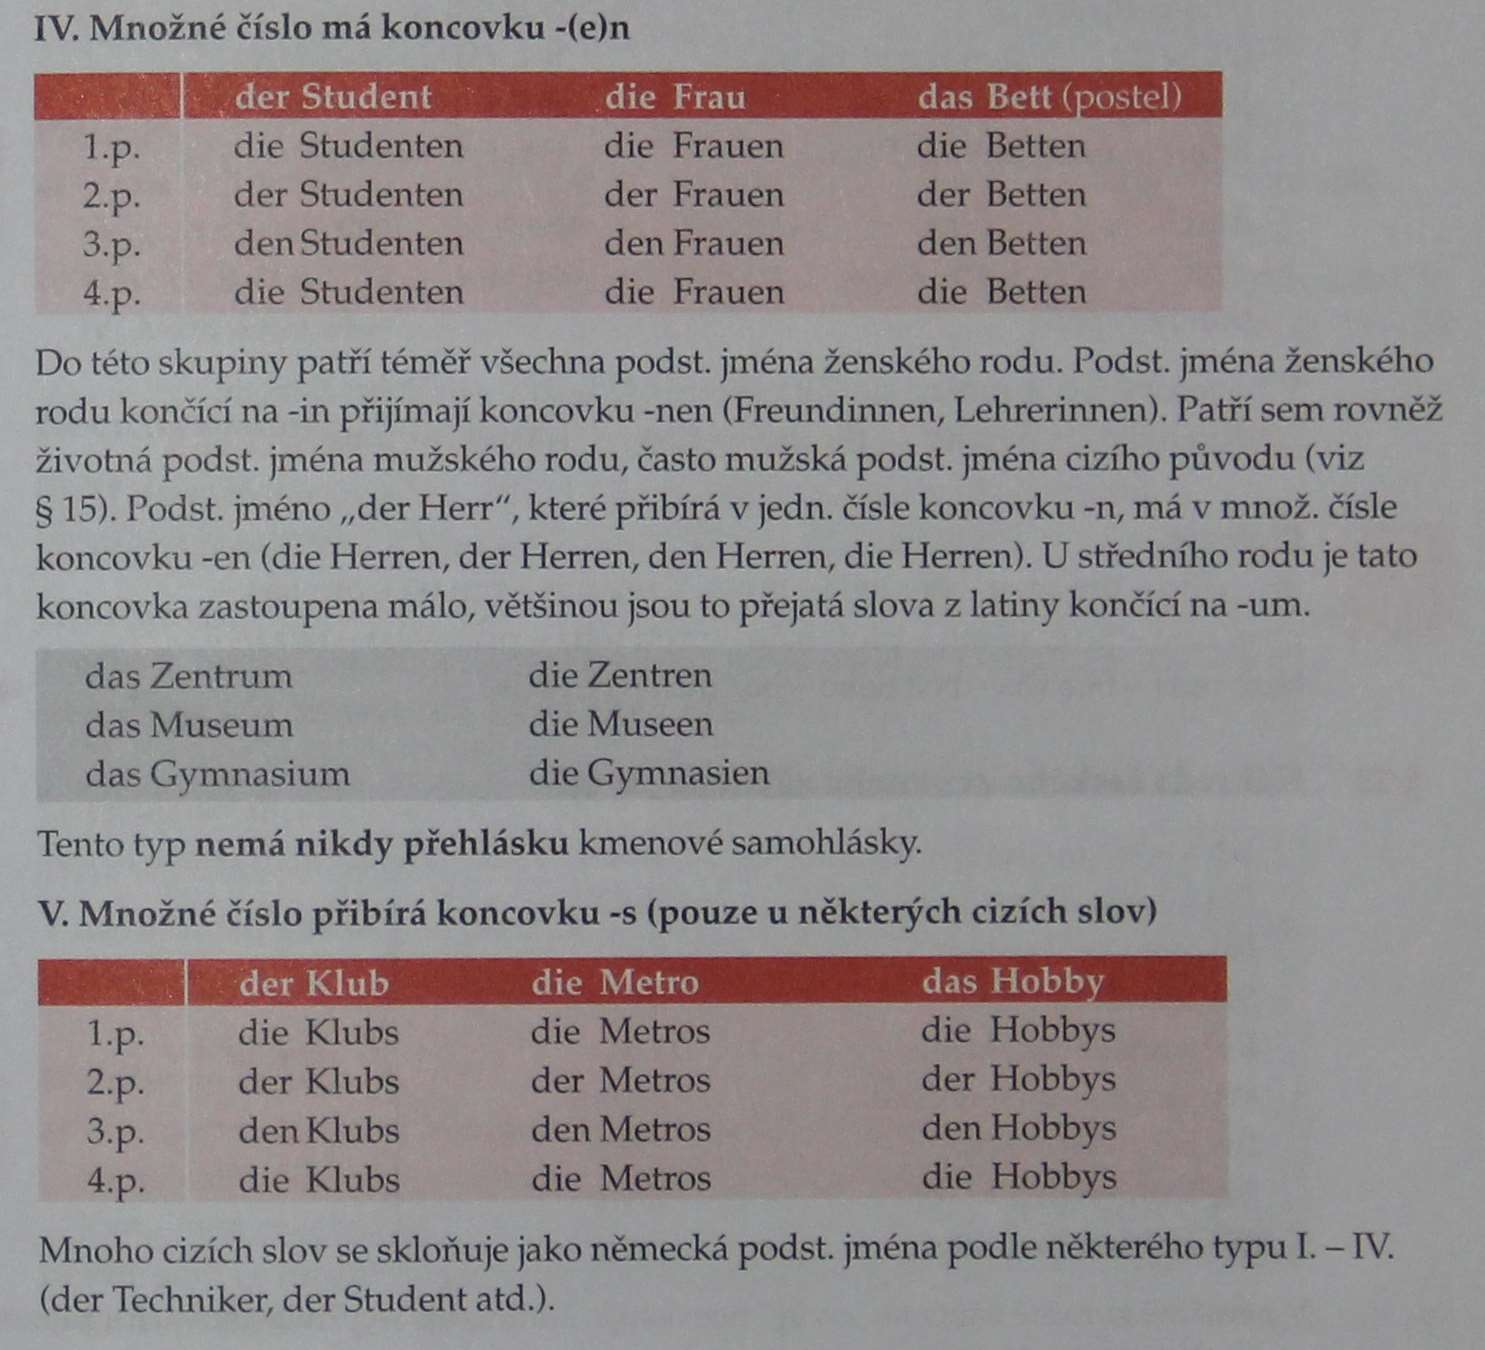
\includegraphics[width=1\linewidth]{L4_Grammatik04.jpg}
      \caption*{ }
      \label{NJ:fig_L4_Grammatik04}
    \end{figure}
    
    \begin{figure}[ht!]
      \centering
      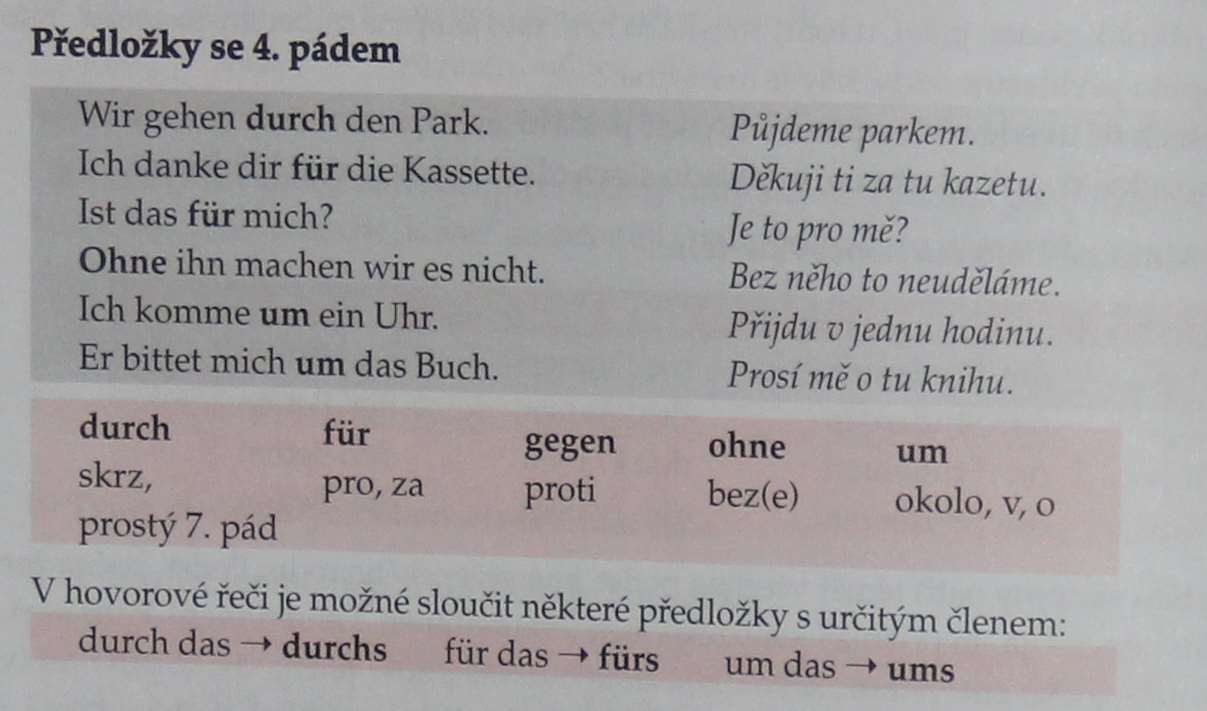
\includegraphics[width=1\linewidth]{L4_Grammatik05.jpg}
      \caption*{ }
      \label{NJ:fig_L4_Grammatik05}
    \end{figure}
    
    \begin{figure}[ht!]
      \centering
      
\includegraphics[width=1\linewidth]{L4_Grammatik06.jpg}
      \caption*{ }
      \label{NJ:fig_L4_Grammatik06}
    \end{figure}
    
    \begin{figure}[ht!]
      \centering
      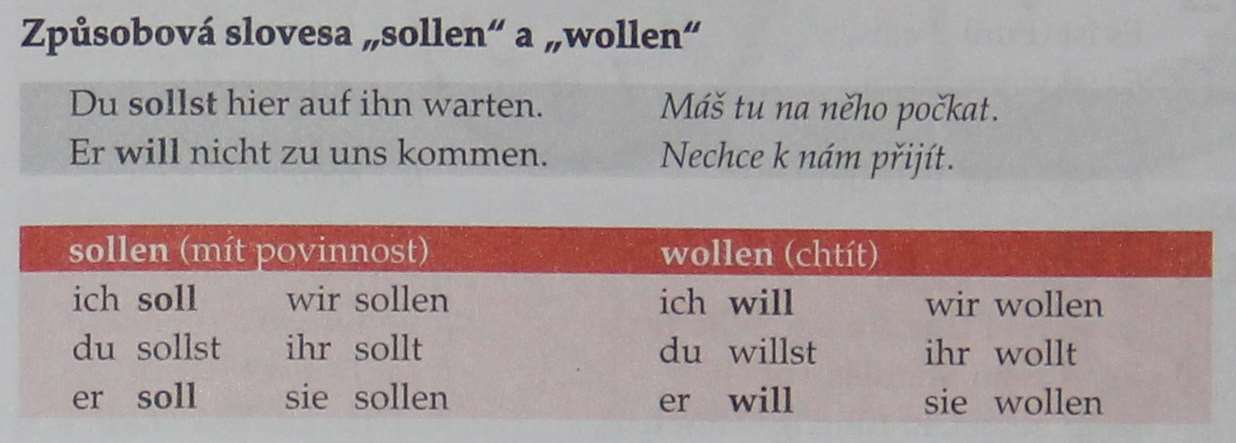
\includegraphics[width=1\linewidth]{L4_Grammatik07.jpg}
      \caption*{ }
      \label{NJ:fig_L4_Grammatik07}
    \end{figure}
    
    \begin{figure}[ht!]
      \centering
      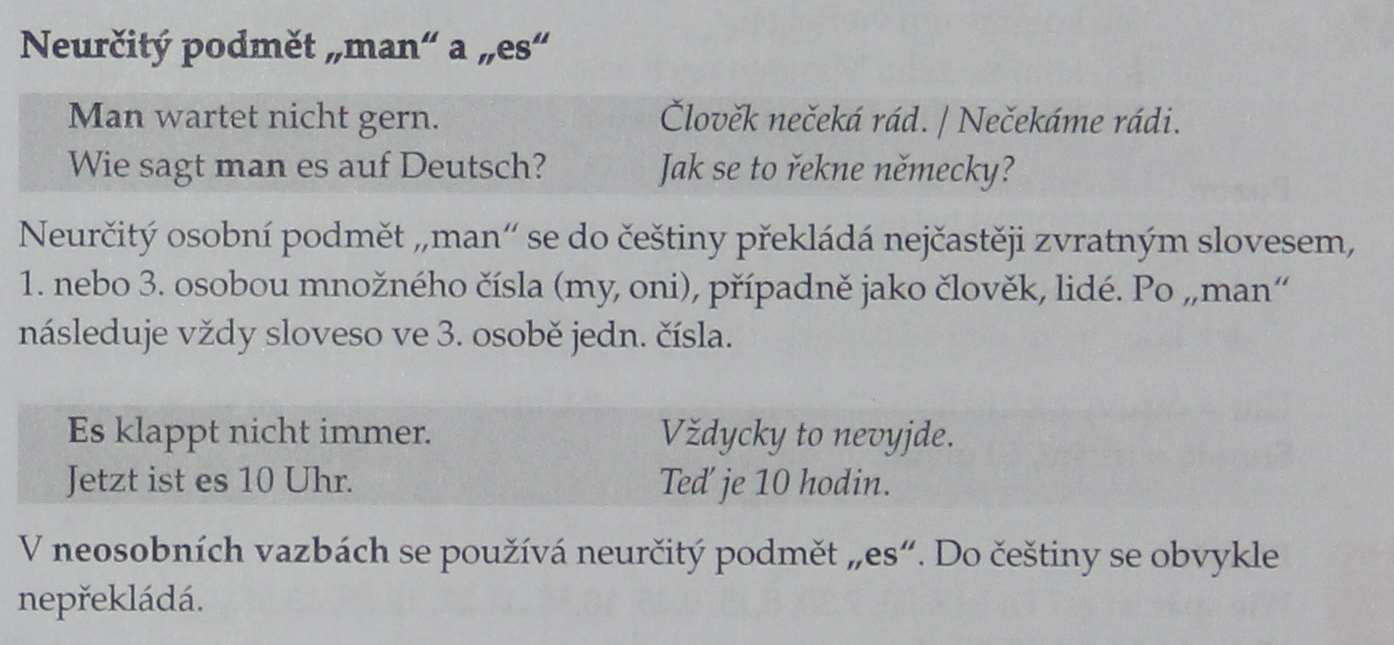
\includegraphics[width=1\linewidth]{L4_Grammatik08.jpg}
      \caption*{ }
      \label{NJ:fig_L4_Grammatik08}
    \end{figure}
  % !TeX spellcheck = de_DE
%================ Kapitola 5: Guten Appetit! =======================================================
\setchaptertoc
\chapter{Lektion 5: Guten Appetit!}\label{NJ:chap_N1_L5}
  
  \section*{Slovní zásoba}

      



















































  % !TeX spellcheck = de_DE
%================ Kapitola 6: Karin und Horst ziehen um ============================================
\chapter{Lektion 6: Karin und Horst ziehen um}\label{NJ:chap_N1_L6}
\minitoc
  
  \section{Slovní zásoba}
    \begin{table}[ht!]   % L4_Wortschatz01.jpg
      \centering
      \begin{tabular}{llll}
        \hline
          der, die, das erste     & první    & r, e, s nächste        & příští, další, nejbližší  \\
          eigen                   & vlastní  & e Prüfung, -, en (in)  &  zkouška (z)              \\
          aussehen, du siehst aus & vypadat  &  ablegen, du legst ab  & složit (zkoušku)          \\
          r Flur, (e)s, e         & předsíň  & e Geduld, -, 0         & trpělivost                \\
          e Tür, -, en            & dveře    & weil                   & protože                   \\
          führen                  & vést     & jeder, jede, jedes     & každý, každá, každé       \\
          schlafen, du schläfst   & spát     &  lieber                & raději                    \\
          s Schlafzimmer, s, -    & ložnice  & eng                    & úzký, úzce, těsný, -ě     \\
          e Küche, -, n           & kuchyně  & e Anbaumöbel (mn.č.)   & sektorový (stavebnicový)  \\
          s Bad, (e)s, ä-er       & koupelna &                        &  nábytek                  \\
          eingerichtet            & zařízený &  r Stuhl, (e)s, ü-e    & židle                     \\
          s Bett, es, en          & postel   & sitzen                 &  sedět                    \\
          s Kleid, (e)s, er       & šaty (dámské) & nachdenken, du    & přemýšlet (o)             \\
          r Schrank, (e)s, ä-e    & skříň         & denkst nach       &                           \\
          hell                    & světlý, -e    &  (über 4.p.)      &                           \\
          e Möbel (mn.c.)         & nábytek       & s Studenten(wohn)-& kolej                     \\
          an (3./4.p.)            & na (svislé ploše), u, k   & heim, (e)s, e  &                  \\
          recht                   & pravý         & lieb              & milý, -e                  \\
          e Wand, -, ä-e          & stěna         & vielmals          & mnohokrát                 \\
          stehen                  & stát          &  r Brief, (e)s, e & dopis                     \\
          r Fernseher, s, -       & televizor     & wissen, ich weiß  & vědět                     \\
          bequem                  & pohodlný, -ě  & billig            & levný, -ě, laciný, -ě     \\
          neben (3./4.p.)         & vedle         & bezahlen          & (za)platit                \\
          e Sitzgarnitur, -, en   & sedací souprava  & e Miete, -, n  & nájemné                   \\
          zwischen (3./4.p.)      & mezi (dvěma)  & pro               &  za, pro, na              \\
          s Sofa, s, s            & pohovka       & r Stock, (e)s, Stock-  & poschodí             \\
          r Sessel, s, -          & křeslo        & werke             &                           \\
          r Couchtisch,(e)s.      & konferenční stolek  & modern      & moderní                   \\
          e [kauč-]               &               & zusammen          & společně, dohromady       \\
          unter (3./4.p.)         & pod, mezi (více) & s Studienjahr, (e)s, e  & ročník (studia)  \\
          s Fenster, s, -         & okno          & e Fachrichtung, -, en      & obor, zaměření   \\
          e Blume, -, n           & květina       & helfen, du hilfst & pomáhat, pomoci           \\
          e Ecke, -, n            & roh, kout     & r Briefumschlag,  & obálka                    \\
          verschieden             & různý, -ě     & (e)s, ä-e         &                           \\
          s Heft, (e)s, e         & sešit         &  ergänzen         & doplnit, -ňovat           \\
          e Zeitung, -, en        & noviny        & geboren           & narozen(ý)                \\
          e Zeitschrift, -, en    & časopis       &                   &              \\
         \hline
      \end{tabular}
      \caption*{}
    \end{table}
      



















































} % DEBUG was off
}
% ============== Appendix ========================
\backmatter 
% ============== Bibliography ====================
  \printbibliography[title={Bibliografie}]
  \addcontentsline{toc}{chapter}{Seznam literatury}
\end{document}